\documentclass[11pt,a4paper,oneside,english]{book} 

\usepackage[a4paper]{geometry}
\geometry{verbose, tmargin=4cm, bmargin=4cm, lmargin=3cm, rmargin=3cm, headsep=0.5cm, footskip=1cm}
\usepackage[latin1]{inputenc}

\usepackage{siunitx} 
\usepackage{tikz}
\usepackage{blox}
\usepackage{pgfplots}
\pgfplotsset{compat=1.14}
\usepackage{subfigure}
\usepackage{xcolor,colortbl}
\usepackage{array}
\newcolumntype{P}[1]{>{\centering\arraybackslash}p{#1}}
\newcolumntype{M}[1]{>{\centering\arraybackslash}m{#1}}
\newcolumntype{L}[1]{>{\arraybackslash}m{#1}}
\usetikzlibrary{positioning, automata, arrows, quotes, angles, calc, trees, chains,	
decorations.pathreplacing, decorations.pathmorphing, shapes, matrix}

%For drawing folders
\usepackage{forest}
\definecolor{forange}{RGB}{233,84,32}
\newcommand\myfolder[2][forange]{%
	\begin{tikzpicture}[overlay]
	\begin{scope}[xshift=20pt]
	\filldraw[rounded corners=1pt,fill=#1,draw=white,double=black]
	(-23pt,10pt) -- ++(3pt,5pt) -- ++(18pt,0pt) -- ++(40:3pt) -- ++(9pt,0pt) -- ++(-40:3pt)
	-- (20pt,15pt) -- (23pt,10pt) -- cycle;
	\filldraw[rounded corners,draw=white,double=black,top color=#1,bottom color=#1!30]
	(-22pt,-12pt) -- ++(44pt,0pt) -- (25pt,12pt) coordinate (topr) -- ++(-50pt,0pt) coordinate 
	(topl) -- cycle;
	\end{scope}  
	\end{tikzpicture}%
	\makebox[35pt]{\raisebox{-3pt}{{\ttfamily/#2}}}%
}

%Random variables generator
\usepackage{pgfplots}
\pgfplotsset{compat=newest}
\def\xlist{4}
\def\ylist{4}

\newcommand{\fillrandomly}[4]{
	\pgfmathsetmacro\diameter{#3*2}
	%\draw (0,0) rectangle (#1,#2);
	\foreach \i in {1,...,#4}{
		\pgfmathsetmacro\x{rnd*#1}
		\pgfmathsetmacro\y{rnd*#2}
		\xdef\collision{0}
		\foreach \element [count=\i] in \xlist{
			\pgfmathtruncatemacro\j{\i-1}
			\pgfmathsetmacro\checkdistance{ sqrt( ({\xlist}[\j]-(\x))^2 + ({\ylist}[\j]-(\y))^2 ) }
			\ifdim\checkdistance pt<\diameter pt
			\xdef\collision{1}
			\breakforeach
			\fi
		}
		\ifnum\collision=0
		\xdef\xlist{\xlist,\x}
		\xdef\ylist{\ylist,\y}
		\draw [fill=black, thick] (\x,\y) circle [radius=#3];
		\fi 
		
	}
}

\usepackage{fancyhdr}
\pagestyle{fancy}
\renewcommand{\chaptermark}[1]{\markboth{#1}{}}
\renewcommand{\sectionmark}[1]{\markright{\thesection\ #1}}
\fancyhf{}
\fancyhead[LE,RO]{\bfseries\thepage}
\fancyhead[LO]{\bfseries\rightmark}
\fancyhead[RE]{\bfseries\leftmark}
\renewcommand{\headrulewidth}{0.5pt}
\renewcommand{\footrulewidth}{0.5pt}
\setlength{\headheight}{14.5pt}

\usepackage{amsmath, amsfonts, amssymb, amsthm}
\usepackage{mathtools}
\usepackage{latexsym}
\usepackage{lmodern}
\usepackage[T1]{fontenc}
\newcommand*\rfrac[2]{{}^{#1}\!/_{#2}}

\usepackage{setspace}

\usepackage{hyperref}  
\hypersetup{
	pdftitle={Drawing examples in LaTeX},
	pdfauthor={Giuseppe Silano},
	pdfsubject={The aim of this file is to help people interested in learning how to use LaTeX for 
	drawing. In particular, already structured examples can help through the provided source code 
	on how to use the code for its own purposes.},
	pdfkeywords={LaTeX, open-source, source code, tikzpicture, repository}}           

\begin{document}

\frontmatter

\renewcommand{\theequation}{\arabic{equation}}
\renewcommand{\thesection}{\arabic{section}}  
\renewcommand{\theequation}{\arabic{chapter}.\arabic{equation}}
\renewcommand{\thesection}{\arabic{chapter}.\arabic{section}}
\setcounter{chapter}{1}

\title{
	\textbf{\huge{Drawing examples in \LaTeX}}
	\\
	\vspace{1cm}
}
	
\author{\textsc{Giuseppe Silano}
\date{\today}
} 

\maketitle

\mainmatter

\pagenumbering{roman}

\tableofcontents

\setcounter{page}{0}
\setcounter{chapter}{0}

\onehalfspacing

\chapter*{Introduction}
\addcontentsline{toc}{chapter}{Introduction}

\section*{The aim of document}
\label{sec:aimOfTheDocument}
\addcontentsline{toc}{section}{The aim of document}

The aim of this file is to help people interested in learning how to use \LaTeX~for drawing. In 
particular, already structured examples will help to develop one's own through the source code 
provided. The draws have been made during my research activity as PhD candidate.

The file is divided into four main chapters (parts):

\begin{itemize}
	
	\item \textit{Block Diagrams} (see Ch.~\ref{chapter:blockDiagram}): this part contains block 
	diagrams;
	
	\item \textit{Matlab Plots} (see Ch.~\ref{chapter:matlabPlots}): this part contains 
	MATLAB\textsuperscript{\textregistered} and the 
	MATLAB package \textit{matlab2tikz}\footnote{It is available at the 
	link~\url{https://github.com/matlab2tikz/matlab2tikz}}.
	
	\item \textit{Drawing on Images} (see Ch.~\ref{chapter:drawingOnImages}): this part contains 
	draws made on image files;
	
	\item \textit{Various} (see Ch.~\ref{chapter:various}): this part contains several drawings 
	that do not belong to the sections 
	listed above.
	
\end{itemize}


\mainmatter

\pagenumbering{arabic}

\onehalfspacing

\chapter{Block Diagram}
\label{chapter:blockDiagram}

\newcounter{blockDiagram}
\setcounter{blockDiagram}{0}
\stepcounter{blockDiagram}

\section{Example \theblockDiagram}
\stepcounter{blockDiagram}


\begin{figure}[h]
	\centering
	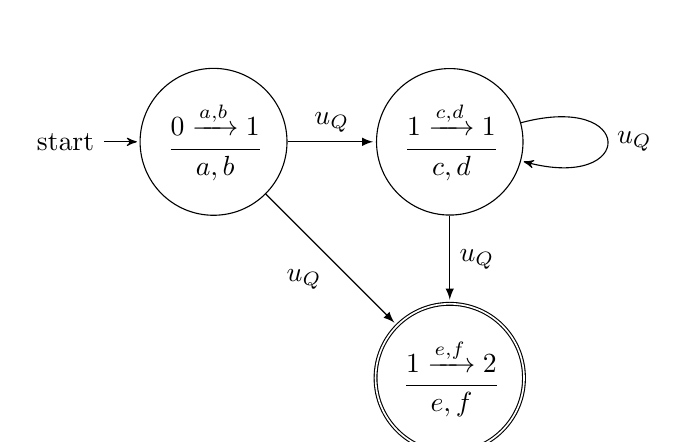
\begin{tikzpicture}[>=stealth',shorten >=1pt,node distance=2cm,on grid,auto] 
	
	%Automata states
	\node[state,initial] (q_0)   {$\cfrac{0 \xrightarrow[]{a,b} 1}{a,b}$}; 
	\node[state] (q_1) [right=3cm of q_0] {$\cfrac{1 \xrightarrow[]{c,d} 1}{c,d}$}; 
	\node[state,accepting] (q_2) [below=3cm of q_1] {$\cfrac{1 \xrightarrow[]{e,f} 2}{e,f}$}; 
	
	%Automata Paths
	\path[-latex] 
	(q_0) edge 				node 	    {$u_Q$} (q_1)
	edge				node [swap] {$u_Q$} (q_2)
	(q_1) edge 				node 		{$u_Q$} (q_2)
	edge [loop right] node 		{$u_Q$} ();
	
	\end{tikzpicture}

\end{figure}

\section{Example \theblockDiagram}
\stepcounter{blockDiagram}

\begin{figure}[h]
	\begin{center}
		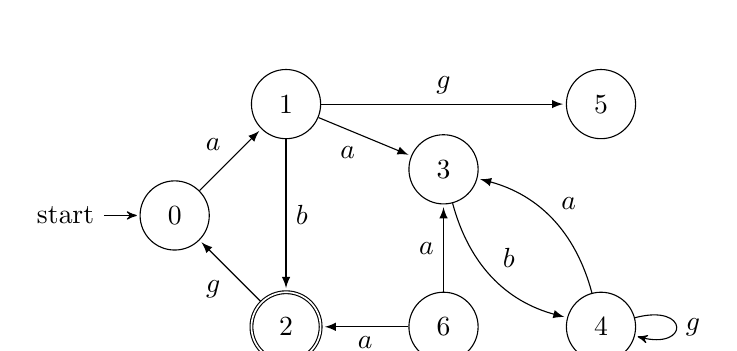
\begin{tikzpicture}[>=stealth',shorten >=1pt,node distance=2cm,on grid,auto] 
		
		%Automata states
		\node[state,initial] (q_0)   {$0$}; 
		\node[state] (q_1) [above right=of q_0] {$1$}; 
		\node[state,accepting] (q_2) [below right=of q_0] {$2$}; 
		\node[state] (q_6) [right=of q_2] {$6$};
		\node[state] (q_3) [above =of q_6] {$3$};
		\node[state] (q_4) [right=of q_6] {$4$};
		\node[state] (q_5) [right=4cm of q_1] {$5$};
		
		%Automata paths
		\path[-latex] 
		(q_0) edge 				node 		{$a$} (q_1)
		(q_1) edge 				node 		{$g$} (q_5)
		edge 				node [swap]	{$a$} (q_3)
		edge 				node 		{$b$} (q_2)
		(q_3) edge [bend right]	node 		{$b$} (q_4)
		(q_4) edge [loop right] node 		{$g$} ()
		edge [bend right] node [swap]	{$a$} (q_3)
		(q_6) edge				node 		{$a$} (q_3)
		edge 				node 		{$a$} (q_2)
		(q_2) edge 				node 		{$g$} (q_0);
		
		\end{tikzpicture}
	\end{center}

\end{figure}

\section{Example \theblockDiagram}
\stepcounter{blockDiagram}

\begin{figure}[h]
	\begin{center}
		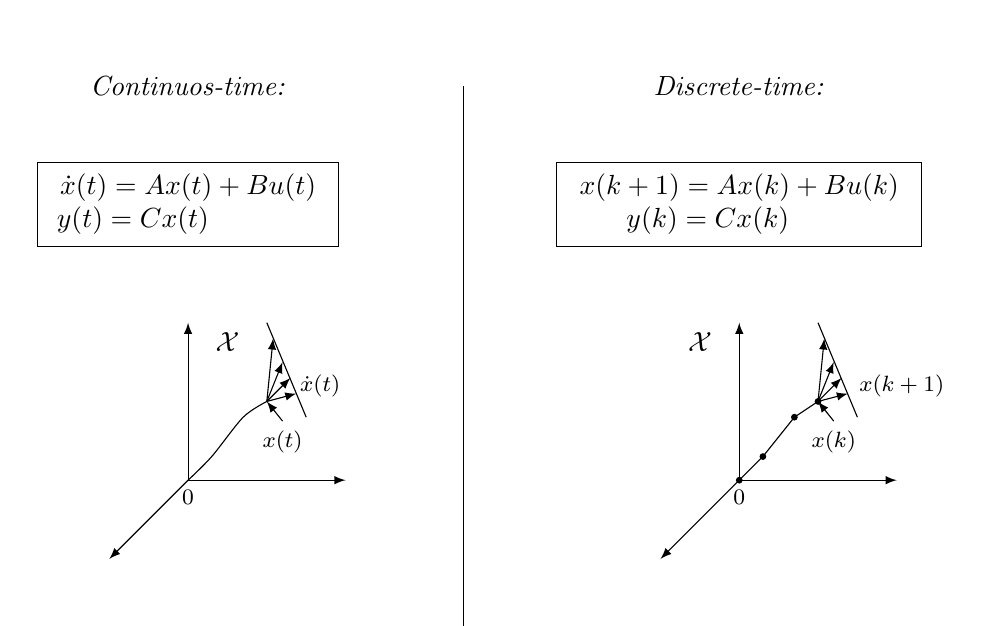
\begin{tikzpicture}
		
		%Lines separiting the two plots
		\draw[-] (0,0) coordinate -- (0,-7.0) coordinate;
		
		%Continuous-time equations
		\node (continuosTime) at (-3.5,0) [text centered]{\textit{Continuos-time:}};
		
		\node (rettangoloContinuo) at (-3.5,-1.5) []{
			
			\boxed{
				\begin{array}{cc}
				\dot{x}(t)=Ax(t)+Bu(t)\\
				\hspace{-1.4cm}y(t)=Cx(t)
				\end{array}
			}
		};
		
		%The reference system
		\draw[-latex] (-3.5,-5.0) coordinate node[below]{\footnotesize{$0$}} -- (-3.5,-3.0) 
		coordinate;
		\draw[-latex] (-3.5,-5.0) coordinate -- (-1.5,-5.0) coordinate;
		\draw[-latex] (-3.5,-5.0) coordinate -- (-4.5,-6.0) coordinate;
		
		%Smooth curve
		\draw [black] plot [smooth] coordinates {(-3.5,-5.0) (-3.2,-4.7) (-2.8,-4.2) (-2.5,-4.0)};
		
		%Line
		\draw (-2.0,-4.2) coordinate -- (-2.5,-3.0) coordinate;
		
		%Arrows
		\draw[-latex] (-2.5,-4.0) coordinate -- (-2.125,-3.9) coordinate;
		\draw[-latex] (-2.5,-4.0) coordinate -- (-2.2,-3.7) coordinate;
		\draw[-latex] (-2.5,-4.0) coordinate -- (-2.3,-3.5) coordinate;
		\draw[-latex] (-2.5,-4.0) coordinate -- (-2.42,-3.2) coordinate;
		
		%Arrows with x
		\draw[-latex] (-2.3,-4.25) coordinate node[below]{\footnotesize{$x(t)$}} -- (-2.5,-4.0) 
		coordinate;
		
		%Callygraphic X
		\draw (-3.0,-3.0) coordinate node[below]{$\mathcal{X}$};
		
		%Xdot depicting
		\draw (-2.2,-3.8) node[right]{\footnotesize{$\dot{x}(t)$}};
		
		
		%%%%%%%%%%%%%%%%%%%%%%%%%%%%%%%%%%%%%
		%Discre-time equations
		\node (discreteTime) at (3.5,0) [text centered]{\textit{Discrete-time:}};
		
		\node (rettangoloContinuo) at (3.5,-1.5) []{
			
			\boxed{
				\begin{array}{cc}
				x(k+1)=Ax(k)+Bu(k)\\
				\hspace{-0.8cm}y(k)=Cx(k)
				\end{array}
			}
		};
		
		%Reference systems
		\draw[-latex] (3.5,-5.0) coordinate node[below]{\footnotesize{$0$}} -- (3.5,-3.0) 
		coordinate;
		\draw[-latex] (3.5,-5.0) coordinate -- (5.5,-5.0) coordinate;
		\draw[-latex] (3.5,-5.0) coordinate -- (2.5,-6.0) coordinate;
		
		%Smooht curve
		\draw[black] plot coordinates {(3.5,-5.0) (3.8,-4.7) (4.2,-4.2) (4.5,-4.0)};
		\filldraw (3.5,-5.0) circle (1pt);
		\filldraw (3.8,-4.7) circle (1pt);
		\filldraw (4.2,-4.2) circle (1pt);
		\filldraw (4.5,-4.0) circle (1pt);
		
		%Line
		\draw (5.0,-4.2) coordinate -- (4.5,-3.0) coordinate;
		
		%Callygraphics x
		\draw (3.0,-3.0) coordinate node[below]{$\mathcal{X}$};
		
		%Depecting xk+a
		\draw (4.9,-3.8) node[right]{\footnotesize{$x(k+1)$}};
		
		%Arrow with x
		\draw[-latex] (4.7,-4.25) coordinate node[below]{\footnotesize{$x(k)$}} -- (4.5,-4.0) 
		coordinate;
		
		%Arrows representation
		\draw[-latex] (4.5,-4.0) coordinate -- (4.88,-3.9) coordinate;
		\draw[-latex] (4.5,-4.0) coordinate -- (4.8,-3.7) coordinate;
		\draw[-latex] (4.5,-4.0) coordinate -- (4.7,-3.5) coordinate;
		\draw[-latex] (4.5,-4.0) coordinate -- (4.58,-3.2) coordinate;
		
		\end{tikzpicture}
	\end{center}
\end{figure}


\section{Example \theblockDiagram}
\stepcounter{blockDiagram}

\begin{figure}[h]
	\begin{center}
			\begin{tikzpicture}[node distance=2cm]
			
			%Blocks
			\node (virtualReality) at (2.5,0) [rectangle, draw, text centered, minimum width=2.5cm, 
			minimum height=1cm] {Virtual Reality};
			\node (classifier) at (-2,0) [rectangle, draw, text centered, minimum width=2.5cm, 
			minimum height=1cm] {Classifier};
			\node (computing) at (-3,3)  [rectangle, draw, text centered, minimum width=2.5cm, 
			minimum height=1cm] {Computing};
			\node (controller) at (0.5,3) [rectangle, draw, text centered, minimum 
			width=2.5cm,minimum height=1cm] {Controller};
			\node (car) at (7.8,-0.25) [rectangle, draw, text centered, minimum width=2.5cm, 
			minimum height=1cm] {Car};
			\node (drone) at (4.0,3) [rectangle, draw, text centered, minimum width=2.5cm, minimum 
			height=1cm] {Drone};
			
			%Links
			\draw [-latex] (virtualReality.west) -- (classifier.east);
			\draw [-latex] (classifier.west) -- (-5.0,0) -- (-5.0,3) -- (computing.west);
			\draw [-latex] (computing.east) -- (controller.west);
			\draw [-latex] (controller.east) -- (drone.west);
			\draw [-latex] (car.west) -- (3.9,-0.25);
			\draw [-latex] (drone.east) -- (6.0,3) -- (6.0,0.255) -- (3.9,0.255);
			\draw [-latex] (5.7,3) -- (5.7,4.5) -- (0.5,4.5) -- (controller.north);
			\node (circle) at (5.7,3) [circle, draw, scale=0.4, fill=black] {};
			
			\end{tikzpicture}
	\end{center}

\end{figure}

\newpage

\section{Example \theblockDiagram}
\stepcounter{blockDiagram}

\begin{figure}[h]
	\begin{center}
		\begin{tikzpicture}
		
		%Reference system
		\draw[dashed] (0,0) coordinate -- (0,1) coordinate;
		\draw[-latex] (0,1) coordinate -- (0,3) coordinate node[above left]{$y$};
		\draw[dashed] (0,0) coordinate -- (1,0) coordinate;
		\draw[-] (1,0) coordinate -- (3,0) coordinate node[above right]{$-x$};
		\draw[dashed] (0,0) coordinate -- (-1.2,0) coordinate;
		\draw[-latex] (-1.2,0) coordinate -- (-3,0) coordinate node[above left]{$x$};
		\node (circle) at (0,0) [circle, draw, dashed, minimum size=0.5cm]{};
		\node[circle,draw,black,scale=0.3, fill=black] at (0,0) {};
		\draw (0,-0.25) coordinate node[below left]{$z$};
		
		%Camera
		\draw[-, line width=1.25pt] (1,1) coordinate -- (-1,1) coordinate;
		\draw[-, line width=1.25pt] (1,-1) coordinate -- (-1,-1) coordinate;
		\draw[-, line width=1.25pt] (1,-1) coordinate -- (1,1) coordinate;
		\draw[-, line width=1.25pt] (-1,-1) coordinate -- (-1,1) coordinate;
		
		\draw[-, line width=1.25pt] (-1,-1) coordinate -- (-1.2,-1.2) coordinate;
		\draw[-, line width=1.25pt] (-1,1) coordinate -- (-1.2,1.2) coordinate;
		\draw[-, line width=1.25pt] (-1.2,1.2) coordinate -- (-1.2,-1.2) coordinate;
		
		\end{tikzpicture}
	\end{center}
	
\end{figure}


\section{Example \theblockDiagram}
\stepcounter{blockDiagram}

\begin{figure}[h]
	\begin{center}
		\scalebox{0.8}{
			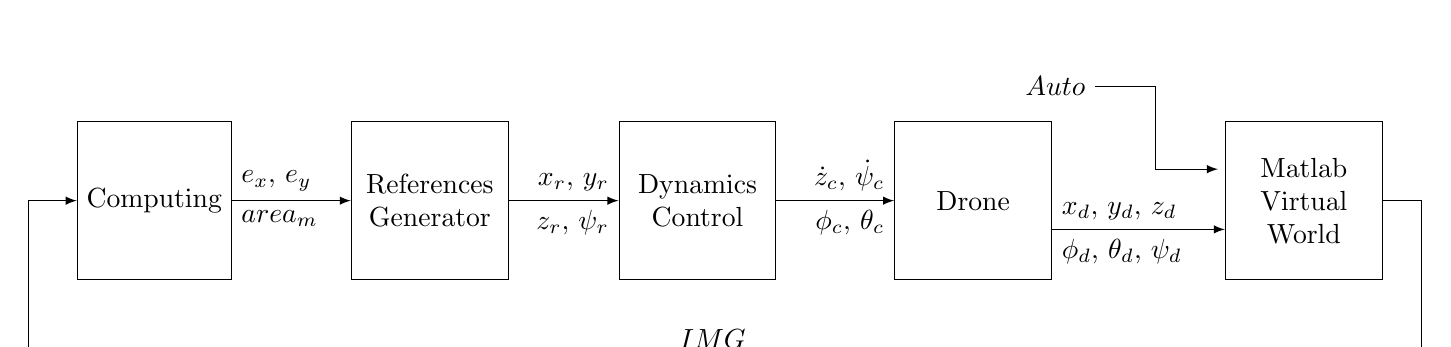
\begin{tikzpicture}
			
			%Computing block
			\node (computing) at (-4.2,0) [draw, rectangle, text centered, minimum width=1cm, 
			minimum height=2cm]{Computing};
			
			%Reference generator
			\node (referenceGenerator) at (-0.7,0) [draw, rectangle, minimum width=1cm, text 
			width=5em, minimum height=2cm, text centered]{References\\ Generator};
			
			%Trajectory controller
			\node (trajectoryController) at (2.7,0) [draw, rectangle, minimum width=1cm, minimum 
			height=2cm, text centered, text width=5em]{Dynamics\\ Control};
			
			%Drone
			\node (drone) at (6.2,0) [draw, rectangle, minimum width=1cm, minimum height=2cm, text 
			centered, text width=5em]{Drone};
			
			%Matlab virtual world
			\node (virtualWorld) at (10.4,0) [draw, rectangle, minimum width=1cm, minimum 
			height=2cm, text centered, text width=5em]{Matlab \\Virtual World};
			
			%Links among blocks
			\draw[-latex] (computing.east) node[above right]{$e_x,\,e_y$} node[below 
			right]{$area_m$}-- (referenceGenerator.west);
			\draw[-latex] (referenceGenerator.east) -- (trajectoryController.west) node[below 
			left]{$z_r,\,\psi_r$} node[above left]{$x_r,\,y_r$};
			\draw[-latex] (trajectoryController.east) -- (drone.west) node[above 
			left]{$\dot{z}_c,\,\dot{\psi}_c$} node[below left]{$\phi_c,\,\theta_c$};
			\draw[-latex] (drone.-20) node[below right]{$\phi_d,\,\theta_d,\,\psi_d$} node[above 
			right]{$x_d,\,y_d,\,z_d$} -- (virtualWorld.200);
			\draw[-latex] (virtualWorld.east) -- (11.9,0) coordinate -- (11.9,-2.0) coordinate 
			--(-5.8,-2.0) coordinate -- (-5.8,0) coordinate -- (computing.west);
			\draw (2.35,-2.0) coordinate node[above right]{$IMG$};
			
			%Link for connecting the car block
			\draw[-latex] (7.75,1.45) coordinate node[left]{$Auto$}-- (8.52,1.45) coordinate -- 
			(8.52,0.4) coordinate -- (9.31,0.4) coordinate;
			
			\end{tikzpicture}
		}
	\end{center}
	
\end{figure}


\section{Example \theblockDiagram}
\stepcounter{blockDiagram}

\begin{figure}[h]
	\begin{center}
		\scalebox{0.7}{
			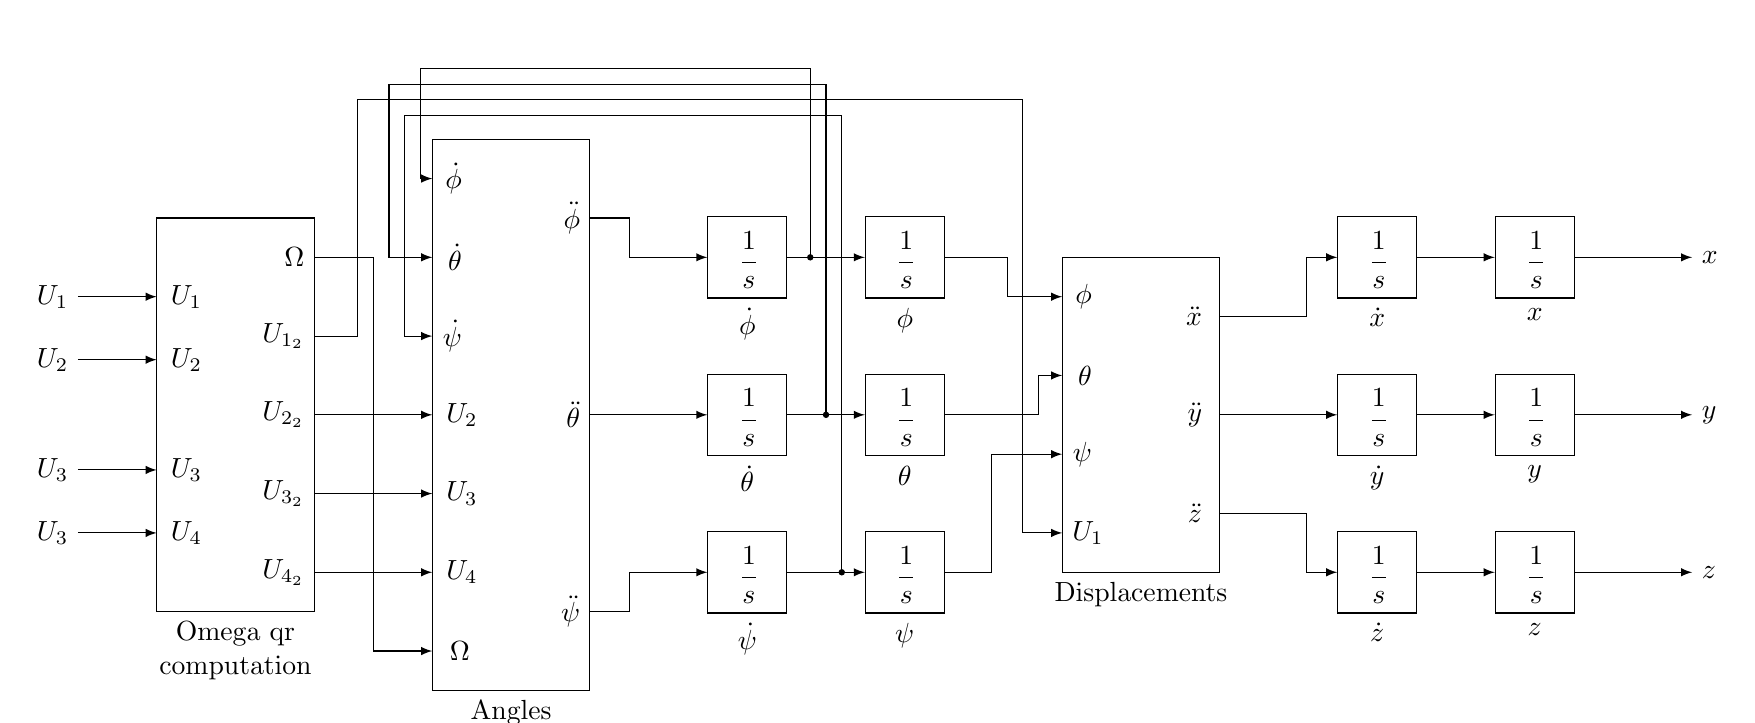
\begin{tikzpicture}
			
			%Initial links
			\draw[-latex] (-5.5,1.5) coordinate node[left]{$U_1$} -- (-4.5,1.5) coordinate;
			\draw[-latex] (-5.5,0.7) coordinate node[left]{$U_2$} -- (-4.5,0.7) coordinate;
			\draw[-latex] (-5.5,-0.7) coordinate node[left]{$U_3$} -- (-4.5,-0.7) coordinate;
			\draw[-latex] (-5.5,-1.5) coordinate node[left]{$U_3$} -- (-4.5,-1.5) coordinate;
			
			%Omega qr calculator block
			\node (omegaQRCalculator) at (-3.5,0) [draw, rectangle, minimum height=5cm, minimum 
			width=2cm, text centered, label={[align=center]below:Omega qr\\computation}]{};
			
			%Variables - omega qr calculator
			\draw (-3.8, 1.5) coordinate node[left]{$U_{1}$};
			\draw (-3.8, 0.7) coordinate node[left]{$U_{2}$};
			\draw (-3.8, -0.7) coordinate node[left]{$U_{3}$};
			\draw (-3.8, -1.5) coordinate node[left]{$U_{4}$};
			
			\draw (-2.5, 2.0) coordinate node[left]{$\Omega$};
			\draw (-2.5, 1.0) coordinate node[left]{$U_{1_{2}}$};
			\draw (-2.5, 0.0) coordinate node[left]{$U_{2_{2}}$};
			\draw (-2.5, -1.0) coordinate node[left]{$U_{3_{2}}$};
			\draw (-2.5, -2.0) coordinate node[left]{$U_{4_{2}}$};
			
			%Links between the omega and angles blocks
			\draw[-latex] (-2.5,2.0) coordinate -- (-1.75,2.0) coordinate -- (-1.75,-3.0) 
			coordinate -- (-1,-3.0) coordinate;
			\draw[-latex] (-2.5,1.0) coordinate -- (-1.95,1.0) coordinate -- (-1.95,4.0) coordinate 
			-- (6.5,4.0) coordinate -- (6.5,-1.5) coordinate -- (7,-1.5) coordinate;
			\draw[-latex] (-2.5,0.0) coordinate -- (-1,0.0) coordinate;
			\draw[-latex] (-2.5,-1.0) coordinate -- (-1,-1.0) coordinate;
			\draw[-latex] (-2.5,-2.0) coordinate -- (-1,-2.0) coordinate;
			
			%Angles block
			\node (anglesBlock) at (0,0) [draw, rectangle, minimum height=7cm, minimum width=2cm, 
			text centered, label={[align=center]below:Angles}]{};
			
			%Variables - angles
			\draw (-0.5,3.0) coordinate node[left]{$\dot{\phi}$};
			\draw (-0.5,2.0) coordinate node[left]{$\dot{\theta}$};
			\draw (-0.5,1.0) coordinate node[left]{$\dot{\psi}$};
			\draw (-0.3,0.0) coordinate node[left]{$U_2$};
			\draw (-0.3,-1.0) coordinate node[left]{$U_3$};
			\draw (-0.3,-2.0) coordinate node[left]{$U_4$};
			\draw (-0.4,-3.0) coordinate node[left]{$\Omega$};
			
			\draw (1.0, 2.5) coordinate node[left]{$\ddot{\phi}$};
			\draw (1.0, 0.0) coordinate node[left]{$\ddot{\theta}$};
			\draw (1.0, -2.5) coordinate node[left]{$\ddot{\psi}$};
			
			%First integrator block - angles
			\node (integrator1) at (3,0) [draw, rectangle, minimum height=1cm, minimum width=1cm, 
			text centered, label={[align=center]below:$\dot{\theta}$}]{$\cfrac{1}{s}$};
			\node (integrator2) at (3,2) [draw, rectangle, minimum height=1cm, minimum width=1cm, 
			text centered, label={[align=center]below:$\dot{\phi}$}]{$\cfrac{1}{s}$};
			\node (integrator3) at (3,-2) [draw, rectangle, minimum height=1cm, minimum width=1cm, 
			text centered, label={[align=center]below:$\dot{\psi}$}]{$\cfrac{1}{s}$};
			
			%Links between the angles and integrator blocks
			\draw[-latex] (1.0,2.5) coordinate -- (1.5,2.5) coordinate -- (1.5,2.0) coordinate -- 
			(integrator2.west);
			\draw[-latex] (1.0,0.0) coordinate -- (integrator1.west);
			\draw[-latex] (1.0,-2.5) coordinate -- (1.5,-2.5) coordinate -- (1.5,-2.0) coordinate 
			-- (integrator3.west);
			
			%Second integrators block - angles
			\node (integrator4) at (5,0) [draw, rectangle, minimum height=1cm, minimum width=1cm, 
			text centered, label={[align=center]below:$\theta$}]{$\cfrac{1}{s}$};
			\node (integrator5) at (5,2) [draw, rectangle, minimum height=1cm, minimum width=1cm, 
			text centered, label={[align=center]below:$\phi$}]{$\cfrac{1}{s}$};
			\node (integrator6) at (5,-2) [draw, rectangle, minimum height=1cm, minimum width=1cm, 
			text centered, label={[align=center]below:$\psi$}]{$\cfrac{1}{s}$};
			
			%Circle on the connection links
			\node[circle,draw,black,scale=0.2, fill=black] (A) at (4,0){};
			\node[circle,draw,black,scale=0.2, fill=black] (A) at (4.2,-2){};
			\node[circle,draw,black,scale=0.2, fill=black] (A) at (3.8,2){};
			
			%Links among blocks
			\draw[-latex] (4,0) coordinate -- (4,4.2) coordinate -- (-1.55,4.2) coordinate -- 
			(-1.55,2.0) coordinate -- (-1.0,2.0);
			\draw[-latex] (4.2,-2) coordinate -- (4.2,3.8) coordinate -- (-1.35,3.8) coordinate -- 
			(-1.35,1.0) coordinate -- (-1.0,1.0);
			\draw[-latex] (3.8,2) coordinate -- (3.8,4.4) coordinate -- (-1.15,4.4) coordinate -- 
			(-1.15,3.0) coordinate -- (-1.0,3.0);
			
			%Links among integrators blocks
			\draw[-latex] (integrator1.east) -- (integrator4.west);
			\draw[-latex] (integrator2.east) -- (integrator5.west);
			\draw[-latex] (integrator3.east) -- (integrator6.west);
			
			%Connection links between the integrators and displacement blocks
			\draw[-latex] (integrator5.east) -- (6.3,2) coordinate -- (6.3,1.5) coordinate -- 
			(7.0,1.5) coordinate;
			\draw[-latex] (integrator4.east) -- (6.7,0.0) coordinate -- (6.7,0.5) coordinate -- 
			(7.0,0.5) coordinate;
			\draw[-latex] (integrator6.east) -- (6.1,-2) coordinate -- (6.1,-0.5) coordinate -- 
			(7.0,-0.5) coordinate;
			
			%Displacement block
			\node (bloccoDisplacement) at (8,0) [draw, rectangle, minimum height=4cm, minimum 
			width=2cm, text centered, label={[align=center]below:Displacements}]{};
			
			%Variables - displacement
			\draw (7.5,1.5) coordinate node[left]{$\phi$};
			\draw (7.5,0.5) coordinate node[left]{$\theta$};
			\draw (7.5,-0.5) coordinate node[left]{$\psi$};
			\draw (7.65,-1.5) coordinate node[left]{$U_1$};
			
			\draw (8.9,1.25) coordinate node[left]{$\ddot{x}$};
			\draw (8.9,0.0) coordinate node[left]{$\ddot{y}$};
			\draw (8.9,-1.25) coordinate node[left]{$\ddot{z}$};
			
			%First integrators block - displacement
			\node (integrator7) at (11,0) [draw, rectangle, minimum height=1cm, minimum width=1cm, 
			text centered, label={[align=center]below:$\dot{y}$}]{$\cfrac{1}{s}$};
			\node (integrator8) at (11,2) [draw, rectangle, minimum height=1cm, minimum width=1cm, 
			text centered, label={[align=center]below:$\dot{x}$}]{$\cfrac{1}{s}$};
			\node (integrator9) at (11,-2) [draw, rectangle, minimum height=1cm, minimum width=1cm, 
			text centered, label={[align=center]below:$\dot{z}$}]{$\cfrac{1}{s}$};
			
			%Links for the displacement block
			\draw[-latex] (9,1.25) coordinate -- (10.1,1.25) coordinate -- (10.1,2) coordinate -- 
			(integrator8.west);
			\draw[-latex] (9,0.0) coordinate -- (integrator7.west);
			\draw[-latex] (9,-1.25) coordinate -- (10.1,-1.25) coordinate -- (10.1,-2) coordinate 
			-- (integrator9.west);
			
			%Second block of integrators - displacement
			\node (integrator10) at (13,0) [draw, rectangle, minimum height=1cm, minimum width=1cm, 
			text centered,label={[align=center]below:$y$}]{$\cfrac{1}{s}$};
			\node (integrator11) at (13,2) [draw, rectangle, minimum height=1cm, minimum width=1cm, 
			text centered,label={[align=center]below:$x$}]{$\cfrac{1}{s}$};
			\node (integrator12) at (13,-2) [draw, rectangle, minimum height=1cm, minimum 
			width=1cm, text centered,label={[align=center]below:$z$}]{$\cfrac{1}{s}$};
			
			%Connections between the two integrators blocks
			\draw[-latex] (integrator7.east) -- (integrator10.west);
			\draw[-latex] (integrator8.east) -- (integrator11.west);
			\draw[-latex] (integrator9.east) -- (integrator12.west);
			
			%Final interconnections
			\draw[-latex] (integrator10.east) -- (15,0) coordinate node[right]{$y$};
			\draw[-latex] (integrator11.east) -- (15,2) coordinate node[right]{$x$};
			\draw[-latex] (integrator12.east) -- (15,-2) coordinate node[right]{$z$};
			
			\end{tikzpicture}
		}
	\end{center}
	
\end{figure}

\section{Example \theblockDiagram}
\stepcounter{blockDiagram}

\begin{figure}[h]
	\begin{center}
		\scalebox{0.85}{
			
			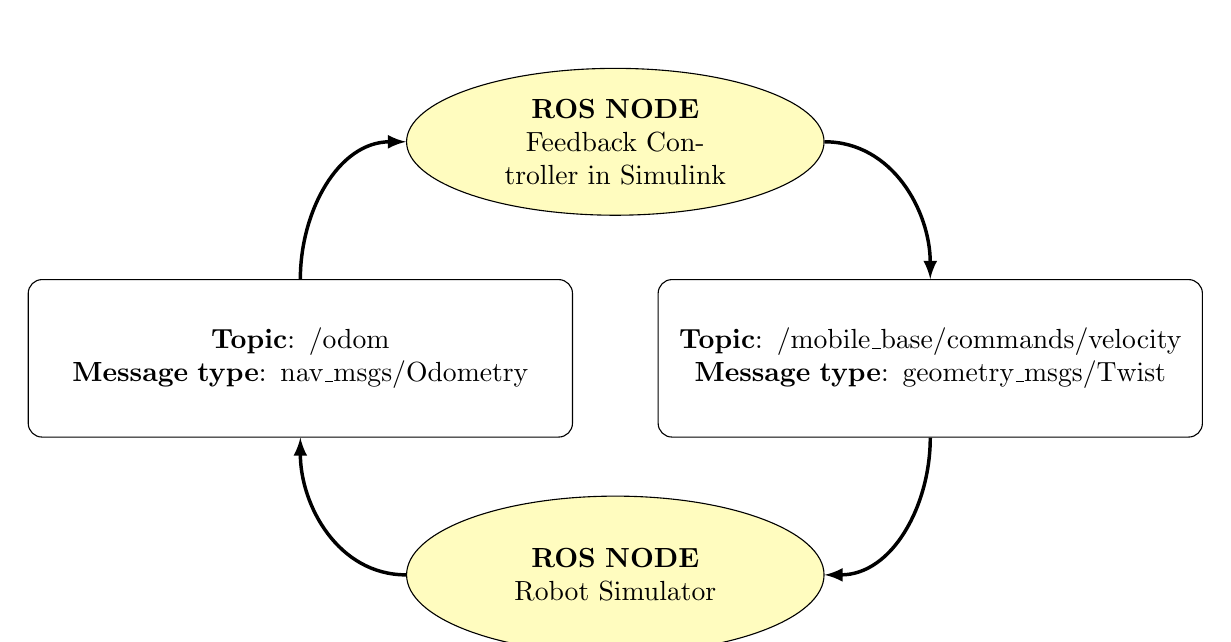
\begin{tikzpicture}
			\node (feedbackController) at (0,1.25) [draw, ellipse, text centered, minimum 
			height=1cm, fill=yellow!25, text width=10em]{\textbf{ROS NODE}\\Feedback Controller in 
			Simulink};
			\node (robotSimulator) at (0,-4.25) [draw, ellipse, text centered, minimum 
			height=2cm,fill=yellow!25, text width=10em]{\textbf{ROS NODE}\\Robot Simulator};
			
			\node (odom) at (-4,-1.5) [draw, rectangle, text centered, text width=19em, minimum 
			height=2cm, rounded corners=5pt]{\textbf{Topic}: /odom\\\textbf{Message type}: 
			nav\_msgs/Odometry};
			\node (mobileBase) at (4,-1.5) [draw, rectangle, text centered, text width=19em, 
			minimum height=2cm, rounded corners=5pt]{\textbf{Topic}: 
			/mobile\_base/commands/velocity\\\textbf{Message type}: geometry\_msgs/Twist};
			
			\draw[-latex, line width=1.25pt] (feedbackController) [out=0, in=90] to (mobileBase);
			\draw[-latex, line width=1.25pt] (mobileBase) [out=270, in=0] to (robotSimulator);
			\draw[-latex, line width=1.25pt] (robotSimulator) [out=180, in=270] to (odom);
			\draw[-latex, line width=1.25pt] (odom) [out=90, in=180] to (feedbackController); 
			
			\end{tikzpicture}
		}
	\end{center}
\end{figure}


\section{Example \theblockDiagram}
\stepcounter{blockDiagram}

\begin{figure}[h]
	\begin{center}
		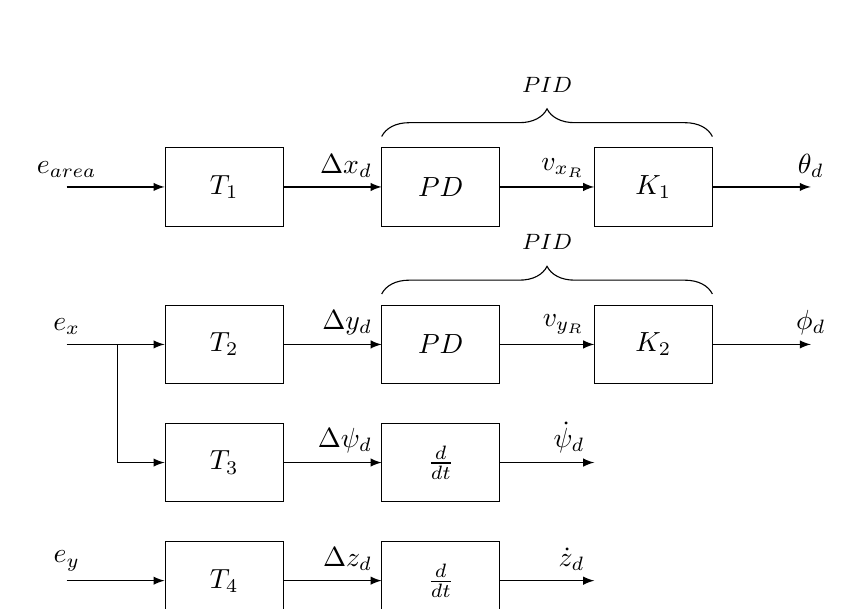
\begin{tikzpicture}
		
		%Nodes in the first part of the scheme
		\node (firstTransformation) at (-2,0.5) [draw, rectangle, minimum width=1.5cm, minimum 
		height=1cm, text centered]{$T_1$};
		
		\node (firstPD) at (0.75,0.5) [draw, text centered, minimum width=1.5cm, minimum 
		height=1cm]{$PD$};
		
		\node (firstK) at (3.45,0.5) [draw, text centered, minimum width=1.5cm, minimum 
		height=1cm]{$K_1$};
		
		\draw [decorate,decoration={brace, mirror, amplitude=10pt,raise=4pt},yshift=0pt]
		(4.2,1) -- (0,1) node [black,midway,yshift=0.8cm] {\footnotesize $PID$};
		
		%Links
		\draw[-latex] (-4,0.5) coordinate node[above]{$e_{area}$} -- (firstTransformation.west);
		
		\draw[-latex] (firstTransformation.east) -- (0,0.5) coordinate node[above left]{$\Delta 
		x_d$};
		
		\draw[-latex] (firstPD.east) -- (2.7,0.5) coordinate node[above left]{$v_{{x}_R}$};
		
		\draw[-latex] (firstK.east) -- (5.45,0.5) coordinate node[above]{$\theta_d$};
		
		
		%Nodes in the second part of the scheme
		\node (secondTransformation) at (-2,-1.5) [draw, rectangle, minimum width=1.5cm, minimum 
		height=1cm, text centered]{$T_2$};
		
		\node (secondPD) at (0.75,-1.5) [draw, text centered, minimum width=1.5cm, minimum 
		height=1cm]{$PD$};
		
		\node (secondK) at (3.45,-1.5) [draw, text centered, minimum width=1.5cm, minimum 
		height=1cm]{$K_2$};
		
		\draw [decorate,decoration={brace, mirror, amplitude=10pt,raise=4pt},yshift=0pt]
		(4.2,-1.0) -- (0,-1.0) node [black,midway,yshift=0.8cm] {\footnotesize
			$PID$};
		
		%Links among blocks
		\draw[-latex] (-4,-1.5) coordinate node[above]{$e_x$} -- (secondTransformation.west);
		
		\draw[-latex] (secondTransformation.east) -- (0,-1.5) coordinate node[above left]{$\Delta 
		y_d$};
		
		\draw[-latex] (secondPD.east) -- (2.7,-1.5) coordinate node[above left]{$v_{{y}_R}$};
		
		\draw[-latex] (secondK.east) -- (5.45,-1.5) coordinate node[above]{$\phi_d$};
		
		
		%Nodes in the third part of the scheme
		\node (thirdTransformation) at (-2,-3.0) [draw, rectangle, minimum width=1.5cm, minimum 
		height=1cm, text centered]{$T_3$};
		
		\node (thirdPD) at (0.75,-3.0) [draw, text centered, minimum width=1.5cm, minimum 
		height=1cm]{$\frac{d}{dt}$};
		
		%Links among blocks
		\draw[-latex] (-3.35, -1.5) coordinate --  (-3.35,-3.0) coordinate -- 
		(thirdTransformation.west);
		
		\draw[-latex] (thirdTransformation.east) -- (0,-3.0) coordinate node[above left]{$\Delta 
		\psi_d$};
		
		\draw[-latex] (thirdPD.east) -- (2.7,-3.0) coordinate node[above left]{$\dot{\psi}_d$};
		
		
		%Nodes of the fourth part of the scheme
		\node (fourthTransformation) at (-2,-4.5) [draw, rectangle, minimum width=1.5cm, minimum 
		height=1cm, text centered]{$T_4$};
		
		\node (fourthPD) at (0.75,-4.5) [draw, text centered, minimum width=1.5cm, minimum 
		height=1cm]{$\frac{d}{dt}$};
		
		%Links among blocks
		\draw[-latex] (-4,-4.5) coordinate node[above]{$e_y$} -- (fourthTransformation.west);
		
		\draw[-latex] (fourthTransformation.east) -- (0,-4.5) coordinate node[above left]{$\Delta 
		z_d$};
		
		\draw[-latex] (fourthPD.east) -- (2.7,-4.5) coordinate node[above left]{$\dot{z}_d$};
		
		
		\end{tikzpicture}
	\end{center}
	
\end{figure}

\newpage

\section{Example \theblockDiagram}
\stepcounter{blockDiagram}

\begin{figure}[h]
	\begin{center}
		\scalebox{1}{
			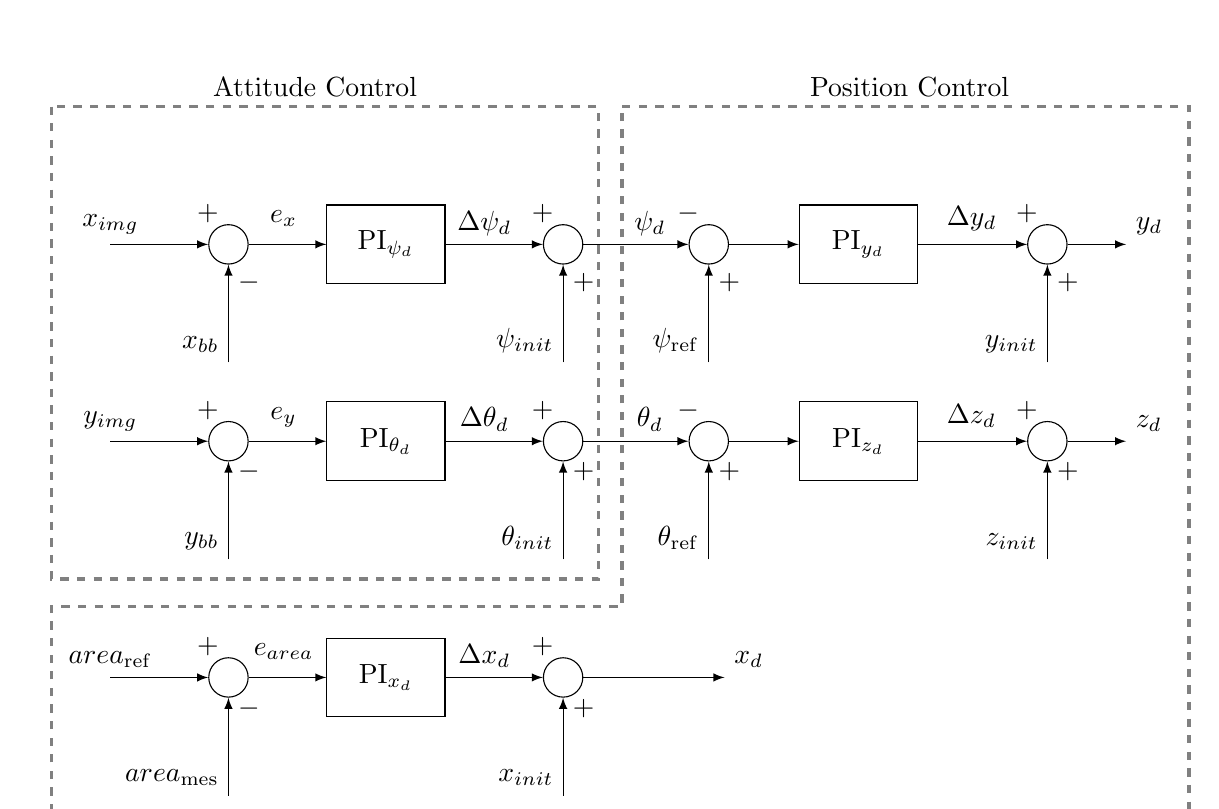
\begin{tikzpicture}
			
			%Attitude controller
			\node (attitudeController) at (-3.40,-1.25) [rectangle, label=Attitude Control, text 
			centered, minimum height=6cm, minimum width=7.3cm]{};
			
			\draw[dashed, gray, line width=1.25pt] (-6.75,1.75) coordinate -- (-6.75,-4.25) 
			coordinate -- (0.2,-4.25) coordinate -- (0.2,1.75) coordinate -- (-6.75,1.75) 
			coordinate;
			
			%Position controller
			\draw[dashed, gray, line width=1.25pt] (0.5, 1.75) coordinate -- (7.7, 1.75) coordinate 
			-- (7.7, -7.3) coordinate --  (-6.75,-7.3) coordinate -- (-6.75,-4.6) coordinate --  
			(0.5,-4.6) coordinate -- (0.5,1.75) coordinate;
			
			\node (positionController) at (4.15,-1.25) [label=Position Control, text centered, 
			minimum width=2.65cm, minimum height=6cm, rectangle]{};
			
			%Blocks in the first part of the scheme
			\node (adder1) at (-4.5,0) [draw, circle, text centered, minimum size=0.5cm]{};
			
			\node (pi1) at (-2.5,0) [draw, rectangle, text centered, minimum height=1.0cm, minimum 
			width=1.5cm]{$\text{PI}_{\psi_d}$};
			
			\node (adder2) at (-0.25,0) [draw, circle, text centered, minimum size=0.5cm]{};
			
			\node (adder20) at (1.6,0) [draw, circle, text centered, minimum size=0.5cm]{};
			
			\node (pi2) at (3.5,0) [draw, rectangle, text centered, minimum height=1cm, minimum 
			width=1.5cm]{$\text{PI}_{y_d}$};
			
			\node (adder6) at (5.9,0) [draw, circle, text centered, minimum size=0.5cm]{};
			
			%Links among blocks
			\draw[-latex] (-6.0,0) coordinate node[above]{$x_{img}$} -- (adder1.west);
			\draw[-latex] (-4.5,-1.5) coordinate node[above left]{$x_{bb}$} -- (adder1.south);
			
			\draw[-latex] (adder1.east) -- (pi1.west);
			\draw[-latex] (pi1.east) -- (adder2.west);
			
			\draw[-latex] (-0.25,-1.5) coordinate node[above left]{$\psi_{init}$}-- (adder2.south);
			
			\draw[-latex] (1.6,-1.5) coordinate node[above left]{$\psi_\mathrm{ref}$} -- 
			(adder20.south);
			
			\draw[-latex] (adder2.east) -- (adder20.west);
			\draw[-latex] (adder20.east) -- (pi2.west);
			\draw[-latex] (pi2.east) -- (adder6.west);
			\draw (4.5,0.05) node[above right]{$\Delta y_d$};
			
			\draw[-latex] (5.9,-1.5) coordinate node[above left]{$y_{init}$} -- (adder6.south);
			\draw[-latex] (adder6.east) -- (6.9,0) coordinate node[above right]{$y_d$};
			
			%Signs
			\draw (-4.5,0.15) coordinate node[above left]{$+$};
			\draw (-4.5,-0.25) coordinate node[below right]{$-$};
			
			\draw (-0.25,0.15) coordinate node[above left]{$+$};
			\draw (-0.25,-0.25) coordinate node[below right]{$+$};
			
			\draw (1.6,0.15) coordinate node[above left]{$-$};
			\draw (1.6,-0.25) coordinate node[below right]{$+$};
			
			\draw (5.9,0.15) coordinate node[above left]{$+$};
			\draw (5.9,-0.25) coordinate node[below right]{$+$};
			
			%Errors
			\draw (-3.8,0.55) coordinate node[below]{$e_x$};
			\draw (-1.25,0.55) coordinate node[below]{$\Delta \psi_d$};
			\draw (0.85,0.55) coordinate node[below]{$\psi_d$};
			
			
			%Blocks in the second part of the scheme
			\node (adder3) at (-4.5,-2.5) [draw, circle, text centered, minimum size=0.5cm]{};
			
			\node (pi3) at (-2.5,-2.5) [draw, rectangle, text centered, minimum height=1.0cm, 
			minimum width=1.5cm]{$\text{PI}_{\theta_d}$};
			
			\node (adder4) at (-0.25,-2.5) [draw, circle, text centered, minimum size=0.5cm]{};
			
			\node (adder50) at (1.6,-2.5) [draw, circle, text centered, minimum size=0.5cm]{};
			
			\node (pi4) at (3.5,-2.5) [draw, rectangle, text centered, minimum height=1cm, minimum 
			width=1.5cm]{$\text{PI}_{z_d}$};
			
			\node (adder7) at (5.9,-2.5) [draw, circle, text centered, minimum size=0.5cm]{}; 
			
			%Links among blocks
			\draw[-latex] (-6.0,-2.5) coordinate node[above]{$y_{img}$} -- (adder3.west);
			\draw[-latex] (-4.5,-4.0) coordinate node[above left]{$y_{bb}$} -- (adder3.south);
			
			\draw[-latex] (adder3.east) -- (pi3.west);
			\draw[-latex] (pi3.east) -- (adder4.west);
			
			\draw[-latex] (-0.25,-4.0) coordinate node[above left]{$\theta_{init}$} -- 
			(adder4.south);
			
			\draw[-latex] (1.6,-4.0) coordinate node[above left]{$\theta_\mathrm{ref}$} -- 
			(adder50.south);
			
			\draw[-latex] (adder4.east) -- (adder50.west);
			\draw[-latex] (adder50.east) -- (pi4.west);
			\draw[-latex] (pi4.east) -- (adder7.west); 
			\draw (4.5,-2.45) coordinate node[above right]{$\Delta z_d$};
			
			\draw[-latex] (5.9,-4.0) node[above left]{$z_{init}$} -- (adder7.south);
			
			\draw[-latex] (adder7.east) -- (6.9,-2.5) coordinate node[above right]{$z_d$};
			
			%Sings
			\draw (-4.5,-2.35) coordinate node[above left]{$+$};
			\draw (-4.5,-2.65) coordinate node[below right]{$-$};
			
			\draw (-0.25,-2.35) coordinate node[above left]{$+$};
			\draw (-0.25,-2.65) coordinate node[below right]{$+$};
			
			\draw (1.6,-2.35) coordinate node[above left]{$-$};
			\draw (1.6,-2.65) coordinate node[below right]{$+$};
			
			\draw (5.9,-2.35) coordinate node[above left]{$+$};
			\draw (5.9,-2.65) coordinate node[below right]{$+$};
			
			%Errors
			\draw (-3.8,-1.95) coordinate node[below]{$e_y$};
			\draw (-1.25,-1.95) coordinate node[below]{$\Delta \theta_d$};
			\draw (0.85,-1.95) coordinate node[below]{$\theta_d$};
			
			%Blocks in the third part of the scheme
			\node (adder5) at (-4.5,-5.5) [draw, circle, text centered, minimum size=0.5cm]{};
			
			\node (pi5) at (-2.5,-5.5) [draw, rectangle, text centered, minimum height=1.0cm, 
			minimum width=1.5cm]{$\text{PI}_{x_d}$};
			
			\node (adder8) at (-0.25,-5.5) [draw, circle, text centered, minimum size=0.5cm]{};
			
			%Links
			\draw[-latex] (-6.0,-5.5) coordinate node[above]{$area_{\mathrm{ref}}$} -- 
			(adder5.west);
			\draw[-latex] (-4.5,-7.0) coordinate node[above left]{$area_{\mathrm{mes}}$} -- 
			(adder5.south);
			
			\draw[-latex] (adder5.east) -- (pi5.west);
			
			\draw[-latex] (pi5.east) -- (adder8.west);
			\draw (-1.25,-5.5) coordinate node[above]{$\Delta x_d$};
			
			\draw[-latex] (-0.25,-7.0) coordinate node[above left]{$x_{init}$} -- (adder8.south);
			
			%Signs
			\draw (-4.5,-5.35) coordinate node[above left]{$+$};
			\draw (-4.5,-5.65) coordinate node[below right]{$-$};
			
			\draw (-0.25,-5.35) coordinate node[above left]{$+$};
			\draw (-0.25,-5.65) coordinate node[below right]{$+$};
			
			\draw[-latex] (adder8.east) -- (1.8,-5.5) coordinate node[above right]{$x_d$};
			
			%Errors
			\draw (-3.8,-4.95) coordinate node[below]{$e_{area}$};
			
			
			\end{tikzpicture}
		}
	\end{center}

\end{figure}

\section{Example \theblockDiagram}
\stepcounter{blockDiagram}

\begin{figure}[h]
	\begin{center}
		\scalebox{1}{
			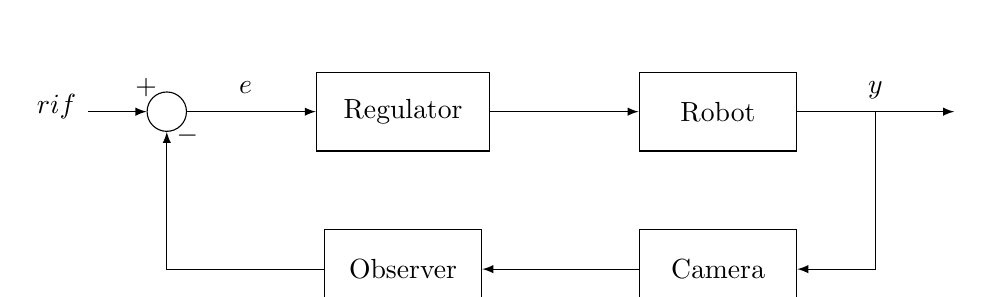
\begin{tikzpicture}[node distance=2cm]
			
			%Nodes
			\node (adder) at (0,0) [draw, circle, text centered, minimum size=0.5cm]{};
			
			\node (regulator) at (3,0) [draw, rectangle, text centered, minimum width=2.2cm, 
			minimum height=1cm]{Regulator};
			
			\node (robot) at (7,0) [draw, rectangle, text centered, minimum width=2cm, minimum 
			height=1cm]{Robot};
			
			\node (camera) at (7,-2) [draw, rectangle, text centered, minimum width=2cm, minimum 
			height=1cm]{Camera};
			
			\node (observer) at (3,-2) [draw, rectangle, text centered, minimum width=2cm, minimum 
			height=1cm]{Observer};
			
			%Links
			\draw[-latex] (adder) --  (regulator);
			\draw[-latex] (camera) -- (observer);
			\draw[-latex] (regulator) -- (robot);
			\draw[-latex] (observer.west) -- (0,-2) coordinate -- (adder.south);
			\draw[-latex] (robot.east) -- (10,0) coordinate;
			\draw[-latex] (9,0) coordinate -- (9,-2) coordinate -- (camera.east);
			\draw[-latex] (-1,0) coordinate -- (adder.west);
			
			%Variables
			\draw (9, 0.5) coordinate node[below]{$y$};
			\draw (1, 0.5) coordinate node[below]{$e$};
			\draw (-1.4,0.35) coordinate node[below]{$rif$};
			\draw (0,0.55) coordinate node[below left]{$+$};
			\draw (0,-0.55) coordinate node[above right]{$-$};
			
			\end{tikzpicture}
		}
	\end{center}
\end{figure}

\newpage


\section{Example \theblockDiagram}
\stepcounter{blockDiagram}

\begin{figure}[h]
	\begin{center}
		\scalebox{0.72}{
			\begin{tikzpicture}
			
			%Yaw angle
			\node (yawAngle) at (0,0) [draw, rectangle, minimum height=2cm, minimum width=2cm, text 
			centered]{};
			\draw (1,1) coordinate -- (1.2,1.2) coordinate;
			\draw (1,-1) coordinate -- (1.2,-1.2) coordinate;
			\draw (1.2,-1.2) coordinate -- (1.2,1.2) coordinate;
			
			%Drawing the angle
			\draw (1.8,0) coordinate -- (2.2,0) coordinate;
			\draw[-latex, line width=1.0pt] (2.0,0) coordinate -- (2.0, -1) coordinate node[above 
			right]{$\psi_d$};
			
			%Reference system
			\draw[-latex] (-4,2) coordinate -- (-4,-1) coordinate node[above left]{$z$};
			\draw[-latex] (-4,2) coordinate -- (-2,2) coordinate node[above]{$x$};
			\node (circle) at (-4,2) [circle, draw, minimum size=0.5cm]{};
			\node[circle,draw,black,scale=0.2, fill=black] (A) at (-4,2) {};
			\draw (-4.25,2) coordinate node[above left]{$y$};
			
			%Dividing line among schems
			\draw[dashed, draw=gray] (-6,-2) coordinate -- (6,-2) coordinate;
			
			%Roll angle
			\node (rollAngle) at (0,-5) [draw, rectangle, minimum height=2cm, minimum width=2cm, 
			text centered]{};
			\draw (1,-4) coordinate -- (1.2,-3.8) coordinate;
			\draw (1,-6) coordinate -- (1.2,-6.2) coordinate;
			\draw (1.2,-3.8) coordinate -- (1.2,-6.2) coordinate;
			
			%Roll angle drawing
			\draw (1.8,-5) coordinate -- (2.2,-5) coordinate;
			\draw[-latex, line width=1.0pt] (2.0,-5) coordinate -- (2.0, -6) coordinate node[above 
			right]{$\phi_d$};
			
			%Reference system
			\draw[-latex] (-4,-3) coordinate -- (-2,-3) coordinate node[above]{$x$};
			\draw[-latex] (-4,-3) coordinate -- (-4,-6) coordinate node[above left]{$z$};
			\node (circle) at (-4,-3) [circle, draw, minimum size=0.5cm]{};
			\node[circle,draw,black,scale=0.2, fill=black] (A) at (-4,-3) {};
			\draw (-4.25,-3) coordinate node[above left]{$y$};
			
			%Diving line among schemes
			\draw[dashed, draw=gray] (-6,-7) coordinate -- (6,-7) coordinate;
			
			%Pitch angle
			\node (rollAngle) at (0,-9) [draw, rectangle, minimum height=2cm, minimum width=2cm, 
			text centered]{};
			\draw (1,-8) coordinate -- (1.2,-7.8) coordinate;
			\draw (1,-10) coordinate -- (1.2,-10.2) coordinate;
			\draw (1.2,-7.8) coordinate -- (1.2,-10.2) coordinate;
			
			%Drawing the angle
			\draw (0,-10.8) coordinate -- (0,-11.2) coordinate;
			\draw[-latex, line width=1.0pt] (0,-11) coordinate -- (1.0, -11) coordinate node[above 
			right]{$\theta_d$};
			
			%Reference system
			\draw[-latex] (-4,-10.5) coordinate -- (-2,-10.5) coordinate node[above]{$x$};
			\draw[-latex] (-4,-10.5) coordinate -- (-4,-8) coordinate node[above left]{$y$};
			\node (circle) at (-4,-10.5) [circle, draw, minimum size=0.5cm]{};
			\node[circle,draw,black,scale=0.2, fill=black] (A) at (-4,-10.5) {};
			\draw (-4.25,-10.5) coordinate node[above left]{$z$};
			
			
			\end{tikzpicture}
		}
	\end{center}

\end{figure}

\section{Example \theblockDiagram}
\stepcounter{blockDiagram}

\begin{figure}[h]
	\begin{center}
		\scalebox{0.95}{
		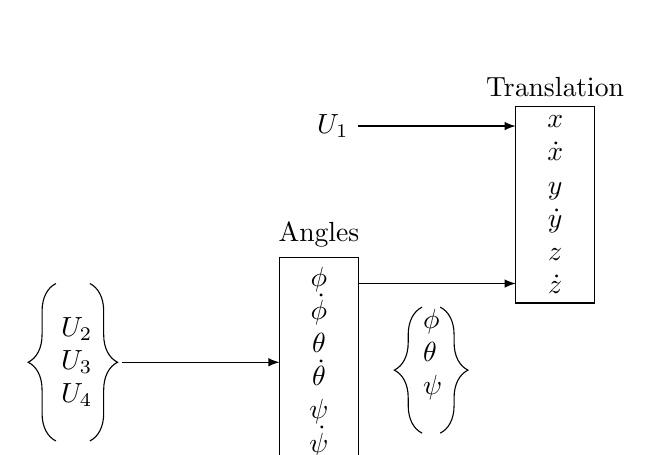
\begin{tikzpicture}
		
		%Drawing first rectangle
		\node (firstRectangle) at (0,0) [draw, rectangle, text centered, text width=1em, minimum 
		width=1cm, minimum height=2cm, label={Angles}]{$\phi$ \\ $\dot{\phi}$ \\ 
		$\theta$ \\ $\dot{\theta}$ \\ $\psi$ \\ $\dot{\psi}$};
		
		%Drawing second rectangle
		\node (secondRectangle) at (3,2) [draw, rectangle, text centered, text width=1em, minimum 
		width=1cm, minimum height=2cm, label={Translation}]{$x$ \\ $\dot{x}$ \\ $y$ \\ 
		$\dot{y}$ \\ $z$ \\ $\dot{z}$};
		
		%First arrow
		\draw[-latex] (0.5,1) coordinate -- (2.5,1) coordinate;
		\draw (1.5,0.8) coordinate node[below, text width=1em]{$\phi$ \\ $\theta$ \\ $\psi$};
		\draw [decorate,decoration={brace,amplitude=10pt,mirror,raise=4pt},yshift=0pt]
		(1.45,0.7) -- (1.45,-0.9) node [black,midway,xshift=0.8cm] {};
		\draw [decorate,decoration={brace,amplitude=10pt,raise=4pt},yshift=0pt]
		(1.40,0.7) -- (1.40,-0.9) node [black,midway,xshift=0.8cm] {};
		
		%Second arrow
		\draw[latex-] (-0.5,0) coordinate -- (-2.5,0) coordinate;
		\draw (-2.8,0) coordinate node[left, text width=1em]{$U_2$ \\ $U_3$ \\ $U_4$};
		\draw [decorate,decoration={brace,amplitude=10pt,mirror,raise=4pt},yshift=0pt]
		(-3.2,1) -- (-3.2,-1) node [black,midway,xshift=0.8cm] {};
		\draw [decorate,decoration={brace,amplitude=10pt,raise=4pt},yshift=0pt]
		(-3.05,1) -- (-3.05,-1) node [black,midway,xshift=0.8cm] {};
		
		%Third arrow
		\draw[-latex] (0.5,3) coordinate -- (2.5,3) coordinate;
		\draw (0.5,3) coordinate node[left]{$U_1$};
		
		\end{tikzpicture}
	}
	\end{center}

\end{figure}

\newpage

\section{Example \theblockDiagram}
\stepcounter{blockDiagram}

\begin{figure}[h]
	\begin{center}
			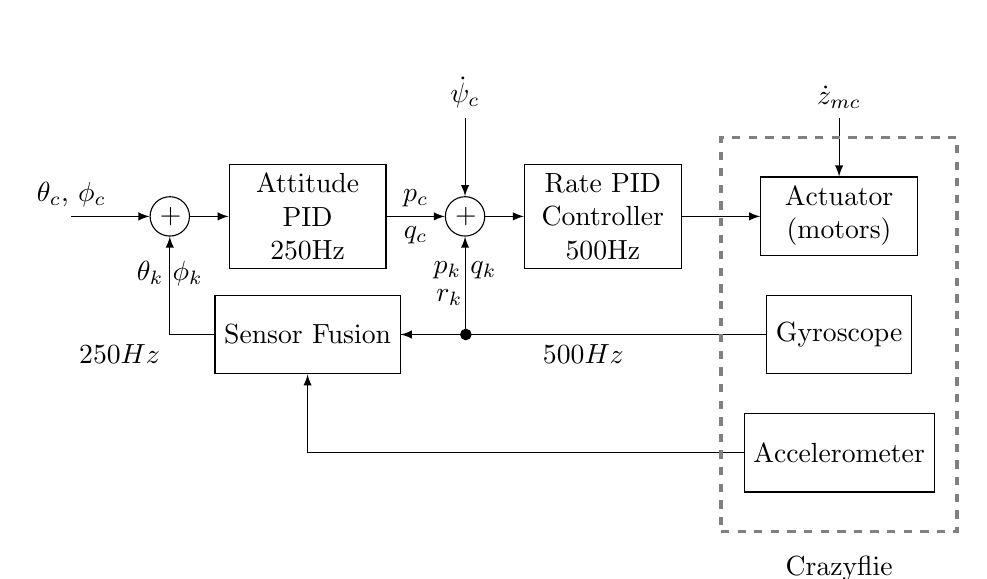
\begin{tikzpicture}
			
			%Blocks of the scheme
			\node (attitudePID) at (3.5,0) [draw, rectangle, minimum width=1cm, minimum height=1cm, 
			text centered, text width=5em]{Attitude PID\\250Hz};
			\node (ratePID) at (7.25,0) [draw, rectangle, minimum width=1cm, minimum height=1cm, 
			text centered, text width=5em]{Rate PID\\Controller\\500Hz};
			\node (actuators) at (10.25,0) [draw, rectangle, minimum width=1cm, minimum height=1cm, 
			text centered, text width=5em]{Actuator\\(motors)};
			\node (gyroscope) at (10.25,-1.5) [draw, rectangle, minimum width=1cm, minimum 
			height=1cm, text centered]{Gyroscope};
			\node (accelerometer) at (10.25,-3) [draw, rectangle, minimum width=1cm, minimum 
			height=1cm, text centered]{Accelerometer};
			\node (sensorFusion) at (3.5,-1.5) [draw, rectangle, minimum width=1cm, minimum 
			height=1cm, text centered]{Sensor Fusion};
			
			%Adders
			\node (adder1) at (1.75,0) [draw, circle, text centered, minimum size=0.5cm]{};
			\node (adder2) at (5.5,0) [draw, circle, text centered, minimum size=0.5cm]{};
			
			%Bubblies
			\node (coordinates1) at (5.51,-1.5) [circle, draw, scale=0.4, fill=black]{};
			
			%Linx
			\draw[-latex] (0.5,0) coordinate node[above]{$\theta_c$, $\phi_c$} -- (adder1);
			\draw[-latex] (adder1)   -- (attitudePID);
			\draw[-latex] (attitudePID) -- node[above]{$p_c$} node[below]{$q_c$} (adder2);
			\draw[-latex] (adder2) -- (ratePID);
			\draw[-latex] (ratePID) -- (actuators);
			\draw[-latex] (gyroscope) -- node[below]{$500Hz$} (sensorFusion);
			\draw[-latex] (accelerometer) -| (sensorFusion);
			\draw[-latex] (sensorFusion) -| (adder2);
			\draw[-latex] (sensorFusion) -| node[below left]{$250Hz$} (adder1);
			\draw[-latex] (5.5,1.25) coordinate node[above]{$\dot{\psi}_c$} -- (adder2);
			\draw[-latex] (10.25,1.25) coordinate node[above]{$\dot{z}_{mc}$} -- (actuators);
			
			%Senros fusion's outputs
			\draw (1.75,-0.45) coordinate node[below]{$\theta_k$ $\phi_k$};
			\draw (5.5,-0.45) coordinate node[below]{$p_k$ $q_k$};
			\draw (5.3,-0.8) coordinate node[below]{$r_k$};
			
			%Signs
			\draw (1.5,0) coordinate node[right]{$+$};
			\draw (5.25,0) coordinate node[right]{$+$};
			
			%Comments
			\node (Crazyflie) at (10.25,-1.5) [dashed, gray, rectangle, minimum width=3cm, 
			minimum height=5cm, draw, line width=1.25pt]{};
			\draw (10.25,-4.75) coordinate node[above]{Crazyflie};
			
			\end{tikzpicture}
	\end{center}
\end{figure}

\section{Example \theblockDiagram}
\stepcounter{blockDiagram}

\begin{figure}[h]
	\begin{center}
			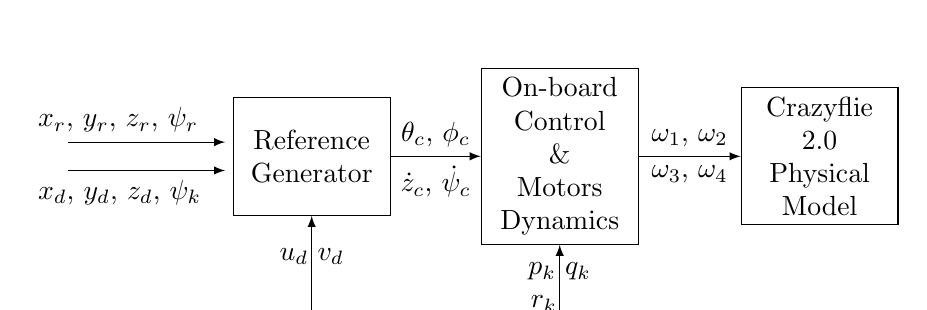
\begin{tikzpicture}
			
			%Blocks
			\node (ReferenceGenerator) at (-2.1,0) [draw, rectangle, minimum height=1.5cm, minimum 
			width=1cm, text centered, text width=5em]{Reference\\Generator};
			
			\node (OnboardCrazyflie) at (1.05,0) [draw, rectangle, minimum height=1.5cm, minimum 
			width=1cm, text centered, text width=5em]{On-board\\Control \\\& \\Motors Dynamics};
			
			\node (Crazyflie) at (4.35,0) [draw, rectangle, minimum height=1.5cm, minimum 
			width=1cm, text centered, text width=5em]{Crazyflie 2.0\\ Physical Model};
			
			%Links
			\draw[-latex] (ReferenceGenerator)  -- node[above]{$\theta_c$, $\phi_c$} 
			node[below]{$\dot{z}_c$, $\dot{\psi}_c$} (OnboardCrazyflie) ;
			\draw[-latex] (OnboardCrazyflie) -- node[above]{$\omega_1$, $\omega_2$} 
			node[below]{$\omega_3$, $\omega_4$}(Crazyflie);
			\draw[-latex] (-5.2,0.18)  -- (-3.2,0.18);
			\draw[-latex] (-5.2,-0.18) -- (-3.2,-0.18);
			\draw[-latex] (-2.1,-2.1) coordinate -- (ReferenceGenerator);
			\draw[-latex] (1.05,-2.1) coordinate -- (OnboardCrazyflie);
			\draw (0.85,-1.65) coordinate node[below]{$r_k$};
			
			%Variables
			\draw (-5.7,0.18) node[above right]{$x_r$, $y_r$, $z_r$, $\psi_r$};
			\draw (-5.7,-0.18) node[below right]{$x_d$, $y_d$, $z_d$, $\psi_k$};
			\draw (1.05,-1.7) node[above]{$p_k$ $q_k$};
			\draw (-2.1,-1.5) node[above]{$u_d$ $v_d$};
			
			\end{tikzpicture}
	\end{center}
\end{figure}


\section{Example \theblockDiagram}
\stepcounter{blockDiagram}

\begin{figure}[h]
	\begin{center}
		\scalebox{0.825}{
		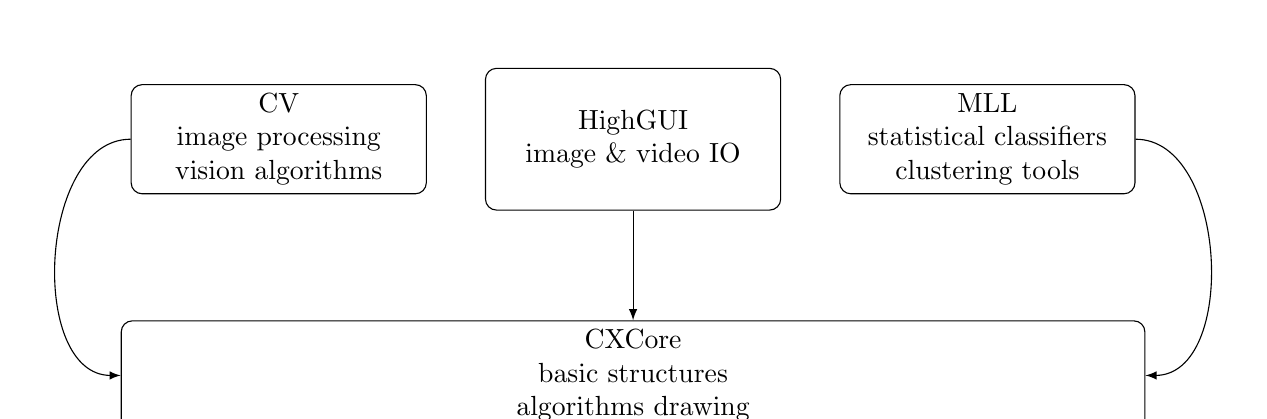
\begin{tikzpicture}
		
		%Nodes
		\node (highGUI) at (0,0) [rectangle, draw, minimum width=2cm, minimum height=1.8cm, 
		align=center, text width=10em, rounded corners]{HighGUI \\ image \& video IO};
		
		\node (CV) at (-4.5,0) [rectangle, draw, minimum width=2cm, minimum height=1cm, 
		align=center, text width=10em, rounded corners]{CV \\ image processing \\ vision 
		algorithms};
		
		\node (MLL) at (4.5,0) [rectangle, draw, minimum width=2cm, minimum height=1cm, 
		align=center, text width=10em, rounded corners]{MLL \\ statistical classifiers \\ 
		clustering tools};
		
		\node (CXCORE) at (0,-3) [rectangle, draw, minimum width=13cm, minimum height=1cm, 
		align=center, text width=10em, rounded corners]{CXCore \\ basic structures \\ algorithms 
		drawing};
		
		%Links
		\draw[-latex] (CV) to [out=180, in=180] (CXCORE);
		\draw[-latex] (highGUI.south) -- (CXCORE.90);
		\draw[-latex] (MLL) to [out=0, in=0] (CXCORE);
		
		\end{tikzpicture}
	}
	\end{center}

\end{figure}

\newpage


\section{Example \theblockDiagram}
\stepcounter{blockDiagram}

\begin{figure}[h]
	\begin{center}
		\scalebox{1}{
			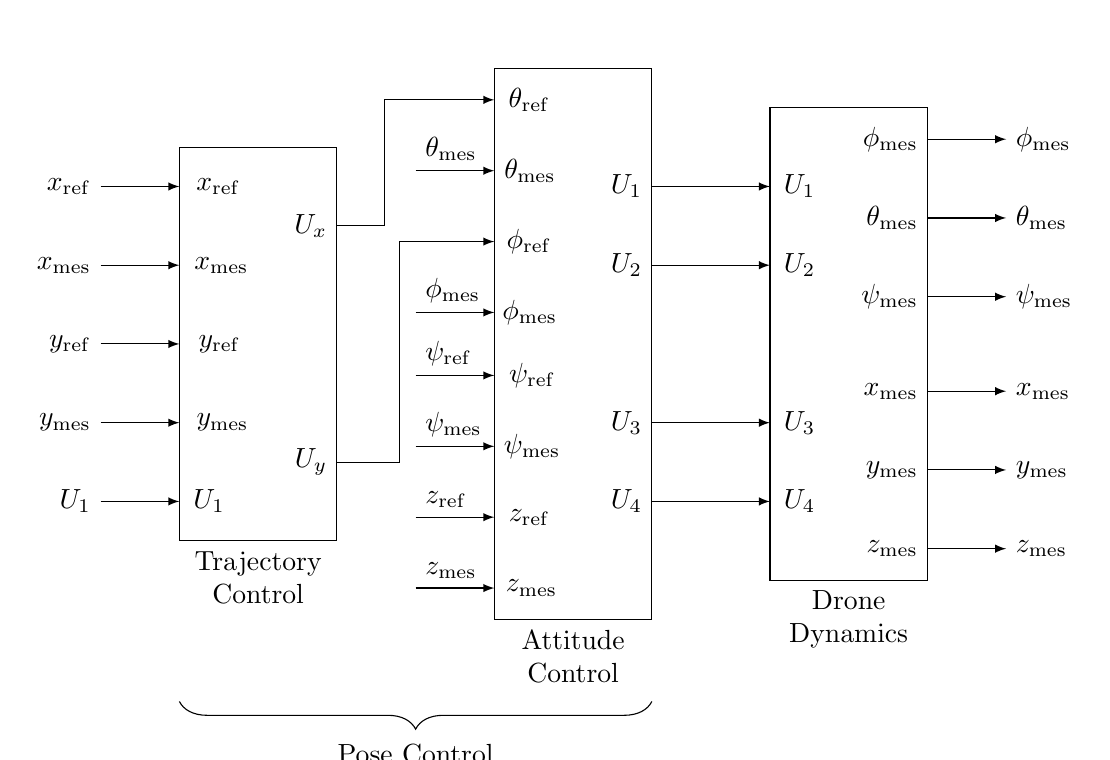
\begin{tikzpicture}
			
			%Trajectory controller
			\node (trajectoryController) at (-4,0) [draw, rectangle, minimum width=2cm, minimum 
			height=5cm, text centered, label={[align=center]below:Trajectory\\ Control}]{};
			
			%Variables
			\draw (-4.1,2.0) coordinate node[left]{$x_\mathrm{ref}$};
			\draw (-4.0,1.0) coordinate node[left]{$x_{\mathrm{mes}}$};
			\draw (-4.1,0.0) coordinate node[left]{$y_\mathrm{ref}$};
			\draw (-4.0,-1.0) coordinate node[left]{$y_{\mathrm{mes}}$};
			\draw (-4.3,-2.0) coordinate node[left]{$U_1$};
			
			\draw (-3.0,1.5) coordinate node[left]{$U_x$};
			\draw (-3.0,-1.5) coordinate node[left]{$U_y$};
			
			%Links
			\draw[-latex] (-6,2.0) coordinate node[left]{$x_\mathrm{ref}$} -- (-5,2.0) coordinate;
			\draw[-latex] (-6,1.0) coordinate node[left]{$x_{\mathrm{mes}}$} -- (-5,1.0) coordinate;
			\draw[-latex] (-6,0.0) coordinate node[left]{$y_\mathrm{ref}$} -- (-5,0.0) coordinate;
			\draw[-latex] (-6,-1.0) coordinate node[left]{$y_{\mathrm{mes}}$} -- (-5,-1.0) 
			coordinate;
			\draw[-latex] (-6,-2.0) coordinate node[left]{$U_1$} -- (-5,-2.0) coordinate; 
			
			
			%Attitude controller
			\node (attitudeController) at (0,0) [draw, rectangle, minimum width=2cm, minimum 
			height=7cm, text centered, label={[align=center]below:Attitude\\ Control}]{};
			
			%Curly brackets
			\draw [decorate,decoration={brace,mirror, amplitude=10pt,raise=4pt},yshift=0pt]
			(-5,-4.4) -- (1,-4.4) node [black,midway,xshift=0.0cm,yshift=-0.8cm] {Pose Control};
			
			%Variables
			\draw (-0.17,3.1) node[left]{$\theta_\mathrm{ref}$};
			\draw (-0.1,2.2) node[left]{$\theta_{\mathrm{mes}}$};
			\draw (-0.15,1.3) node[left]{$\phi_\mathrm{ref}$};
			\draw (-0.08,0.4) node[left]{$\phi_{\mathrm{mes}}$};
			\draw (-0.1,-0.4) node[left]{$\psi_\mathrm{ref}$};
			\draw (-0.04,-1.3) node[left]{$\psi_{\mathrm{mes}}$};
			\draw (-0.17,-2.2) node[left]{$z_\mathrm{ref}$};
			\draw (-0.08,-3.1) node[left]{$z_{\mathrm{mes}}$};
			
			\draw (1.0,2) node[left]{$U_1$};
			\draw (1.0,1) node[left]{$U_2$};
			\draw (1.0,-1) node[left]{$U_3$};
			\draw (1.0,-2) node[left]{$U_4$};
			
			%Links
			\draw[-latex] (-3.0,1.5) coordinate -- (-2.4,1.5) coordinate -- (-2.4,3.1) coordinate  
			-- (-1.0,3.1) coordinate;
			\draw[-latex] (-3,-1.5) -- (-2.2,-1.5) coordinate -- (-2.2,1.3) coordinate -- 
			(-1.0,1.3) coordinate;
			
			\draw[-latex] (-2.0,2.2) coordinate node[above right]{$\theta_{\mathrm{mes}}$} -- 
			(-1.0,2.2) coordinate;
			\draw[-latex] (-2.0,0.4) coordinate node[above right]{$\phi_{\mathrm{mes}}$} -- 
			(-1.0,0.4) coordinate;				
			\draw[-latex] (-2.0,-0.4) coordinate node[above right]{$\psi_\mathrm{ref}$} -- 
			(-1.0,-0.4) coordinate;
			\draw[-latex] (-2.0,-1.3) coordinate node[above right]{$\psi_{\mathrm{mes}}$} -- 
			(-1.0,-1.3) coordinate;	
			\draw[-latex] (-2.0,-2.2) coordinate node[above right]{$z_\mathrm{ref}$} -- (-1.0,-2.2) 
			coordinate;
			\draw[-latex] (-2.0,-3.1) coordinate node[above right]{$z_{\mathrm{mes}}$} -- 
			(-1.0,-3.1) 
			coordinate;	
			
			%Drone model block
			\node (droneMOdel) at (3.5,0) [draw, rectangle, minimum width=2cm, minimum 
			height=6cm, text centered, label={[align=center]below:Drone\\ Dynamics}]{};
			
			%variables
			\draw (3.2,2) coordinate node[left]{$U_1$};
			\draw (3.2,1) coordinate node[left]{$U_2$};
			\draw (3.2,-1) coordinate node[left]{$U_3$};
			\draw (3.2,-2) coordinate node[left]{$U_4$};
			
			\draw (4.5,2.6) coordinate node[left]{$\phi_{\mathrm{mes}}$};
			\draw (4.5,1.6) coordinate node[left]{$\theta_{\mathrm{mes}}$};
			\draw (4.5,0.6) coordinate node[left]{$\psi_{\mathrm{mes}}$};
			\draw (4.5,-0.6) coordinate node[left]{$x_{\mathrm{mes}}$};
			\draw (4.5,-1.6) coordinate node[left]{$y_{\mathrm{mes}}$};
			\draw (4.5,-2.6) coordinate node[left]{$z_{\mathrm{mes}}$};
			
			%Links
			\draw[-latex] (1.0,2) coordinate -- (2.5,2) coordinate;
			\draw[-latex] (1.0,1) coordinate -- (2.5,1) coordinate;
			\draw[-latex] (1.0,-1) coordinate -- (2.5,-1) coordinate;
			\draw[-latex] (1.0,-2) coordinate -- (2.5,-2) coordinate;
			
			\draw[-latex] (4.5,2.6) coordinate -- (5.5,2.6) coordinate 
			node[right]{$\phi_{\mathrm{mes}}$};
			\draw[-latex] (4.5,1.6) coordinate -- (5.5,1.6) coordinate 
			node[right]{$\theta_{\mathrm{mes}}$};
			\draw[-latex] (4.5,0.6) coordinate -- (5.5,0.6) coordinate 
			node[right]{$\psi_{\mathrm{mes}}$};
			\draw[-latex] (4.5,-0.6) coordinate -- (5.5,-0.6) coordinate 
			node[right]{$x_{\mathrm{mes}}$};
			\draw[-latex] (4.5,-1.6) coordinate -- (5.5,-1.6) coordinate 
			node[right]{$y_{\mathrm{mes}}$};
			\draw[-latex] (4.5,-2.6) coordinate -- (5.5,-2.6) coordinate 
			node[right]{$z_{\mathrm{mes}}$};
			
			
			\end{tikzpicture}
		}
	\end{center}
	
\end{figure}



\section{Example \theblockDiagram}
\stepcounter{blockDiagram}

\begin{figure}[h]
	\begin{center}	
		\begin{tikzpicture}
		
		%A different way to draw a block diagram
		\bXInput[$\theta_d$]{Reference}               			
		\bXComp*[2]{Comparator}{Reference}              		
		\bXLink{Reference}{Comparator}                  			
		
		\bXBloc[3]{Integrator}{$I$}{Comparator}  					
		\bXLink{Comparator}{Integrator} 							
		\bXComp*[4]{Comparator1}{Integrator}						
		\bXLink{Integrator}{Comparator1}							
		\bXBloc[2]{Proportional}{$P$}{Comparator1}				
		\bXLink{Comparator1}{Proportional}						
		\bXSuma*[4]{Comparator2}{Proportional}				 
		\bXLink{Proportional}{Comparator2}						
		\bXBloc[2]{Integrator1}{$\dfrac{1}{s}$}{Comparator2}		
		\bXLink{Comparator2}{Integrator1}							
		\bXBloc[3]{Integrator2}{$\dfrac{1}{s}$}{Integrator1}		
		\bXLink[$\dot{\theta}$]{Integrator1}{Integrator2}			
		\bXOutput{Uscita}{Integrator2}								
		\bXLink[$\theta$]{Integrator2}{Uscita}						
		\bXReturn[5]{Integrator2-Uscita}{Comparator}{}			
		\bXReturn{Integrator1-Integrator2}{Comparator1}{}	    
		\bXBranchy[-4]{Comparator-Integrator}{Proportional2}	
		\bXChain[1.5]{Proportional2}{p/$P$}						
		\bXLinkyx{Comparator-Integrator}{p}						
		\bXLinkxy{p}{Comparator2}								
		
		\end{tikzpicture}
	\end{center}
\end{figure}



\newpage

\section{Example \theblockDiagram}
\stepcounter{blockDiagram}

\begin{figure}[h]
	\begin{center}
		\scalebox{0.75}{
			\begin{tikzpicture}
						
			\node (pd1) at (0,0) [draw, rectangle, text centered, minimum width=1.5cm, minimum 
			height=1cm]{$\text{PD}_\theta$};
			
			\node (adder1) at (-2,0) [draw, circle, text centered, minimum size=0.5cm]{};
			
			\draw[-latex] (-2,-1.5) coordinate node[below]{$\theta_{\mathrm{mes}}$} -- 
			(adder1.south);
			\draw[-latex] (adder1.east) node[above right]{$e_\theta$} -- (pd1.west);
			\draw[-latex] (-3,0) coordinate node[left]{$\theta_\mathrm{ref}$}-- (adder1.west);
			
			\draw (-2.05,0.15) coordinate node[above left]{$+$};
			\draw (-2.05,-0.25) coordinate node[below right]{$-$};
			
			\node (pd2) at (0,-3.0) [draw, rectangle, text centered, minimum width=1.5cm, minimum 
			height=1cm]{$\text{PD}_\phi$};
			
			\node (adder2) at (-2,-3.0) [draw, circle, text centered, minimum size=0.5cm]{};
			
			\draw[-latex] (-2,-4.5) coordinate node[below]{$\phi_{\mathrm{mes}}$} -- (adder2.south);
			\draw[-latex] (adder2.east) node[above right]{$e_\phi$} -- (pd2.west);
			\draw[-latex] (-3,-3) coordinate node[left]{$\phi_\mathrm{ref}$} -- (adder2.west);
			
			\draw (-2.05,-2.85) coordinate node[above left]{$+$};
			\draw (-2.05,-3.25) coordinate node[below right]{$-$};
			
			\node (pd3) at (0,-6.0) [draw, rectangle, text centered, minimum width=1.5cm, minimum 
			height=1cm]{$\text{PD}_\psi$};
			
			\node (adder3) at (-2,-6.0) [draw, circle, text centered, minimum size=0.5cm]{};
			
			\draw[-latex] (-2,-7.5) coordinate node[below]{$\psi_{\mathrm{mes}}$} -- (adder3.south);
			\draw[-latex] (adder3.east) node[above right]{$e_\psi$} -- (pd3.west);
			\draw[-latex] (-3,-6) coordinate node[left]{$\psi_\mathrm{ref}$} -- (adder3.west);
			
			\draw (-2.05,-5.85) coordinate node[above left]{$+$};
			\draw (-2.05,-6.25) coordinate node[below right]{$-$};
			
			\node (pd4) at (0,-9.0) [draw, rectangle, text centered, minimum width=1.5cm, minimum 
			height=1cm]{$\text{PD}_z$};
			
			\node (adder4) at (-2,-9.0) [draw, circle, text centered, minimum size=0.5cm]{};
			
			\draw[-latex] (-2,-10.5) coordinate node[below]{$z_{\mathrm{mes}}$} -- (adder4.south);
			\draw[-latex] (adder4.east) node[above right]{$e_z$} -- (pd4.west);
			\draw[-latex] (-3,-9) coordinate node[left]{$z_\mathrm{ref}$} -- (adder4.west);
			
			\draw (-2.05,-8.85) coordinate node[above left]{$+$};
			\draw (-2.05,-9.25) coordinate node[below right]{$-$};
			
			
			\node (droneModel) at (3,-4.5) [draw, rectangle, minimum height=11cm, minimum 
			width=2cm, text centered, text 		
			width=1em]{D\\R\\O\\N\\E\\$\hspace{0.1cm}$\\M\\O\\D\\E\\L\\};
			
			\draw[-latex] (pd1.east) node [above right]{$U_3$} -- (2.0,0.0) coordinate;
			\draw[-latex] (pd2.east) node [above right]{$U_2$} -- (2.0,-3.0) coordinate;
			\draw[-latex] (pd3.east) node [above right]{$U_4$} -- (2.0,-6.0) coordinate;
			\draw[-latex] (pd4.east) node [above right]{$U_1$} -- (2.0,-9.0) coordinate;
			
			\draw[-latex] (4.0,0) coordinate -- (5,0) coordinate 
			node[right]{$\theta_{\mathrm{mes}}$};
			\draw[-latex] (4.0,-3) coordinate -- (5,-3) coordinate 
			node[right]{$\phi_{\mathrm{mes}}$};
			\draw[-latex] (4.0,-6) coordinate -- (5,-6) coordinate 
			node[right]{$\psi_{\mathrm{mes}}$};
			\draw[-latex] (4.0,-9) coordinate -- (5,-9) coordinate node[right]{$z_{\mathrm{mes}}$};
			
			
			\end{tikzpicture}
		}
	\end{center}
	
\end{figure}

\section{Example \theblockDiagram}
\stepcounter{blockDiagram}

\begin{figure}[h]
	\begin{center}
		\scalebox{0.8}{
			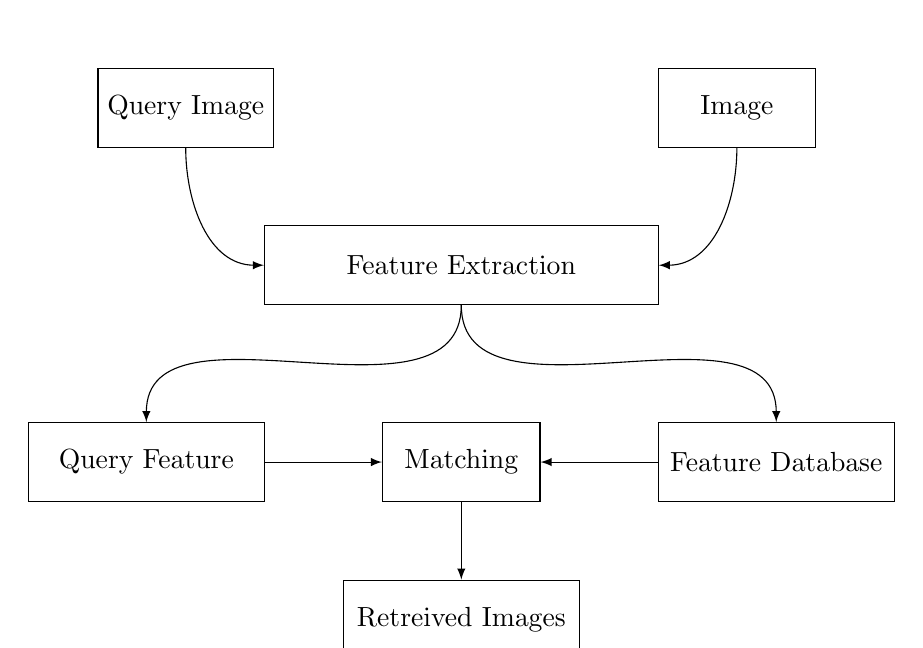
\begin{tikzpicture}[node distance=2cm]
			
			%Nodes	
			\node (queryImage) at (-3.5, 0) [rectangle, draw, text centered, minimum width=2cm, 
			minimum height=1cm] {Query Image};
			
			\node (image) at ( 3.5, 0) [rectangle, text centered, draw, minimum width=2cm, minimum 
			height=1cm] {Image};
			
			\node (featureExtraction) at ( 0,-2) [rectangle, draw, text centered, minimum 
			width=5cm, minimum height=1cm] {Feature Extraction};
			
			\node (queryFeature) at (-4,-4.5) [rectangle, draw, text centered, minimum width=3cm, 
			minimum height=1cm] {Query Feature};
			
			\node (matching) at ( 0,-4.5) [rectangle, draw, text centered, minimum width=2cm, 
			minimum height=1cm] {Matching};
			
			\node (featureDatabase) at ( 4,-4.5) [rectangle, draw, text centered, minimum 
			width=3cm, minimum height=1cm] {Feature Database};
			
			\node (retreivedImages) at ( 0,-6.5) [rectangle, draw, text centered, minimum 
			width=3cm, minimum height=1cm] {Retreived Images};
			
			%Links
			\draw [-latex] (queryFeature.east) -- (matching.west);
			\draw [-latex] (featureDatabase.west) -- (matching.east);
			\draw [-latex] (matching.south) -- (retreivedImages.north);
			\draw [-latex] (queryImage) to [out=270,in=180] (featureExtraction);
			\draw [-latex] (image) to [out=270,in=0] (featureExtraction);
			\draw [-latex] (featureExtraction) to [out=270,in=90] (queryFeature);
			\draw [-latex] (featureExtraction) to [out=270,in=90] (featureDatabase);
			
			\end{tikzpicture}
		}
	\end{center}
\end{figure}

\newpage

\section{Example \theblockDiagram}
\stepcounter{blockDiagram}

\begin{figure}[h]
	\begin{center}
		\scalebox{0.95}{
		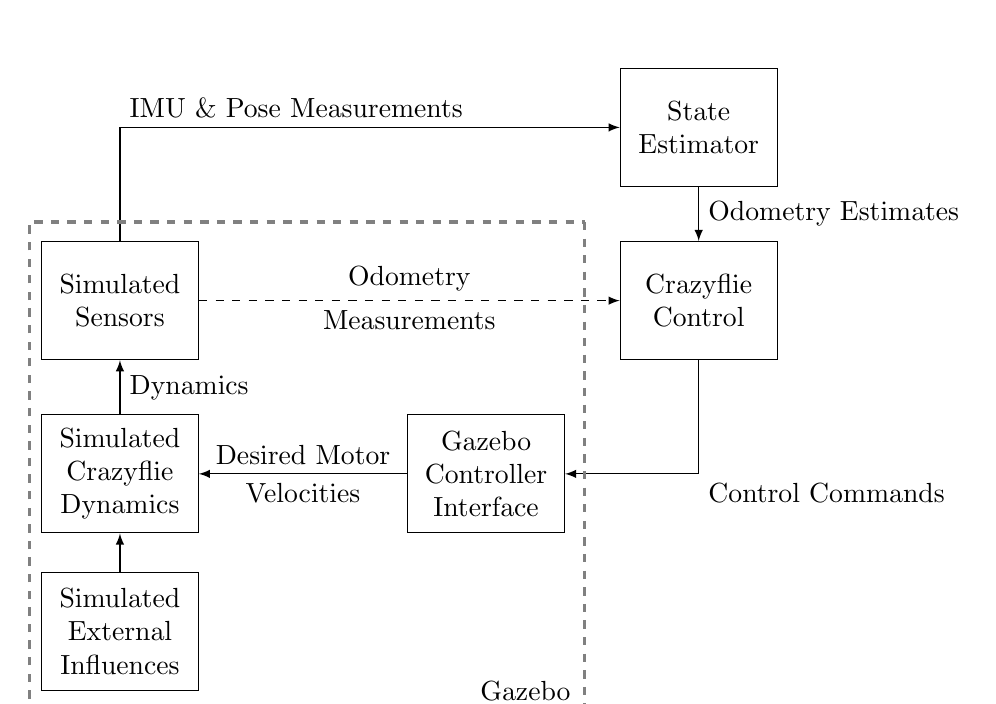
\begin{tikzpicture}
		
		%Blocks
		\node (CrazyflieControl) at (0.2,0) [draw, rectangle, minimum width=1.5cm, minimum 
		height=1.5cm, text centered, text width=5em]{Crazyflie Control};
		\node (GazeboControllerInterface) at (-2.5,-2.2) [draw, rectangle, minimum width=1.5cm, 
		minimum height=1.5cm, text centered, text width=5em]{Gazebo Controller\\Interface};
		\node (SimulatedExternalInfluence) at (-7.15,-4.2) [draw, rectangle, minimum 
		width=1.5cm, minimum height=1.5cm, text centered, text width=5em]{Simulated 
		External\\Influences};
		\node (SimulatedCrazyflieDynamics) at (-7.15,-2.2) [draw, rectangle, minimum 
		width=1.5cm, minimum height=1.5cm, text centered, text width=5em]{Simulated 
		Crazyflie\\Dynamics};
		\node (SimulatedSensor) at (-7.15,0) [draw, rectangle, minimum width=1.5cm, minimum 
		height=1.5cm, text centered, text width=5em]{Simulated Sensors};
		\node (StateEstimator) at (0.2,2.2) [draw, rectangle, minimum width=1.5cm, minimum 
		height=1.5cm, text centered, text width=5em]{State Estimator};
		
		%Links
		\draw[-latex] (CrazyflieControl) |- node[below right]{Control Commands} 
		(GazeboControllerInterface);
		\draw[-latex] (GazeboControllerInterface) -- node[above]{Desired Motor} 
		node[below]{Velocities} (SimulatedCrazyflieDynamics);
		\draw[-latex] (SimulatedExternalInfluence) -- (SimulatedCrazyflieDynamics);
		\draw[-latex] (SimulatedSensor) |- node[above right]{IMU \& Pose Measurements} 
		(StateEstimator);
		\draw[-latex] (StateEstimator) -- node[right]{Odometry Estimates} (CrazyflieControl);
		\draw[-latex] (SimulatedCrazyflieDynamics) -- node[right] {Dynamics} (SimulatedSensor);
		\draw[-latex, dashed] (SimulatedSensor) -- node[above]{Odometry} 
		node[below]{Measurements} (CrazyflieControl) ;
		
		%Gazebo's group
		\draw[dashed, gray, draw, line width=1.25pt] (-1.25,1) coordinate -- (-1.25,-5.25) 
		coordinate -- (-8.3,-5.25) coordinate -- (-8.3,1) coordinate -- (-1.25,1) coordinate; 
		\draw (-2,-5.2) coordinate node[above]{Gazebo};
		
		\end{tikzpicture}
	}
	\end{center}
\end{figure}



\section{Example \theblockDiagram}
\stepcounter{blockDiagram}

\begin{figure}[h]
	\begin{center}
		\scalebox{0.9}{
			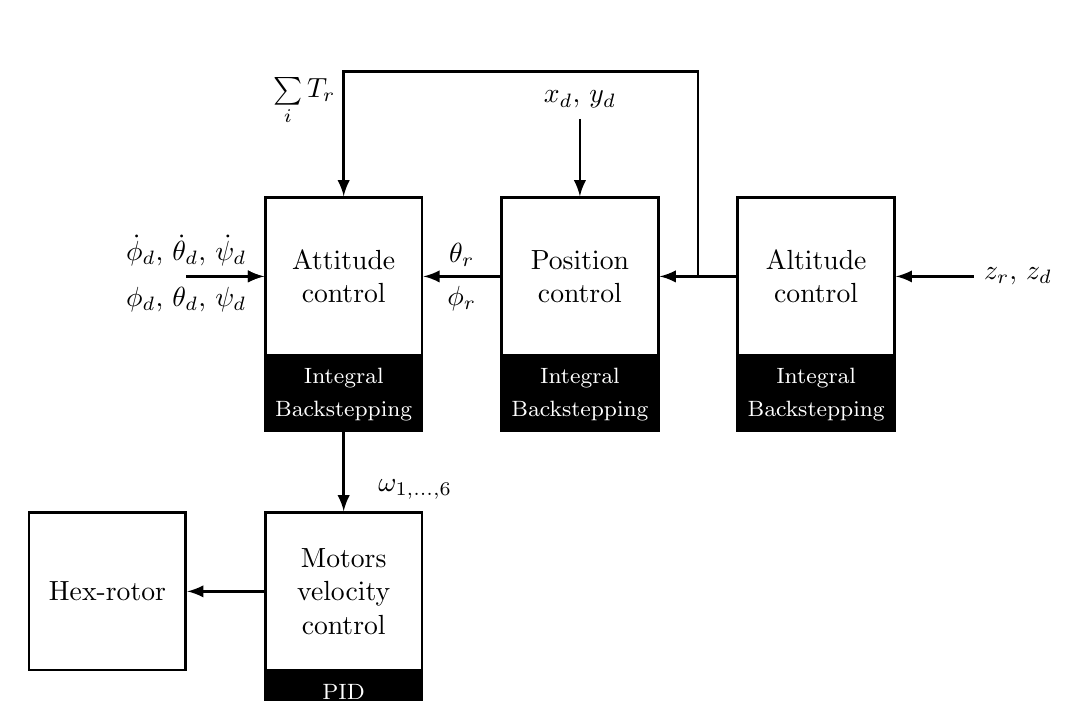
\begin{tikzpicture}
			
			%Attitude controller
			\node (attitudeController) at (-3,0) [draw, rectangle, text centered, line width=1.0pt, 
			minimum height=2cm, minimum width=1cm, text width=5em]{Attitude\\ control};
			
			%baseline Integral Backstepping
			\node (baselineIntegralBackstepping) at (-3,-1.50) [draw, line width=1.0pt, fill=black, 
			rectangle, minimum height=0.5cm, minimum width=1cm, text centered, text 
			width=5em]{\footnotesize{\color{white}{Integral\\ Backstepping}}}; 
			
			%PositionController
			\node (positionController) at (0,0) [draw, rectangle, line width=1.0pt, text centered, 
			minimum height=2cm, minimum width=1cm, text width=5em]{Position\\ control};
			
			%Baseline Integral Backstepping
			\node at (0,-1.50) [draw, line width=1.0pt, fill=black, rectangle, minimum 
			height=0.5cm, minimum width=1cm, text centered, text 
			width=5em]{\footnotesize{\color{white}{Integral\\ Backstepping}}}; 
			
			%Altitude controller
			\node (altitudeController) at (3,0) [draw, rectangle, line width=1.0pt, text centered, 
			minimum height=2cm, minimum width=1cm, text width=5em]{Altitude\\ control};
			
			%Baseline Integral Backstepping
			\node at (3,-1.50) [draw, line width=1.0pt, fill=black, rectangle, minimum 
			height=0.5cm, minimum width=1cm, text centered, text 
			width=5em]{\footnotesize{\color{white}{Integral\\ Backstepping}}}; 
			
			%Motors controller
			\node (motorsController) at (-3,-4) [draw, rectangle, line width=1.0pt, text 
			centered, minimum height=2cm, minimum width=1cm, text width=5em]{Motors velocity 
			control};
			
			%Baseline PID
			\node at (-3,-5.28) [draw, line width=1.0pt, fill=black, rectangle, minimum 
			height=0.5cm, minimum width=1cm, text centered, text 
			width=5em]{\footnotesize{\color{white}{PID}}}; 
			
			%Hexarotor
			\node (hexarotor) at (-6,-4) [draw, rectangle, line width=1.0pt, text centered, 
			minimum height=2cm, minimum width=1cm, text width=5em]{Hex-rotor};
			
			%Links
			\draw[-latex, line width=1.0pt] (motorsController.west) -- (hexarotor.east);
			\draw[-latex, line width=1.0pt] (altitudeController.west) -- (positionController.east);
			\draw[-latex, line width=1.0pt] (positionController.west) -- (attitudeController.east);
			\draw[-latex, line width=1.0pt] (baselineIntegralBackstepping.south) -- 
			(motorsController.north);
			
			\draw[-latex, line width=1.0pt] (1.5,0) coordinate -- (1.5,2.6) coordinate -- (-3,2.6) 
			coordinate -- (attitudeController.north);
			
			%Reference signals
			\draw[-latex, line width=1.0pt] (5,0) coordinate node[right]{$z_r,\,z_d$}-- 
			(altitudeController.east);
			\node[above] at (-3.5,1.8) [text centered]{$\sum\limits_i T_r$};
			\draw[-latex, line width=1.0pt] (0,2) coordinate node[above]{$x_d,\,y_d$} -- 
			(positionController.north);
			\node[above] at (-1.5,0) [text centered]{$\theta_r$};
			\node[below] at (-1.5,0) [text centered]{$\phi_r$};
			\draw[-latex, line width=1.0pt] (-5.0,0) coordinate 
			node[below]{$\phi_d,\,\theta_d,\,\psi_d$} -- (attitudeController.west);
			\draw[-latex, line width=1.0pt] (-5.0,0) coordinate 
			node[above]{$\dot{\phi}_d,\,\dot{\theta}_d,\,\dot{\psi}_d$} -- 
			(attitudeController.west);
			\node at (-1.5,-2.7) [left, text centered]{$\omega_{1,\dots,6}$}; 
			
			\end{tikzpicture}
		}
	\end{center}
	
	
\end{figure}

\newpage




\section{Example \theblockDiagram}
\stepcounter{blockDiagram}

\begin{figure}[h]
	\begin{center}
		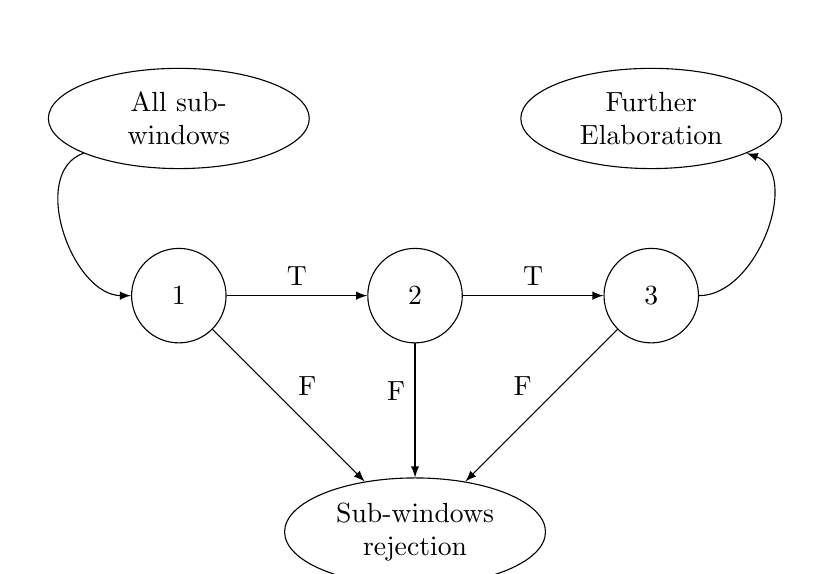
\begin{tikzpicture}[node distance=2cm]
		
		%Creo i nodi del diagramma di flusso		
		\node (allSubWindow) at (-3,1) [ellipse, draw, text centered, text width=6em] {All 
		sub-windows};
		
		\node (furtherProcessing) at (3,1) [ellipse, draw, text centered, text width=6em] {Further 
		Elaboration};
		
		\node (1) at (-3,-1.25) [circle, draw, text centered, minimum size=1.2cm] {1};
		
		\node (2) at (0,-1.25) [circle, draw, text centered, minimum size=1.2cm] {2};
		
		\node (3) at (3,-1.25) [circle, draw, text centered, minimum size=1.2cm] {3};
		
		\node (rejectSubWindows) at (0,-4.25) [ellipse, draw, text centered, text width=6em] 
		{Sub-windows rejection};
		
		\draw[-latex] (1) -- node[above]{T} (2);
		\draw[-latex] (2) -- node[above]{T} (3);
		\draw[-latex] (2) -- node[above left]{F} (rejectSubWindows);
		\draw[-latex] (1) -- node[above right]{F} (rejectSubWindows);
		\draw[-latex] (3) -- node[above left]{F} (rejectSubWindows);
		\draw[-latex] (allSubWindow) to [out=200,in=180] (1);
		\draw[-latex] (3) to [out=0, in=340] (furtherProcessing);
		
		\end{tikzpicture}
	\end{center}
	
\end{figure}

\section{Example \theblockDiagram}
\stepcounter{blockDiagram}

\begin{figure}[h]
	\begin{center}
		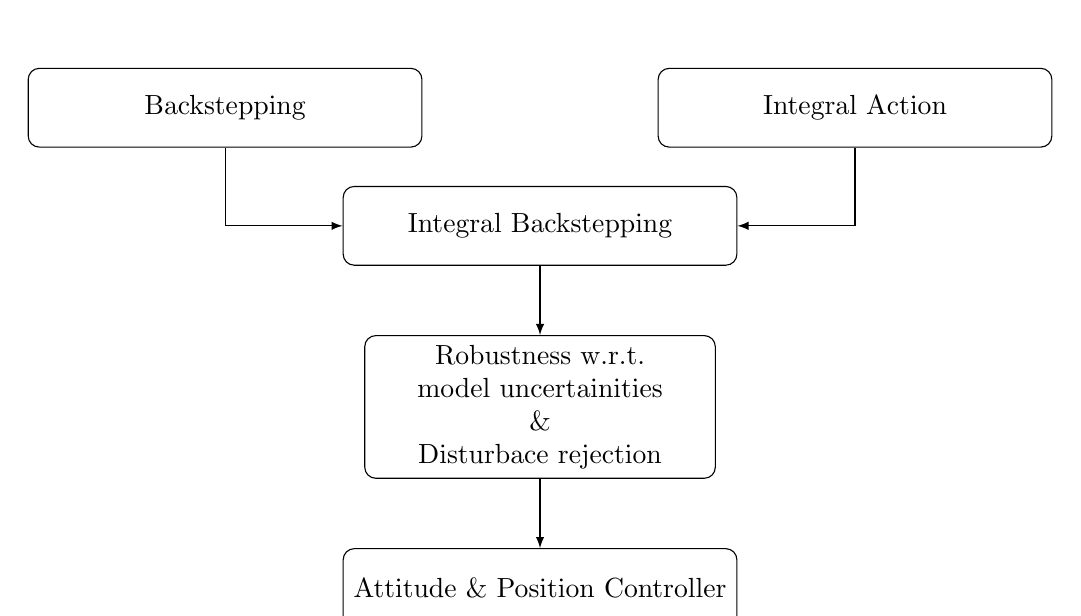
\begin{tikzpicture}
		
		%Nodes
		\node (BackStepping) at (-4,1.5) [draw, rectangle, minimum height=1cm, minimum width=5cm, 
		text centered, rounded corners]{Backstepping};
		\node (integralAction) at (4,1.5) [draw, rectangle, minimum height=1cm, minimum width=5cm, 
		text centered, rounded corners]{Integral Action};
		
		%Rappresento il nodo centrale
		\node (integralBackStepping) at (0,0) [draw, rectangle, minimum height=1cm, minimum 
		width=5cm, text centered, rounded corners]{Integral Backstepping};
		
		%Rappresento il blocco caratteristiche
		\node (features) at (0,-2.3) [draw, rectangle, minimum height=1cm, minimum 
		width=1cm, text centered, rounded corners, text width=12em]{Robustness w.r.t. model 
		uncertainities\\ \& \\Disturbace rejection};
		
		%Control system results
		\node (results) at (0,-4.6) [draw, rectangle, minimum height=1cm, minimum width=5cm, text 
		centered, rounded corners]{Attitude \& Position Controller};
		
		%Links
		\draw[-latex] (BackStepping.270) -- (-4,0) coordinate -- (integralBackStepping.180);
		\draw[-latex] (integralAction.270) -- (4,0) coordinate -- (integralBackStepping.0);
		\draw[-latex] (integralBackStepping.south) -- (features.north);
		\draw[-latex] (features.south) -- (results.north);
		
		
		\end{tikzpicture}
	\end{center}
	
\end{figure}

\newpage


\section{Example \theblockDiagram}
\stepcounter{blockDiagram}

\begin{figure}[h]
	\begin{center}
		\scalebox{0.8}{
		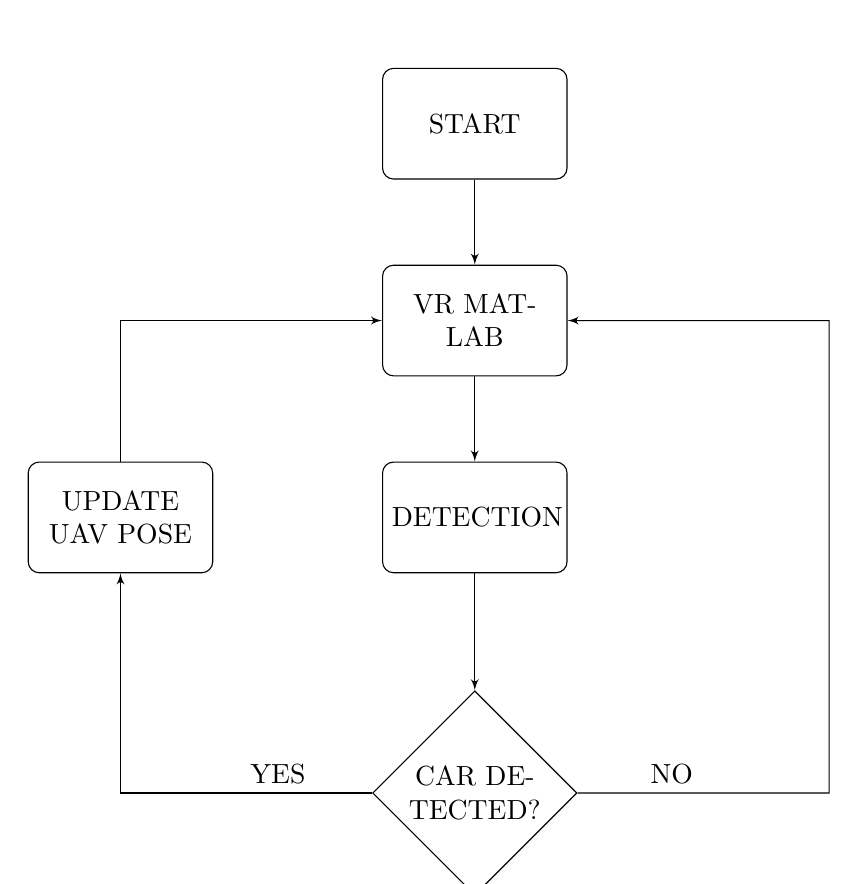
\begin{tikzpicture}
		
		%System nodes
		\node [rectangle, draw, text width=6em, text centered, rounded corners, minimum height=4em] 
		(start) at (0,0) {START};
		
		\node [rectangle, draw, text width=6em, text centered, rounded corners, minimum height=4em, 
		below of=init] (vrMatlab) at (0,-1.5) {VR MATLAB};
		
		\node [rectangle, draw, text width=6em, text centered, rounded corners, minimum height=4em, 
		below of=identify] (detection) at (0,-4.0) {DETECTION};
		
		\node [rectangle, draw, text width=6em, text centered, rounded corners, minimum height=4em, 
		left of=evaluate, node distance=3cm] (update) at (-1.5,-5) {UPDATE UAV POSE};
		
		\node [diamond, draw, text width=5.5em, text badly centered, node distance=3cm, inner 
		sep=0pt, below of=evaluate] (decide) at (0,-5.5) {CAR DETECTED?};
		
		
		%Links
		\path [draw, -latex'] (start) -- (vrMatlab);
		\path [draw, -latex'] (vrMatlab) -- (detection);
		\path [draw, -latex'] (detection) -- (decide);
		\path [draw, -latex'] (decide) -| (update);
		\path [draw, -latex'] (update) |- (vrMatlab);
		\path [draw, -latex'] (decide.east) -- (4.5,-8.5) coordinate -- (4.5,-2.5) coordinate -- 
		(vrMatlab.east);
		
		%Decisions
		\node at (2.5,-8.5)  [above] {NO};
		\node at (-2.5,-8.5) [above] {YES};
		
		\end{tikzpicture}
	}
	\end{center}
	
\end{figure}

\newpage

\section{Example \theblockDiagram}
\stepcounter{blockDiagram}

\begin{figure}[h]
	\begin{center}
		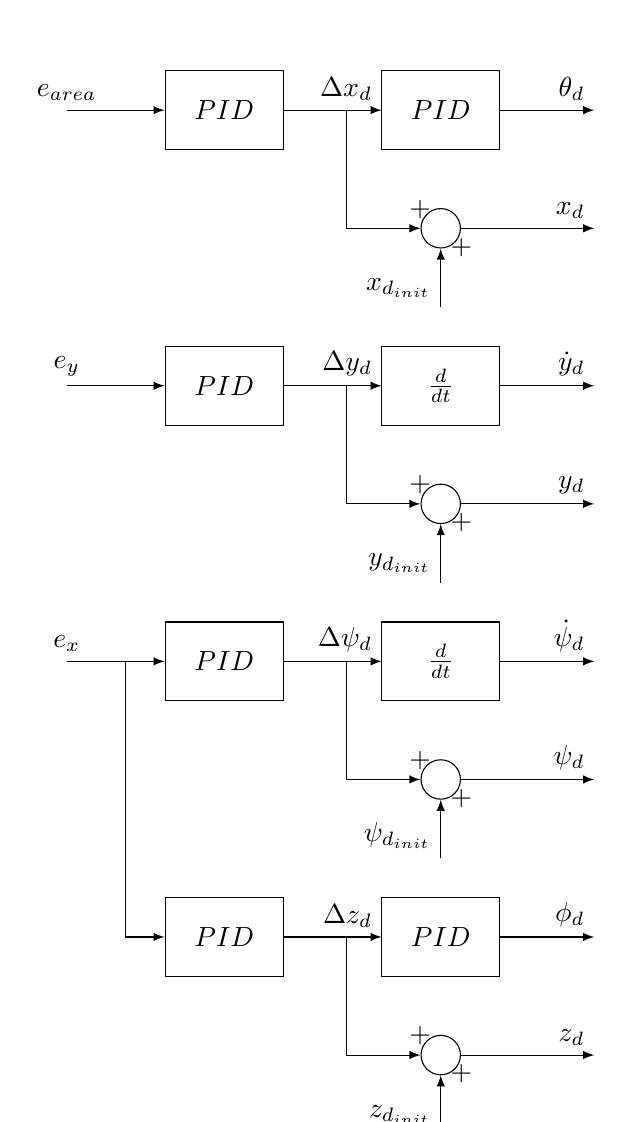
\begin{tikzpicture}
		
		%Nodes
		\node (firstPID) at (-2,0.5) [draw, rectangle, minimum width=1.5cm, minimum height=1cm, 
		text centered]{$PID$};
		
		\node (secondPID) at (0.75,0.5) [draw, text centered, minimum width=1.5cm, minimum 
		height=1cm]{$PID$};
		
		\node (adder) at (0.75,-1) [draw, circle, text centered, minimum size=0.5cm]{};
		
		%Links
		\draw[-latex] (-4,0.5) coordinate node[above]{$e_{area}$} -- (firstPID.west);
		
		\draw[-latex] (firstPID.east) -- (0,0.5) coordinate node[above left]{$\Delta x_d$};
		
		\draw[-latex] (secondPID.east) -- (2.7,0.5) coordinate node[above left]{$\theta_d$};
		
		\draw[-latex] (-0.45,0.5) coordinate -- (-0.45,-1) coordinate -- (adder.west);
		
		\draw[-latex] (adder.east) -- (2.7,-1) coordinate node[above left]{$x_d$};
		
		\draw[-latex] (0.75,-2.0) coordinate node[above left]{$x_{d_{init}}$} -- (adder.south);
		
		%Signs
		\draw (0.75,-1) coordinate node[above left]{$+$};
		\draw (0.75,-1) coordinate node[below right]{$+$};
		
		%Names into the second part of the scheme
		\node (thirdPID) at (-2,-3.0) [draw, rectangle, minimum width=1.5cm, minimum height=1cm, 
		text centered]{$PID$};
		
		\node (fourthPID) at (0.75,-3.0) [draw, text centered, minimum width=1.5cm, minimum 
		height=1cm]{$\frac{d}{dt}$};
		
		\node (adder1) at (0.75,-4.5) [draw, circle, text centered, minimum size=0.5cm]{};
		
		%Links among blocks
		\draw[-latex] (-4,-3.0) coordinate node[above]{$e_y$} -- (thirdPID.west);
		
		\draw[-latex] (thirdPID.east) -- (0,-3.0) coordinate node[above left]{$\Delta y_d$};
		
		\draw[-latex] (fourthPID.east) -- (2.7,-3.0) coordinate node[above left]{$\dot{y}_d$};
		
		\draw[-latex] (-0.45,-3.0) coordinate -- (-0.45,-4.5) coordinate -- (adder1.west);
		
		\draw[-latex] (adder1.east) -- (2.7,-4.5) coordinate node[above left]{$y_d$};
		
		\draw[-latex] (0.75,-5.5) coordinate node[above left]{$y_{d_{init}}$} -- (adder1.south);
		
		%Signs
		\draw (0.75,-4.5) coordinate node[above left]{$+$};
		\draw (0.75,-4.5) coordinate node[below right]{$+$};
		
		%Third part of the scheme
		\node (fifthPID) at (-2,-6.5) [draw, rectangle, minimum width=1.5cm, minimum height=1cm, 
		text centered]{$PID$};
		
		\node (sixthPID) at (0.75,-6.5) [draw, text centered, minimum width=1.5cm, minimum 
		height=1cm]{$\frac{d}{dt}$};
		
		\node (adder2) at (0.75,-8.0) [draw, circle, text centered, minimum size=0.5cm]{};
		
		%Links among blocks
		\draw[-latex] (-4,-6.5) coordinate node[above]{$e_x$} -- (fifthPID.west);
		
		\draw[-latex] (fifthPID.east) -- (0,-6.5) coordinate node[above left]{$\Delta \psi_d$};
		
		\draw[-latex] (sixthPID.east) -- (2.7,-6.5) coordinate node[above left]{$\dot{\psi}_d$};
		
		\draw[-latex] (-0.45,-6.5) coordinate -- (-0.45,-8.0) coordinate -- (adder2.west);
		
		\draw[-latex] (adder2.east) -- (2.7,-8.0) coordinate node[above left]{$\psi_d$};
		
		\draw[-latex] (0.75,-9.0) coordinate node[above left]{$\psi_{d_{init}}$} -- 
		(adder2.south);
		
		%Signs
		\draw (0.75,-8.0) coordinate node[above left]{$+$};
		\draw (0.75,-8.0) coordinate node[below right]{$+$};
		
		
		%Signs
		\node (seventhPID) at (-2,-10) [draw, rectangle, minimum width=1.5cm, minimum height=1cm, 
		text centered]{$PID$};
		
		\node (eighthPID) at (0.75,-10) [draw, text centered, minimum width=1.5cm, minimum 
		height=1cm]{$PID$};
		
		\node (adder3) at (0.75,-11.5) [draw, circle, text centered, minimum size=0.5cm]{};
		
		%Links
		\draw[-latex] (-3.25,-6.5) coordinate -- (-3.25,-10) coordinate -- (seventhPID.west);
		
		\draw[-latex] (seventhPID.east) -- (0,-10) coordinate node[above left]{$\Delta z_d$};
		
		\draw[-latex] (eighthPID.east) -- (2.7,-10) coordinate node[above left]{$\phi_d$};
		
		\draw[-latex] (-0.45,-10) coordinate -- (-0.45,-11.5) coordinate -- (adder3.west);
		
		\draw[-latex] (adder3.east) -- (2.7,-11.5) coordinate node[above left]{$z_d$};
		
		\draw[-latex] (0.75,-12.5) coordinate node[above left]{$z_{d_{init}}$} -- (adder3.south);
		
		%Signs
		\draw (0.75,-11.5) coordinate node[above left]{$+$};
		\draw (0.75,-11.5) coordinate node[below right]{$+$};
		\end{tikzpicture}
	\end{center}
	
\end{figure}
\chapter{Matlab Plots}
\label{chapter:matlabPlots}


\newcounter{matlabPlots}
\setcounter{matlabPlots}{0}
\stepcounter{matlabPlots}

%%%%%%%%%%%%%%%%%%%%%%%%%%%%%%%%%%%%%%%%%%%%%%%%%%%%%%%%%%%%%%%%%%%%%%%%%%%%%%%%%%%%%%%%%%%%%%%%%%%%

\section{Example \thematlabPlots}
\stepcounter{matlabPlots}

\begin{figure}[h]
	\begin{center}
		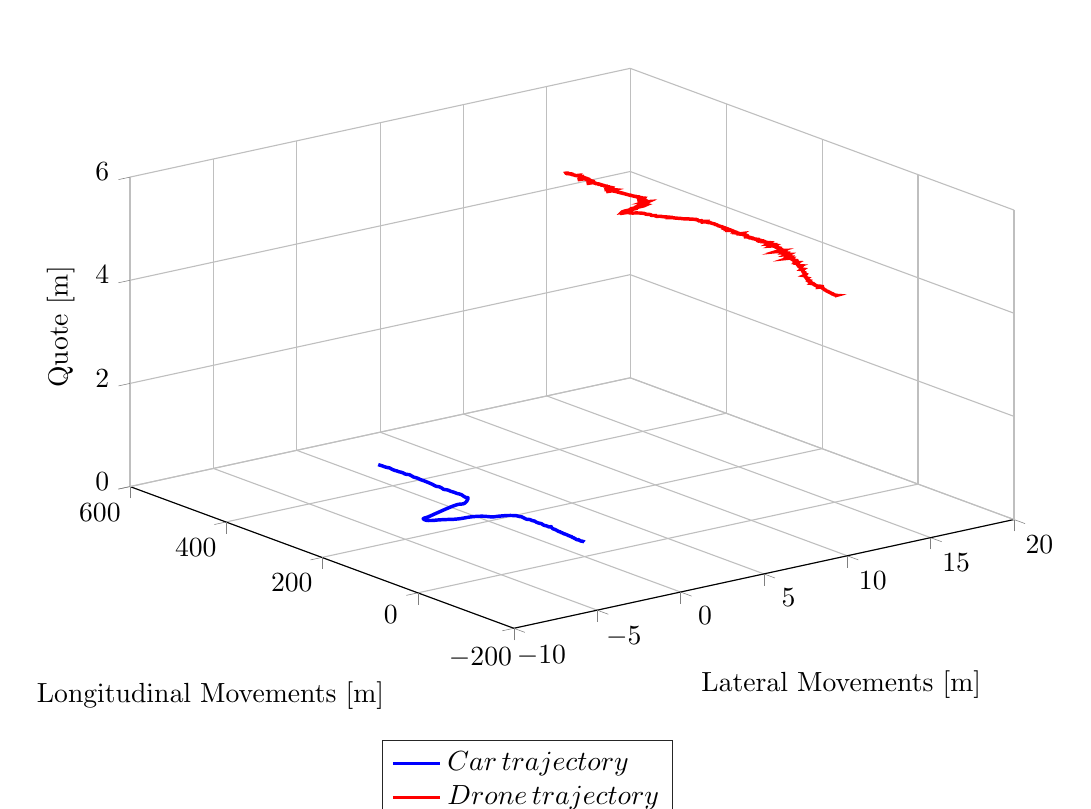
\begin{tikzpicture}
		
		\begin{axis}[
		width=4.42in,
		height=2.80in,
		at={(0.508in,0.481in)},
		scale only axis,
		xmin=-10,
		xmax=20,
		tick align=outside,
		xlabel={Lateral Movements~[\si{\meter}]},
		xmajorgrids,
		ymin=-200,
		ymax=600,
		ylabel={Longitudinal Movements~[\si{\meter}]},
		ymajorgrids,
		zmin=0,
		zmax=6,
		zlabel={Quote~[\si{\meter}]},
		zmajorgrids,
		view={-37.5}{30},
		axis x line*=bottom,
		axis y line*=left,
		axis z line*=left,
		legend style={at={(0.45,-0.20)},anchor=north,legend cell align=left,align=left,draw=white!15!black}
		]
		\addplot3 [color=blue,solid, line width=1.25pt]
		table[row sep=crcr] {%
			0.00112327469008465	0.414227033373808	0.280461005424321\\
			0.00117633264854411	0.451421155639095	0.280646600151087\\
			0.00119630200319756	0.490178859768547	0.280857519528042\\
			0.00103004090059024	0.572379482203284	0.281347000757606\\
			0.000779831459974425	0.61583615727973	0.281613590881281\\
			0.000479940268713286	0.66087648334289	0.281890931510847\\
			0.000155281239941537	0.707505335803026	0.28217964025511\\
			-0.000396667638717687	0.805512054366473	0.282773861857388\\
			-0.000599522091734537	0.856860794009249	0.283058565049005\\
			-0.000769314750710044	0.909752739752476	0.283321379395942\\
			-0.000936069033441722	0.964160123431321	0.283545400868146\\
			-0.00136491823484834	1.07742578552504	0.283767337964615\\
			-0.00163508227646295	1.13628926428492	0.283796358830326\\
			-0.00193033367488557	1.19665172885688	0.283799903078144\\
			-0.0022492101139531	1.25851034370219	0.283785447551125\\
			-0.00292195825149391	1.38675578558442	0.283894346368599\\
			-0.0032244860599107	1.45315283186511	0.284063154858169\\
			-0.00347320181554705	1.5210700229887	0.28430156532987\\
			-0.00365353554960231	1.59052278015791	0.284590730583846\\
			-0.00389480290134993	1.73404076220728	0.285039666259844\\
			-0.00405340370328729	1.8081098227614	0.285160861524737\\
			-0.004286158042384	1.88371189091593	0.285222603244192\\
			-0.00460404123823578	1.96084884715931	0.285273652457125\\
			-0.00538911066968552	2.11975290634612	0.285442766060552\\
			-0.00580734994083134	2.20152915988469	0.285533862159143\\
			-0.00621381478137001	2.28486032870633	0.285589024237041\\
			-0.00660127997145246	2.36973437867582	0.285558940550944\\
			-0.00734738908019772	2.54411392450883	0.285288592011988\\
			-0.00774941470227535	2.63359944133627	0.285070772206548\\
			-0.00816515462748415	2.72459662552308	0.284839170759315\\
			-0.0085398152634138	2.81709677950506	0.284628286244952\\
			-0.00893001504671477	3.00657971704751	0.28433627283415\\
			-0.00895219464751484	3.1035600234596	0.284268493647583\\
			-0.00894931412459765	3.20202096385955	0.284238004857139\\
			-0.0089917799653094	3.30195434704088	0.284233575332782\\
			-0.00931469779737402	3.50626480298683	0.284295283129175\\
			-0.00959916564301333	3.6106874077523	0.284326147226178\\
			-0.00997810846320024	3.7166376565894	0.284327695513193\\
			-0.0104242084333782	3.8240960797903	0.284313419550395\\
			-0.0113472658654939	4.04349064798117	0.284495995357708\\
			-0.0117866927733141	4.15544241390233	0.284676506937316\\
			-0.0122256693644301	4.26890997506648	0.284785424782461\\
			-0.012648723460717	4.38387852723946	0.28475384365241\\
			-0.013236429935056	4.61826951395467	0.28455665379104\\
			-0.0133663692249308	4.73772479042464	0.284516477757302\\
			-0.0134622306303687	4.85872888442964	0.284444193794836\\
			-0.0135971761862901	4.98127619334415	0.284227632537487\\
			-0.0140474289995148	5.23097467085517	0.283573778912742\\
			-0.0143316208239754	5.35811718482281	0.28330052187255\\
			-0.0146038413882078	5.48678598008737	0.283029073295505\\
			-0.0148307818305098	5.6169575039224	0.282638209391609\\
			-0.015020968063603	5.88182528495016	0.281502536976326\\
			-0.0149213808374881	6.0165480278282	0.280842594079139\\
			-0.0146480120410801	6.15282137640777	0.280163676534813\\
			-0.0142184838881663	6.2906681950887	0.27952007145884\\
			-0.0133200724692108	6.57100170562415	0.278546038804183\\
			-0.0130499241218501	6.71345321866003	0.2782204425919\\
			-0.0130069759840851	6.8574500445939	0.278012541901416\\
			-0.0131534756679507	7.00299928836965	0.277928730855072\\
			-0.0134012197126943	7.29864837736615	0.278017766027808\\
			-0.0134148894399678	7.44875721200382	0.278036169551846\\
			-0.0134070862302746	7.60039854456227	0.277919029691224\\
			-0.0133481939974801	7.75355569781088	0.277771687838998\\
			-0.0130884575886097	8.06441012264432	0.277696748158765\\
			-0.013052816347077	8.22212492980168	0.277738039007037\\
			-0.0130326118308583	8.38138532404036	0.277911038832203\\
			-0.0129127072675147	8.54218697814418	0.278266516916572\\
			-0.0121255451476853	8.86842689279965	0.279319765830652\\
			-0.0116372337620332	9.03383812487689	0.279997749405166\\
			-0.0113412052310816	9.20076770065879	0.280714823138494\\
			-0.0113460641781888	9.36915881125476	0.281139927050491\\
			-0.0119932935988385	9.71027324962687	0.280928288776868\\
			-0.01232231504591	9.88304397463228	0.280683298584269\\
			-0.0125206829995466	10.0573544331669	0.280653081233573\\
			-0.0125765428650953	10.2331995235417	0.280872396767314\\
			-0.012297054407168	10.5894303235186	0.282009161577924\\
			-0.0120406351851977	10.7697754065403	0.282547232168821\\
			-0.0117960731557997	10.9515827850586	0.283035586251695\\
			-0.0115677373006213	11.1348555974983	0.283560852487683\\
			-0.0110632450420035	11.5057514873614	0.284347637924\\
			-0.0108964812672247	11.6933493557221	0.284773701970858\\
			-0.0107904921964239	11.8824503123089	0.285316789129178\\
			-0.0106616407734817	12.0731445032621	0.285827610659002\\
			-0.0104200378255119	12.4589713436929	0.285535256550229\\
			-0.0102081789997352	12.653991554136	0.284780751554944\\
			-0.00987535360898057	12.8504275443947	0.283824079827945\\
			-0.0094159336233861	13.0483225158976	0.282763711043706\\
			-0.00823379132955148	13.4487225643104	0.280796105854331\\
			-0.00767748723863528	13.6512381735167	0.27991664531075\\
			-0.007190803891867	13.8552909893843	0.279071089646803\\
			-0.00678962017381392	14.0608857802985	0.278276233587234\\
			-0.00635685101890209	14.4765665816365	0.277013701092341\\
			-0.006181901182403	14.6867435476359	0.276597705304252\\
			-0.0061185192010231	14.8985112215799	0.276151337106818\\
			-0.00612246811678515	15.1118659080065	0.27568145773278\\
			-0.00566467524677815	15.5432717069713	0.274965661951942\\
			-0.00511398642631606	15.7612799207756	0.274672875072325\\
			-0.00443300780206835	15.9808205444687	0.274379354059374\\
			-0.00372777624797551	16.2019160348685	0.274234688487701\\
			-0.00260529456384661	16.6487539459775	0.27408635836642\\
			-0.00238756906071181	16.8743989256052	0.274019858850571\\
			-0.00224548537674224	17.1015551476014	0.274120798586486\\
			-0.00210256583889857	17.3302629526204	0.274520058951983\\
			-0.00182938306858292	17.7923461398106	0.275882581723673\\
			-0.00163637415557382	18.0256016931774	0.27655990942562\\
			-0.0013215587725846	18.2603552330804	0.2772715745075\\
			-0.000775278794568724	18.4966070651673	0.277795241149602\\
			0.000286406152431358	18.9735203364745	0.278641666316669\\
			0.000587916382624959	19.2141403503842	0.278920615991036\\
			0.000819902152367811	19.4562488614352	0.27920752757089\\
			0.00112470885326643	19.6998079620333	0.279551131671765\\
			0.00196286692282594	20.1913120717111	0.280549858669905\\
			0.00232743506435695	20.43934925314	0.281218863183503\\
			0.00247491025685823	20.6888383118224	0.281750585779161\\
			0.00262064768202632	20.9397899758198	0.281878364256866\\
			0.00297938887034238	21.4461486447474	0.282032455387715\\
			0.00314460235561193	21.701579393169	0.282304736114641\\
			0.00328819852838727	21.9584576125541	0.282583503526949\\
			0.00348795478231339	22.2168039206639	0.282947094059922\\
			0.00422751676082328	22.7380262112989	0.284267544195017\\
			0.00457720971648446	23.0008104518527	0.284627427666512\\
			0.00472769196204589	23.2651437471299	0.285001184692387\\
			0.00477245667310052	23.5310463640148	0.285220977584655\\
			0.00457100697028544	24.0670999892185	0.284400655344042\\
			0.00445174026386549	24.3372646334843	0.283902689768965\\
			0.00437314041235549	24.6088956977887	0.283444830864576\\
			0.00448352034701243	24.8819916563291	0.283163553424151\\
			0.00541375564492816	25.43272083035	0.283341801062937\\
			0.00586429729369597	25.7103772202831	0.283796592221974\\
			0.00638789410227818	25.9895896758753	0.28468549816589\\
			0.00695847562271911	26.2703724593305	0.285903819249675\\
			0.00777645073384103	26.8365613887856	0.289198738894624\\
			0.00798030460042814	27.1217308072137	0.290445391859269\\
			0.00817511138739492	27.4083110921703	0.291274537503758\\
			0.00835725748298789	27.6962600939711	0.291702397595181\\
			0.0087294097823708	28.2763446867979	0.29157181601794\\
			0.00913876152479926	28.5685155167445	0.291227145882671\\
			0.00976762142906529	28.862133072822	0.290787487259847\\
			0.0104102724828365	29.157198309273	0.290391107936633\\
			0.0113122005987191	29.7518545455938	0.290057112227562\\
			0.0117710234754622	30.0515775821505	0.290149422594796\\
			0.0120992366513816	30.3527725237625	0.290167350936163\\
			0.0123626998906676	30.6554677406909	0.290252130594336\\
			0.0131231350929886	31.2653483679823	0.290302119459873\\
			0.0137072501850211	31.5725130836413	0.290212392466685\\
			0.0142368641352486	31.8811318217519	0.290167006257976\\
			0.0146638324105012	32.1911649094299	0.290032964541109\\
			0.0156784329891917	32.8157429736352	0.289675380405977\\
			0.0160121551031184	33.1301695994595	0.288965131828743\\
			0.0164542173693674	33.4460961654899	0.288136308252891\\
			0.017125482916412	33.7635851058267	0.287603494680124\\
			0.0185967183603746	34.4031012426297	0.287263873085837\\
			0.0191687847653927	34.7251048850518	0.28743856882974\\
			0.0197737952168628	35.0486632089624	0.287984166122445\\
			0.0203633757464827	35.3737630552632	0.288775754723543\\
			0.0214470479163452	36.028676481988	0.290367536073937\\
			0.0219797054216384	36.3583266051762	0.291004655609212\\
			0.0223473831813745	36.6893808259085	0.291500590304018\\
			0.0225658842579468	37.0218462964799	0.291785547495701\\
			0.0231696727065659	37.6910791747478	0.291700441739597\\
			0.0235244809646808	38.0278915956719	0.291721538230249\\
			0.0239658330403725	38.366240006841	0.291907358097166\\
			0.0243939034740709	38.7060848316174	0.292116147248078\\
			0.0249578078043662	39.3901895252815	0.292455725981164\\
			0.0252412367652732	39.7344520641463	0.292296050469103\\
			0.0255600083744358	40.0802171196608	0.292131253156591\\
			0.0258655175378237	40.4274070630388	0.29195647954054\\
			0.0268502804377305	41.1261607944154	0.291863102498287\\
			0.0273801636845394	41.4777541741011	0.29202687129168\\
			0.0279243373554302	41.8308584757017	0.292065454225804\\
			0.0285592486491912	42.185473419172	0.291787595510102\\
			0.0295981381358146	42.8990515954282	0.290635985511199\\
			0.0301338538654767	43.2579867889352	0.289836853100012\\
			0.0307760574391854	43.6183859700038	0.28915369303081\\
			0.0315114845382912	43.9802871902735	0.288695770652669\\
			0.0330177667751005	44.7086721382226	0.288782837487931\\
			0.0338773979942704	45.0752859475026	0.289623571200549\\
			0.0346195485329634	45.4433865395772	0.290607290555373\\
			0.0352931602981619	45.812918981744	0.291431218946685\\
			0.0368186652880993	46.5562611993647	0.292402474329348\\
			0.0375640574531424	46.9300171873673	0.29247614379727\\
			0.0383182913403033	47.3051435129548	0.292462911583069\\
			0.0391794619659106	47.6816839490979	0.292459069963257\\
			0.0407592756272014	48.439288010354	0.292539210700996\\
			0.0416061313657394	48.8202873589634	0.291952361584369\\
			0.0425327067758002	49.2028363352959	0.291241257125562\\
			0.0434338729638188	49.586870948612	0.290537598999893\\
			0.0451283067981926	50.3594797896966	0.290361570222403\\
			0.0458442670771499	50.7479942626497	0.29051245173927\\
			0.0464309704342324	51.1380804856125	0.29079284550209\\
			0.0470012860323893	51.5298463204819	0.291697940473731\\
			0.0480356168655501	52.3177689162884	0.293966693689652\\
			0.0484890029786972	52.7138112325644	0.295141002921205\\
			0.0488231314211502	53.1111449232666	0.295662733138189\\
			0.049033555070081	53.5098944391385	0.295575121283216\\
			0.0497953050153669	54.3114930403209	0.294295584811726\\
			0.0503186570723343	54.7143744538773	0.293455470953365\\
			0.0509808920432349	55.1187003999388	0.292576127761174\\
			0.0517984686233196	55.5245911361068	0.2920091480259\\
			0.0537818719729313	56.3412232904325	0.29166202941024\\
			0.0547749555866354	56.7517633897818	0.291533818517868\\
			0.0557035041167159	57.1637864551363	0.291769226117755\\
			0.0566566263817	57.5773157563703	0.292431512051487\\
			0.0587395764780218	58.4087978909007	0.294911036679574\\
			0.0597374442834293	58.826659362057	0.295817515019102\\
			0.0605468033006096	59.246069793221	0.297065393006947\\
			0.061298290975875	59.66687797283	0.298195357666076\\
			0.0627482733681055	60.5123604290646	0.298725959049758\\
			0.0636275907387528	60.9373062465286	0.299134725968879\\
			0.0644831725570676	61.3636965042855	0.299268972247756\\
			0.0652383887790245	61.7914766508942	0.299203547118398\\
			0.0669699486576601	62.6514605662468	0.298743827393635\\
			0.0679054846667598	63.0837649491027	0.298902615006951\\
			0.068880932943467	63.5174245094885	0.299030904446174\\
			0.0697724729299537	63.9525237376597	0.299270145995842\\
			0.0716883487811678	64.8272515815735	0.300027642291301\\
			0.0726908018644923	65.2667535512591	0.300131709239964\\
			0.0737147814648756	65.7075853283067	0.299773179335454\\
			0.0747205844178685	66.1498859553238	0.299493194734397\\
			0.0766244020296237	67.0388384532244	0.299190862922798\\
			0.0775832609641198	67.4855019574155	0.298626043652725\\
			0.0785111723578792	67.9336911526099	0.298082284626382\\
			0.0794822998425154	68.3834062296215	0.297722225985188\\
			0.0815272154367905	69.28729386654	0.298206715206162\\
			0.0830439462835533	69.7426186502605	0.2994010022387\\
			0.0849636635474751	70.200446681085	0.300852127949569\\
			0.0873362594865364	70.6612414059508	0.302411244643581\\
			0.0942562102674271	71.5933599537302	0.305684251467154\\
			0.0989590315915926	72.0655585951535	0.307683235856738\\
			0.104674599983944	72.5422456127287	0.309854493451881\\
			0.111479180044585	73.023642068611	0.312069925525267\\
			0.12751671310183	73.9995438522471	0.314697438394057\\
			0.134194262871293	74.4916093274683	0.314403507942675\\
			0.139201907527179	74.9854171772211	0.312811167342916\\
			0.143025690985121	75.4812916367508	0.31051289233482\\
			0.147811538201373	76.4789056681411	0.304399573338963\\
			0.14932390595048	76.9806057567043	0.301256113357357\\
			0.150416791529992	77.4841609367645	0.298467193157226\\
			0.151077627014884	77.989599817504	0.296266655862705\\
			0.151140091739277	79.0061086553663	0.293248348200784\\
			0.150461298610136	79.5171036541354	0.292692917298682\\
			0.149400752643541	80.0298324368865	0.29282003746073\\
			0.147953307048643	80.5442038322499	0.293382671031307\\
			0.144201489584904	81.5779501797448	0.29517795413692\\
			0.141988750411456	82.0970607230955	0.295606320105322\\
			0.139743931051917	82.617661377656	0.296052009343498\\
			0.13754146049938	83.1398168319507	0.296879788028964\\
			0.133249430540487	84.1884210058904	0.297708964685774\\
			0.13128268522224	84.7149797750095	0.297912322550837\\
			0.12953302133421	85.2428780819065	0.297558282416024\\
			0.1280065305869	85.7721040968989	0.296868795310212\\
			0.125693536719218	86.834823823294	0.294898483281432\\
			0.124935683867899	87.3683942107622	0.29416548553592\\
			0.124459165850783	87.9035196614869	0.294001070094024\\
			0.12423704927247	88.440142003414	0.294097069421301\\
			0.124283697297617	89.5177686401655	0.294954058006479\\
			0.124481508316921	90.0585991762844	0.29536028683872\\
			0.124830816009325	90.6008537400201	0.296312569936759\\
			0.125368818438971	91.1445275646876	0.297415274473838\\
			0.126686694794744	92.2361913605133	0.299867821591546\\
			0.127318874920976	92.7840947400256	0.300857631065639\\
			0.128033780368789	93.3333548186673	0.301869837057607\\
			0.128923729636384	93.8840473181688	0.302887556750986\\
			0.130809157128916	94.9894453035973	0.303550396161767\\
			0.131774257046329	95.5442716237734	0.303474143828013\\
			0.132847165381468	96.100429419548	0.302832746529441\\
			0.133933776294819	96.6578701017523	0.301540722894193\\
			0.136249840434346	97.7773249024869	0.299160385551341\\
			0.137510143396607	98.3391656530678	0.2975129420194\\
			0.138809610288352	98.9025803455298	0.296155664183263\\
			0.140105488877555	99.4675520101881	0.295383682792865\\
			0.142751339626631	100.601977620699	0.29500316397868\\
			0.143971725864903	101.17132456386	0.29410953957408\\
			0.145088266911639	101.742068070652	0.293249804873473\\
			0.14616966107681	102.314230074901	0.293026441835929\\
			0.148140248306757	103.463005459257	0.293012524464695\\
			0.148952503389117	104.03974129168	0.29326505744835\\
			0.149722315439725	104.617803309875	0.293337821077528\\
			0.150498710163169	105.197140584435	0.293293814180468\\
			0.152291750393619	106.360298744986	0.294404635432168\\
			0.1532264297693	106.944018951908	0.29516313902674\\
			0.154212131581528	107.529204452197	0.296224357070255\\
			0.155221275864119	108.115837440471	0.297505161477104\\
			0.157120499278757	109.292994991901	0.299829197591321\\
			0.158096504398723	109.88363120135	0.300603807503297\\
			0.159008858759518	110.475495991177	0.300223751535266\\
			0.159854553141014	111.068680556416	0.299162774715468\\
			0.161736376361608	112.25937509313	0.296763095919603\\
			0.16275927362763	112.857029009417	0.295555313219638\\
			0.163768106558505	113.456212633036	0.294241992938036\\
			0.164805261287747	114.056912852566	0.293161663110264\\
			0.16686186513162	115.262496033384	0.291957329594746\\
			0.16781073134141	115.867484806276	0.291673571784735\\
			0.168709308364317	116.47389595298	0.291652359667225\\
			0.169584173021197	117.081732088412	0.292000006632223\\
			0.171231720885501	118.301669764609	0.293241610254922\\
			0.171962921384631	118.913699082939	0.293470691342846\\
			0.172640384113372	119.527039012373	0.29301947544683\\
			0.173353918762169	120.141759351795	0.292411702091676\\
			0.174824901591633	121.375386606071	0.290474986470987\\
			0.175565292153952	121.994398169277	0.288745623725565\\
			0.176336077905533	122.61486160613	0.287017965286987\\
			0.177110395075727	123.236699361377	0.284949453127389\\
			0.178681834728118	124.484680647566	0.279938763070815\\
			0.179533544075973	125.110934865554	0.278061565203264\\
			0.180344115269439	125.738764316136	0.277064118761457\\
			0.181128889992904	126.368143850047	0.276591510987227\\
			0.182380404314103	127.630933186736	0.275174321893879\\
			0.182984071453666	128.264345971718	0.274839918393955\\
			0.183593923256452	128.899094200156	0.274535653694381\\
			0.184206199177822	129.535452569674	0.274589396373129\\
			0.1855058216657	130.812662151481	0.276380497352463\\
			0.186180209379035	131.453449843708	0.277785323884698\\
			0.18679673124006	132.095597826172	0.279106957005756\\
			0.187323226224034	132.739029557023	0.279947279138482\\
			0.18821170608502	134.029766369407	0.280836316708257\\
			0.18860652657185	134.677223918741	0.281370327049385\\
			0.188961851996963	135.326188995083	0.282103752739684\\
			0.189333655960956	135.976619656286	0.28326825971256\\
			0.190022607496846	137.28132128238	0.284309968103634\\
			0.190361747927412	137.935616391312	0.284052957999541\\
			0.190710161829777	138.591149107362	0.283257439860674\\
			0.191038865249082	139.248097019087	0.281736015721706\\
			0.191684318228168	140.566443514886	0.278323694276148\\
			0.192017063607351	141.227830523242	0.276928365664716\\
			0.192272814824786	141.890712339967	0.275475858830228\\
			0.192368610448625	142.554999221141	0.274253879506784\\
			0.19148616532822	143.887697339244	0.272888029589126\\
			0.190058799805165	144.556193383091	0.272464466193709\\
			0.187707823810148	145.22602099724	0.272134490051093\\
			0.184147408624062	145.89726529107	0.272190675159549\\
			0.172560369982341	147.244269619537	0.273101559122191\\
			0.164026721141625	147.919923703437	0.273368895139359\\
			0.153491509048346	148.596788495559	0.272645333574663\\
			0.140677480528434	149.274994299059	0.271194255589291\\
			0.107661317098944	150.636062744164	0.269530844598885\\
			0.0871445742119781	151.31900497786	0.269478900677008\\
			0.0638717699834373	152.003492589475	0.269581230780091\\
			0.0377088218963775	152.689340803491	0.269963442208475\\
			-0.0236502273436586	154.064829165531	0.269938155929141\\
			-0.058988984317576	154.754628876857	0.269772150441531\\
			-0.097490314756773	155.445742408917	0.269983572264834\\
			-0.139272058134408	156.138259779397	0.270230973795256\\
			-0.232037518578368	157.527205329623	0.269379156731575\\
			-0.283078281556907	158.223478514859	0.26841604921953\\
			-0.336898736536098	158.92124274668	0.267897353887012\\
			-0.393496892278929	159.62045509366	0.267545960103024\\
			-0.515630280457672	161.022949270554	0.266679039723132\\
			-0.580764184249022	161.726014160374	0.265648651370773\\
			-0.648690092714489	162.430208781124	0.264140468653311\\
			-0.719571244221208	163.136053107606	0.262550552008308\\
			-0.869808973731505	164.567448425293	0.266452941803811\\
			-0.947099068580637	165.29524770547	0.271793488652467\\
			-1.02583931396668	166.030473306013	0.27807276258703\\
			-1.10599127026281	166.772538808999	0.284241459503245\\
			-1.27071524956873	168.275870259142	0.294424184149958\\
			-1.35579449418557	169.036910546579	0.297731194172167\\
			-1.44250471417913	169.804496249739	0.300418998487949\\
			-1.5310752355227	170.578324663714	0.30233489959119\\
			-1.7139028321121	172.144484786071	0.304096142683074\\
			-1.80760426384385	172.936621741358	0.304114195682319\\
			-1.90272320559569	173.734301445012	0.303244334971793\\
			-1.99964994786163	174.536009774287	0.301333903856734\\
			-2.19756745020836	176.150572718358	0.295399734854363\\
			-2.29583841040952	176.966274967433	0.29292395297054\\
			-2.39261317383583	177.788667778127	0.291404266756245\\
			-2.48784930554733	178.61775094055	0.290879132813701\\
			-2.67356754822652	180.296696588872	0.291992134300325\\
			-2.7634916805556	181.146674673494	0.293640888829104\\
			-2.85107403641271	182.003860863547	0.295905056032385\\
			-2.93592658295832	182.867674057964	0.29818894162379\\
			-3.09566363722637	184.613858574127	0.300878161803561\\
			-3.16956168356085	185.495977911034	0.30168566420141\\
			-3.23932050926595	186.383830085942	0.301729544741369\\
			-3.30454401302187	187.277222531374	0.301559389450822\\
			-3.42326078377626	189.072005661685	0.299886072880834\\
			-3.47872017797681	189.968744114296	0.29759192886855\\
			-3.53112627082762	190.863544893061	0.295427771957867\\
			-3.57965849796461	191.756960816268	0.293775413661155\\
			-3.66441552844321	193.541402814226	0.292659010176108\\
			-3.70020496539821	194.430821689615	0.291951869771938\\
			-3.7312384234215	195.318538958287	0.290961203081745\\
			-3.7572607387086	196.20577915226	0.290301393625147\\
			-3.79558346923752	197.981006290122	0.290760532915265\\
			-3.80844956506516	198.868682725362	0.291402197734857\\
			-3.81734595905506	199.756889939367	0.292415176658102\\
			-3.82229468850991	200.645486076016	0.29352524694677\\
			-3.81930389285156	202.426051067183	0.297192044742867\\
			-3.81004826207023	203.317737871691	0.299560371826752\\
			-3.79390326926548	204.204394628255	0.299072601961411\\
			-3.76951380352062	205.088113468744	0.296191840535262\\
			-3.69854304579044	206.862075064697	0.290891904230566\\
			-3.65283865708345	207.750865175046	0.287841745057629\\
			-3.60051071736641	208.639148525607	0.284074851364471\\
			-3.54199206427542	209.527683052178	0.279852996680661\\
			-3.40642453697265	211.30565600636	0.272320099929379\\
			-3.33017439634149	212.194749570214	0.269255435915351\\
			-3.24862722891401	213.083884935194	0.267325040461662\\
			-3.16234765931166	213.972861011541	0.26621532931472\\
			-2.97663199607139	215.750577633785	0.266230313000437\\
			-2.87787766522955	216.639228907929	0.267400810468311\\
			-2.77588925912411	217.527716712988	0.268394833220886\\
			-2.67106421269457	218.415988799858	0.269565050746061\\
			-2.45354072450881	220.191998338747	0.272167015411637\\
			-2.34148588287264	221.079651506724	0.273524932978088\\
			-2.22758038930368	221.96699507601	0.274985243411178\\
			-2.11207382178684	222.854081391184	0.2769918517543\\
			-1.87768511411874	224.627877731945	0.280922599008431\\
			-1.75960605643566	225.514579536228	0.282190280584537\\
			-1.64114504257182	226.401497737977	0.283232322205211\\
			-1.52291051493945	227.288767145082	0.284403818334966\\
			-1.28945825704291	229.063862285072	0.284837553172809\\
			-1.17546839512539	229.951560997045	0.284099427968847\\
			-1.06398666537106	230.839266422904	0.282929511355656\\
			-0.955735862879483	231.725971811386	0.280989523063396\\
			-0.749373684279728	233.480049715901	0.268851118713403\\
			-0.654397598997736	234.34791808934	0.259773174713549\\
			-0.564922071642976	235.215199700739	0.251881308387513\\
			-0.479348485314075	236.085523791418	0.246921917313318\\
			-0.326397627064876	237.83657808393	0.246958183470333\\
			-0.260081247873447	238.71615999569	0.250970937360172\\
			-0.199945078148727	239.597966097421	0.25598996726493\\
			-0.145406565406047	240.481936556623	0.261109720106931\\
			-0.0522095160704937	242.256142090798	0.271870440223642\\
			-0.0128232727240415	243.145763206392	0.27600184889838\\
			0.0220666040520753	244.036478033712	0.278920795794164\\
			0.0527366188176451	244.927960600929	0.281022985812665\\
			0.103969710317356	246.712303710606	0.281882245771636\\
			0.125111825037329	247.604737349185	0.280448145220206\\
			0.143623674610052	248.497348360132	0.277901720930127\\
			0.159721487895657	249.390071145916	0.274514324993788\\
			0.185685373172831	251.175550679598	0.26674920141913\\
			0.196104482161051	252.068123174159	0.263257142363225\\
			0.205109974949296	252.960234870627	0.260367141834043\\
			0.212959195535489	253.851647312207	0.257715901582573\\
			0.22589202965669	255.632487044021	0.253862660262929\\
			0.231406696467068	256.522396558569	0.253719898664767\\
			0.236382764564422	257.412310904232	0.254369538869647\\
			0.240888890731705	258.302005654815	0.254436659479605\\
			0.247908432111244	260.080885384207	0.255682411883399\\
			0.250668818450262	260.970161137532	0.257442260288018\\
			0.253215995152534	261.859066263621	0.259468575671\\
			0.255592217260628	262.747616452727	0.2622948981366\\
			0.25968966646106	264.523516131768	0.266799916376526\\
			0.2614913212438	265.410896173744	0.267813953050744\\
			0.263041969562518	266.29814698779	0.268223767144953\\
			0.264393253115522	267.185406241338	0.268212881513342\\
			0.266349634183254	268.959373396921	0.267704857753176\\
			0.266820773487896	269.846017222186	0.267521649053163\\
			0.266924693480189	270.732428078344	0.26676379962618\\
			0.266718616233785	271.618553879189	0.265516677319537\\
			0.265617659662417	273.390532046821	0.262798921684034\\
			0.264898589030903	274.276539285981	0.261870983054117\\
			0.264175318785974	275.16247663953	0.261511360859566\\
			0.263392722842849	276.048393852252	0.261710149071985\\
			0.261388454087206	277.819764717404	0.261981023622738\\
			0.260144581878347	278.705365621196	0.262377317838093\\
			0.258709504651521	279.591214920574	0.263618303070047\\
			0.256982737130139	280.477088949817	0.2642290583748\\
			0.252123465067713	282.248549080659	0.26386037405247\\
			0.248958705873137	283.134430427238	0.264225315351321\\
			0.245265198926218	284.020483741855	0.264356118992451\\
			0.240979598025146	284.906731308381	0.263937996001915\\
			0.230370231947609	286.680380255135	0.264306469443541\\
			0.224293861703393	287.568500074035	0.265963197355997\\
			0.217936578204721	288.457495958385	0.268137390649708\\
			0.211430998797052	289.347358380102	0.270373120986309\\
			0.198306452392236	291.12930584153	0.273556604090238\\
			0.192230001025077	292.020970447581	0.274091077965\\
			0.186951312589109	292.912773870168	0.274166065473753\\
			0.182610879244666	293.80444993151	0.273451631651531\\
			0.177419525064598	295.586818607031	0.269788435440288\\
			0.176616311870661	296.477354018091	0.267791211394223\\
			0.176853940257209	297.367480587957	0.265736803530271\\
			0.177902356191065	298.257192004162	0.263813745858451\\
			0.181916139993247	300.035440019383	0.261752906044485\\
			0.184515271596249	300.924130002408	0.261747356143965\\
			0.187414523199827	301.812704599239	0.262727337830239\\
			0.19044878418928	302.701175619762	0.264906671911324\\
			0.196506554009679	304.478274631882	0.269350807740787\\
			0.199445842549426	305.366875926811	0.270398594109748\\
			0.202246300769675	306.255645246955	0.271224864060565\\
			0.204741428221229	307.144727959635	0.272272702212168\\
			0.208214109225563	308.923127647049	0.272875864399359\\
			0.208944865966796	309.812160784588	0.272966321143099\\
			0.209009808468644	310.701059807329	0.272743960940927\\
			0.208503823214338	311.58996704899	0.271894999051957\\
			0.206047543652392	313.367378875527	0.268300967821378\\
			0.204342407645456	314.256120730967	0.265950351663825\\
			0.202458528885684	315.144964642975	0.264093091527846\\
			0.200522730895099	316.033859083084	0.263283754208264\\
			0.196878400604995	317.811483772215	0.264667555696633\\
			0.195243947787209	318.699999625837	0.265992230609011\\
			0.193801113700659	319.588379859728	0.267207133987069\\
			0.192612902154585	320.476827798645	0.268618319120412\\
			0.191146211910985	322.254254871601	0.273040535813959\\
			0.190900069011028	323.143000544572	0.27476804076643\\
			0.190944816210422	324.031665932223	0.276182218897662\\
			0.191213390616465	324.920168996371	0.276696625144546\\
			0.192218170952654	326.697419832482	0.276951598916178\\
			0.192800183487689	327.586230935709	0.277233915944042\\
			0.193371486202147	328.474975844839	0.277512845566499\\
			0.193905846835456	329.363689177879	0.27804514817011\\
			0.194857203518898	331.14094612839	0.279370472443063\\
			0.19527866819137	332.029577940809	0.280106896464282\\
			0.195668372225948	332.918199256025	0.280530823609676\\
			0.196035378612132	333.806891340634	0.280201483965886\\
			0.196647381920096	335.58438631876	0.280502067163752\\
			0.196866587433861	336.473250241865	0.28069214145714\\
			0.197029309342032	337.362067457402	0.281070538689312\\
			0.197130566836199	338.250723107698	0.281483219659001\\
			0.197049775017074	340.027948775101	0.282176292389944\\
			0.196898065116162	340.916550069626	0.282283167852125\\
			0.196704928343325	341.805170621201	0.282652725486691\\
			0.196498891949756	342.693862706505	0.283027599933668\\
			0.196040560574066	344.471208914966	0.282285647104127\\
			0.19581459967051	345.359801239945	0.281379874295487\\
			0.19555612335349	346.248522315671	0.280567722595288\\
			0.195262489056749	347.137354195708	0.280315891838747\\
			0.194722685022889	348.914916319904	0.28156185553015\\
			0.194516354034942	349.803480124442	0.282712622122726\\
			0.194427508685155	350.691992157464	0.28368439122886\\
			0.194419315794304	351.580372393148	0.285003844702856\\
			0.194577955754856	353.357588121879	0.287084455851514\\
			0.194716643243581	354.246251981677	0.287023606966291\\
			0.194848967370086	355.134933566905	0.286870720609213\\
			0.194957534667931	356.02377594956	0.286555155039027\\
			0.195067377837196	357.801427334385	0.285803381151\\
			0.195025014704633	358.690082985002	0.285095094252965\\
			0.194930913642601	359.578746080315	0.284108522412126\\
			0.194795116582474	360.467278899302	0.283035094068179\\
			0.194541457799892	362.2446807937	0.281872934497496\\
			0.194500301050233	363.133494187815	0.28217286072407\\
			0.194529285138882	364.022209344253	0.283259639219373\\
			0.194622469906313	364.91090372213	0.284557939735493\\
			0.194982717181416	366.687949335285	0.288119753439319\\
			0.195141983473408	367.576477572782	0.289776728584785\\
			0.195296420667266	368.465078103463	0.291528628766522\\
			0.195425527852875	369.35369865515	0.292908951701519\\
			0.195522206543245	371.13107385368	0.295041847252878\\
			0.195509435637788	372.01978489491	0.295640060727311\\
			0.195455787254047	372.908449519423	0.295074055429055\\
			0.195389101570762	373.797071598627	0.293566323602652\\
			0.195255688389743	375.574534526609	0.288894986503797\\
			0.195212451858153	376.46349898215	0.286907916141267\\
			0.195159661470877	377.352396477251	0.284915365430773\\
			0.195108442642074	378.241273965096	0.282710815156332\\
			0.19505970836365	380.018503449809	0.279918755147029\\
			0.19499216102551	380.90721402463	0.280168633583552\\
			0.194911596186626	381.795967910473	0.280886639924493\\
			0.194874647375215	382.684473267125	0.281647994479116\\
			0.194939166372249	384.461422747536	0.284427466728795\\
			0.195019467099617	385.350051503364	0.285750301072469\\
			0.195145680747504	386.238583558305	0.286077773104682\\
			0.195277315692939	387.127184088714	0.286142433905578\\
			0.195437024137043	388.904555470692	0.284669033937953\\
			0.195397979440311	389.793359123846	0.284382597833284\\
			0.195288402982538	390.682174810764	0.283376055734476\\
			0.195124269155812	391.570860213055	0.2820904144676\\
			0.194803844482043	393.348053537323	0.279878032239606\\
			0.19472337697168	394.2367946283	0.279151549634527\\
			0.194734025696141	395.125489771112	0.278806215322704\\
			0.194841071228455	396.014231626171	0.279006134279125\\
			0.195189341385754	397.791611411593	0.280001111954149\\
			0.195354969140617	398.680183716496	0.279594093330152\\
			0.195487086545096	399.568684491687	0.278103001417037\\
			0.195573970600604	400.457314010736	0.276546214021137\\
			0.195541771772417	402.235137808774	0.275136219045418\\
			0.195476077616771	403.124036831016	0.275289772002498\\
			0.195352945005392	404.012765549119	0.275880541895474\\
			0.195223695623006	404.901210635584	0.275924041304576\\
			0.195002197767689	406.677977774658	0.276111688040696\\
			0.194949265449584	407.566633991788	0.276662689098096\\
			0.194952418468175	408.455434590743	0.27789154605308\\
			0.194974426906864	409.344220523515	0.279179076029674\\
			0.195007160065807	411.121539268223	0.282542942348885\\
			0.19501434687665	412.010101076286	0.284179868250444\\
			0.195015901680424	412.898702371041	0.285219757489213\\
			0.19503729340629	413.787233662042	0.285246580050984\\
			0.195126672103808	415.564542944558	0.282647032025125\\
			0.195153309419345	416.453435092127	0.280831181562936\\
			0.195158455742997	417.342401840998	0.279195630174356\\
			0.195139089195346	418.231329089362	0.278114150371939\\
			0.195060223383336	420.008804250568	0.275880011210466\\
			0.194983312868547	420.897377320012	0.275040400040046\\
			0.194852126384313	421.785997107588	0.274556992349224\\
			0.194702390157001	422.674867715096	0.273970453674534\\
			0.19450290256557	424.452519099979	0.272603827469635\\
			0.194484732719225	425.341383786788	0.27263129751259\\
			0.194507016075436	426.230349771988	0.273174527092875\\
			0.194565216783244	427.119158006865	0.273534381876982\\
			0.194695798613894	428.896327224897	0.272987732516316\\
			0.194710042817155	429.784957509224	0.272587025417036\\
			0.19468737602106	430.673668084487	0.271825425647812\\
			0.194629311097475	431.562481478794	0.271188577857858\\
			0.194443444854871	433.340071064701	0.270001179699529\\
			0.194367423857409	434.228756467254	0.269543845666547\\
			0.194312969854024	435.117379013897	0.269683648272255\\
			0.194275472920531	436.006071097811	0.269610331115859\\
			0.19427116215229	436.916961669922	0.269599914550781\\
			0.19427116215229	436.916961669922	0.269599914550781\\
			0.19427116215229	436.916961669922	0.269599914550781\\
			0.19427116215229	436.916961669922	0.269599914550781\\
			0.19427116215229	436.916961669922	0.269599914550781\\
			0.19427116215229	436.916961669922	0.269599914550781\\
			0.19427116215229	436.916961669922	0.269599914550781\\
			0.19427116215229	436.916961669922	0.269599914550781\\
			0.19427116215229	436.916961669922	0.269599914550781\\
			0.19427116215229	436.916961669922	0.269599914550781\\
			0.19427116215229	436.916961669922	0.269599914550781\\
			0.19427116215229	436.916961669922	0.269599914550781\\
			0.19427116215229	436.916961669922	0.269599914550781\\
			0.19427116215229	436.916961669922	0.269599914550781\\
			0.19427116215229	436.916961669922	0.269599914550781\\
			0.19427116215229	436.916961669922	0.269599914550781\\
			0.19427116215229	436.916961669922	0.269599914550781\\
			0.19427116215229	436.916961669922	0.269599914550781\\
			0.19427116215229	436.916961669922	0.269599914550781\\
			0.19427116215229	436.916961669922	0.269599914550781\\
			0.19427116215229	436.916961669922	0.269599914550781\\
		};
		
		\addplot3 [color=red, solid, line width=1.25pt]
		table[row sep=crcr] {
			15	0	4\\
			15.094276	-0.7012125	4.00605\\
			15.037275	-1.115825	4.0125125\\
			15.015821	-1.385525	4.0191\\
			14.96562	-1.5073625	4.025995\\
			14.928157	-1.5793	4.0330425\\
			14.893665	-1.5951625	4.040295\\
			14.878437	-1.6237125	4.0474825\\
			14.824667	-1.5798125	4.0549725\\
			14.814488	-1.562975	4.06251\\
			14.760858	-1.51165	4.0702575\\
			14.734458	-1.469175	4.07812\\
			14.702058	-1.409875	4.0860775\\
			14.681579	-1.3722625	4.0939725\\
			14.629181	-1.2998625	4.10213\\
			14.593811	-1.2360125	4.110275\\
			14.581623	-1.1705625	4.118245\\
			14.535063	-1.0931625	4.12636\\
			14.490252	-1.0062	4.1346975\\
			14.460084	-0.9224625	4.14304\\
			14.454822	-0.402175	4.1505725\\
			14.39445	-0.464175	4.158965\\
			14.376312	-0.4885625	4.1672975\\
			14.361852	-0.4952875	4.17555\\
			14.34045	-0.4426	4.1837575\\
			14.288499	-0.3785125	4.1920975\\
			14.261418	-0.308	4.200325\\
			14.239538	-0.238725	4.208695\\
			14.273802	-0.235425	4.216305\\
			14.298446	0.9633	4.2220875\\
			14.024145	1.4062875	4.2301375\\
			14.016899	1.0060375	4.238255\\
			14.025681	0.81215	4.2461925\\
			14.047873	0.6787	4.253735\\
			13.948281	0.687150000000001	4.2618325\\
			13.942673	1.16115	4.2690775\\
			13.907303	1.5301	4.27635\\
			13.862138	1.3545125	4.284205\\
			13.857606	1.278375	4.29179\\
			13.837464	1.2778125	4.29916\\
			13.783336	1.3620875	4.3069\\
			13.746464	1.4474625	4.31433\\
			13.746024	1.5132375	4.32164\\
			13.657653	2.37925	4.3290675\\
			13.692951	2.234175	4.33635\\
			13.669479	2.204425	4.3436675\\
			13.646931	2.2224375	4.35086\\
			13.617659	2.7238625	4.3574775\\
			13.590619	2.68305	4.36468\\
			13.549635	2.73105	4.3720325\\
			13.530384	3.5371875	4.3790825\\
			13.555714	3.30745	4.3861325\\
			13.505343	4.0294375	4.39291\\
			13.499502	4.526225	4.400025\\
			13.493661	4.8708375	4.4067975\\
			13.48782	5.132625	4.4135275\\
			13.481979	5.3926875	4.420105\\
			13.484517	5.6147	4.4266025\\
			13.495581	5.0449	4.4331825\\
			13.44849	5.5102375	4.43961\\
			13.442649	5.910575	4.446095\\
			13.441323	5.4605	4.452675\\
			13.429032	5.9909375	4.4590875\\
			13.432578	5.6269875	4.46554\\
			13.422714	5.5388625	4.4720125\\
			13.389834	5.553525	4.47862\\
			13.394916	5.6083375	4.4852125\\
			13.327008	5.7584375	4.4923675\\
			13.427277	5.922875	4.498735\\
			13.450311	6.05015	4.5049\\
			13.415022	6.2067875	4.5112325\\
			13.38124	6.3881625	4.5176425\\
			13.385202	6.6231875	4.52392\\
			13.403168	6.817125	4.5300275\\
			13.40907	6.989825	4.5357875\\
			13.361382	7.184825	4.541805\\
			13.33597	7.43875	4.54789\\
			13.331266	7.675075	4.554025\\
			13.32657	7.88305	4.5603\\
			13.322934	8.0905375	4.56651\\
			13.343362	8.3492375	4.5726225\\
			13.353351	9.296625	4.5782175\\
			13.34751	9.9394125	4.58369\\
			13.362592	9.6478125	4.5893375\\
			13.309599	9.65075	4.5952375\\
			13.361871	9.684975	4.600675\\
			13.309269	9.81065	4.606215\\
			13.301958	10.6945625	4.6114875\\
			13.279926	10.6539625	4.6170225\\
			13.29473	10.7082875	4.6224375\\
			13.292439	11.5503	4.62767\\
			13.286598	12.1473125	4.63301\\
			13.295954	11.88885	4.638115\\
			13.268403	12.5798125	4.6431875\\
			13.262562	13.06915	4.6480375\\
			13.256721	13.4459125	4.652815\\
			13.287539	13.0790375	4.6573275\\
			13.225807	12.9839	4.6623\\
			13.226025	13.005525	4.667205\\
			13.219743	13.10745	4.6720125\\
			13.196241	13.3482	4.6769925\\
			13.211045	13.575225	4.6818075\\
			13.217133	13.7908125	4.6864725\\
			13.196837	14.0154125	4.6911975\\
			13.179853	14.3397375	4.6960475\\
			13.204389	14.6052625	4.7005975\\
			13.162696	14.8703	4.7054\\
			13.195873	15.1115125	4.70985\\
			13.148669	15.4526	4.71455\\
			13.210986	15.7195125	4.7187575\\
			13.143128	15.9961375	4.7233925\\
			13.17237	16.2645125	4.72773\\
			13.147902	16.6175875	4.7321025\\
			13.192773	16.899125	4.7360775\\
			13.205793	17.1309625	4.7399525\\
			13.149951	17.4130125	4.744055\\
			13.154442	17.766925	4.747945\\
			13.131741	18.0879625	4.7519925\\
			13.152465	18.3599	4.75564\\
			13.106189	18.64125	4.7596525\\
			13.113285	19.0072	4.763465\\
			13.117302	19.3273875	4.767145\\
			13.11488	20.1028375	4.770355\\
			13.070872	20.1908625	4.773965\\
			13.078194	20.4421875	4.77733249999999\\
			13.019579	20.722875	4.7810725\\
			13.004667	21.01795	4.78473\\
			13.019471	21.28885	4.7883275\\
			13.053839	21.6334	4.791395\\
			12.996657	21.975375	4.79501499999999\\
			13.012614	22.2758625	4.7982275\\
			12.843578	22.6582125	4.8028675\\
			12.99986	23.0489375	4.80637499999999\\
			13.020132	23.3808625	4.80971249999999\\
			13.0506	23.6631375	4.81283999999999\\
			13.005704	23.9672125	4.8162925\\
			13.024336	24.3659375	4.81944499999999\\
			13.01517	24.713625	4.8224375\\
			12.966395	25.0480375	4.82578249999999\\
			13.004333	25.8475625	4.8284175\\
			12.941138	26.08615	4.83170999999999\\
			12.968016	26.327175	4.8345175\\
			12.79565	26.676775	4.8387775\\
			12.955614	26.955925	4.8418225\\
			13.013844	27.3107125	4.8446075\\
			12.924444	27.6804875	4.8481025\\
			12.992989	27.998225	4.850865\\
			12.933639	28.3379125	4.8540925\\
			12.972867	28.7542875	4.85687\\
			12.930456	29.1453	4.8599\\
			12.913534	29.5104	4.8629075\\
			12.943466	29.8438625	4.86548\\
			12.918522	30.2847625	4.8682675\\
			12.914468	30.6799	4.8708\\
			12.860772	31.0723125	4.8738275\\
			12.914576	31.4127375	4.8762175\\
			12.876885	31.876075	4.878875\\
			12.894312	32.2706125	4.88128\\
			12.84415	32.6544625	4.8840175\\
			12.874082	32.996325	4.88627\\
			12.837266	33.4713	4.8888475\\
			12.850172	33.8801125	4.891235\\
			12.793844	34.2886875	4.893995\\
			12.854712	34.6426375	4.89612\\
			12.826504	35.1168125	4.898405\\
			12.808752	35.545325	4.90076\\
			12.660986	36.0152	4.9043775\\
			12.817268	36.384875	4.9068175\\
			12.715082	36.916275	4.910495\\
			12.872449	37.3304625	4.91294\\
			12.896183	37.6975375	4.915435\\
			12.880263	38.063125	4.91796\\
			12.891407	38.541025	4.920465\\
			12.880569	38.9936625	4.922895\\
			12.866015	39.412725	4.92552\\
			12.872802	39.8026875	4.9280575\\
			12.897564	40.3052625	4.9303625\\
			12.909798	40.731125	4.9324425\\
			12.883584	41.13565	4.9345\\
			12.875901	41.5235625	4.93651\\
			12.851023	42.0601125	4.93872\\
			12.840089	42.525625	4.940685\\
			12.827735	42.9522875	4.94255\\
			12.803677	43.365175	4.944585\\
			12.781765	43.91665	4.9467275\\
			12.801141	44.38425	4.948715\\
			12.764628	44.8361375	4.950865\\
			12.783447	45.97835	4.9526725\\
			12.792803	46.2199375	4.95441\\
			12.776053	46.5238625	4.95624\\
			12.764169	46.8629125	4.95801\\
			12.750861	47.2170875	4.9597725\\
			12.721837	47.7574625	4.96175\\
			12.756929	48.21595	4.9632775\\
			12.674312	48.7021625	4.9655525\\
			12.74583	49.1131	4.9673275\\
			12.700782	49.69825	4.9695175\\
			12.737344	50.1815125	4.9712825\\
			12.710322	50.6436375	4.973105\\
			12.722627	51.073825	4.9748\\
			12.678357	51.6836	4.976935\\
			12.735101	52.173675	4.9787\\
			12.697614	52.6580875	4.9806375\\
			12.761996	53.06165	4.98205\\
			12.769728	53.6104625	4.9834125\\
			12.738195	54.121025	4.9848075\\
			12.704137	54.605475	4.9862425\\
			12.62012	55.1150125	4.98822\\
			12.68573	55.7173625	4.9897475\\
			12.667812	56.238325	4.99136\\
			12.665634	56.7409375	4.9929025\\
			12.654741	57.2041	4.9945625\\
			12.707958	57.7822625	4.995775\\
			12.67194	58.3197875	4.9971875\\
			12.661304	58.8132375	4.9983825\\
			12.615066	59.29535	4.9997825\\
			12.629814	59.9237125	5.0011075\\
			12.623805	60.46825	5.002325\\
			12.612906	60.9583125	5.0034\\
			12.592676	61.4316125	5.00457\\
			12.55716	62.0948	5.006315\\
			12.59114	62.651375	5.00748\\
			12.600732	63.1587	5.00856\\
			12.586764	63.646825	5.009605\\
			12.568036	64.28095	5.01078\\
			12.583968	65.3459125	5.01155\\
			12.518037	66.412675	5.0128425\\
			12.493863	66.50555	5.0136925\\
			12.514212	66.9147625	5.014665\\
			12.51675	67.343825	5.0154725\\
			12.526855	68.3106375	5.0161025\\
			12.483605	68.5603125	5.0168725\\
			12.486036	69.087925	5.01758\\
			12.479925	69.5961875	5.018305\\
			12.417855	70.1286875	5.01941\\
			12.434957	70.6470625	5.0203275\\
			12.474528	71.324375	5.0210675\\
			12.467024	71.9333875	5.0216975\\
			12.450274	72.5011625	5.022265\\
			12.421506	73.0449625	5.0229325\\
			12.411682	73.7868125	5.02385\\
			12.443421	74.41225	5.0243\\
			12.425682	74.9939625	5.0247625\\
			12.41136	75.55175	5.025215\\
			12.397042	76.2972875	5.0258525\\
			12.389704	76.954725	5.02653\\
			12.39407	77.5326125	5.0269775\\
			12.370012	78.09145	5.027395\\
			12.338258	78.8481875	5.0282225\\
			12.336162	79.537525	5.029005\\
			12.367671	80.1270125	5.02938\\
			12.367773	80.6896875	5.0298325\\
			12.332519	81.447525	5.030675\\
			12.359039	82.114475	5.0312025\\
			12.349668	82.7249125	5.0317425\\
			12.355629	83.300975	5.03216\\
			12.342315	84.067075	5.0326375\\
			12.329007	84.73965	5.0330725\\
			12.314676	85.3607875	5.033545\\
			12.295206	85.963075	5.0340325\\
			12.2752	86.7479375	5.034895\\
			12.309912	87.4316625	5.0354525\\
			12.31126	88.06395	5.03595\\
			12.306928	88.6618625	5.0364925\\
			12.122346	89.5222625	5.0390925\\
			12.370488	90.210325	5.0395925\\
			12.38035	90.8028125	5.0401775\\
			12.375462	91.3883875	5.040775\\
			12.343869	92.179075	5.0418\\
			12.362688	92.8709125	5.0424125\\
			12.36279	93.5110625	5.0430125\\
			12.348459	94.119175	5.0436\\
			12.364913	94.91195	5.044065\\
			12.346185	95.62125	5.04448\\
			12.304707	96.2841875	5.04509\\
			12.318034	96.907575	5.0454475\\
			12.313054	97.726075	5.0460525\\
			12.297726	98.456225	5.04649\\
			12.277368	99.137625	5.04691\\
			12.25661	99.77445	5.0473675\\
			12.34635	101.05925	5.04751\\
			12.25445	101.59175	5.0479425\\
			12.251022	102.1541	5.0481725\\
			12.240184	102.7287875	5.0483475\\
			12.229353	103.561875	5.048685\\
			12.214965	104.2805875	5.0490925\\
			12.213837	104.9473125	5.049495\\
			12.205077	105.5817	5.0498375\\
			12.218706	106.4340875	5.0502525\\
			12.207881	107.1723	5.050555\\
			12.176631	107.858725	5.0511475\\
			12.211233	108.5156	5.0512875\\
			12.202921	109.380375	5.05162\\
			12.186765	110.1543125	5.0520275\\
			12.207193	110.8407375	5.0524075\\
			12.180873	111.4974125	5.053005\\
			12.226902	112.36955	5.053345\\
			12.224554	113.1378625	5.05354\\
			12.187578	113.852	5.054045\\
			12.192942	114.5108625	5.054505\\
			12.218424	115.3953875	5.0548875\\
			12.20027	116.17355	5.055185\\
			12.204474	116.889775	5.0555825\\
			12.203456	117.55575	5.0561175\\
			12.231225	118.4576875	5.05661\\
			12.221863	119.2353	5.0569725\\
			12.182055	119.9533625	5.05755\\
			12.225897	120.6339625	5.057785\\
			12.228666	121.5351	5.0582775\\
			12.226318	122.3220625	5.058475\\
			12.189342	123.065	5.0589275\\
			12.220851	123.7474875	5.0591375\\
			12.21501	124.6633	5.059715\\
			12.224366	125.4753875	5.0597875\\
			12.161619	126.22305	5.0600775\\
			12.19392	126.9205125	5.06036\\
			12.201898	127.8307	5.0609375\\
			12.201087	128.6523875	5.0611775\\
			12.175401	129.4018875	5.0613775\\
			12.158913	130.103625	5.0618375\\
			12.212275	131.0386875	5.0622525\\
			12.210831	131.8415625	5.0625075\\
			12.176887	132.6053375	5.0627525\\
			12.165891	133.3318	5.0631525\\
			12.186319	134.2686	5.063695\\
			12.199801	135.0937625	5.0640625\\
			12.162825	135.859375	5.064375\\
			12.167097	136.587525	5.0648475\\
			12.202637	137.5388	5.06538500000001\\
			12.201645	138.3681875	5.06571750000001\\
			12.17885	139.148275	5.06590750000001\\
			12.165436	139.896175	5.06610750000001\\
			12.175601	140.8544625	5.06659500000001\\
			12.170853	141.7063375	5.06687500000001\\
			12.150095	142.4884625	5.06709250000001\\
			12.150627	143.2408375	5.06732500000001\\
			12.169003	144.2112625	5.06787750000001\\
			12.175605	145.0391	5.06817500000001\\
			12.173427	145.8327625	5.06846750000001\\
			12.171249	146.596725	5.06870000000001\\
			12.181111	147.5425625	5.06925250000001\\
			12.162783	148.4020875	5.06982500000001\\
			12.161625	149.2123625	5.07028000000001\\
			12.147132	149.9698	5.07074250000001\\
			12.168422	150.94245	5.07157000000001\\
			12.175641	151.7980875	5.07230000000001\\
			12.16269	152.604225	5.07289250000001\\
			12.139092	153.3728	5.07349750000001\\
			12.143724	154.3644	5.07441750000001\\
			12.12018	155.2159	5.07526750000001\\
			12.112731	156.0047125	5.07617500000001\\
			12.107607	156.7451125	5.07717000000001\\
			12.099924	157.710425	5.07836750000001\\
			12.089718	158.5945	5.07956250000001\\
			12.053428	159.418975	5.08075000000001\\
			12.07863	160.1490125	5.08145750000001\\
			12.050674	161.1708875	5.08312250000001\\
			12.010458	162.0736625	5.08476000000001\\
			12.055158	163.2741125	5.08691000000001\\
			11.941455	163.9577	5.08862250000001\\
			11.986899	164.8361875	5.08998500000001\\
			11.899214	165.7012	5.09134500000001\\
			11.930676	166.436	5.09165500000001\\
			11.859114	167.3174875	5.09409000000001\\
			11.859114	167.3174875	5.09409000000001\\
			11.875938	168.9125875	5.09769500000001\\
			11.74311	169.977525	5.10047500000001\\
			11.744148	171.4358375	5.10404000000001\\
			11.75694	172.6999	5.10784500000001\\
			11.702112	173.8019375	5.11156500000001\\
			11.702112	173.8019375	5.11156500000001\\
			11.702112	173.8019375	5.11156500000001\\
			11.717256	174.9378875	5.11490000000001\\
			11.589768	176.6076875	5.11942250000001\\
			11.581172	177.3880625	5.12206750000001\\
			11.440004	178.418125	5.12575250000001\\
			11.417596	179.423275	5.12894750000001\\
			11.282808	180.628075	5.13308250000001\\
			11.210874	181.7491125	5.13708250000001\\
			11.128926	182.7949875	5.14084000000001\\
			11.078148	184.0461875	5.14506500000001\\
			10.998584	185.1961125	5.14907750000001\\
			10.926656	186.271125	5.15298500000001\\
			10.848528	187.2852	5.15671500000001\\
			10.782	188.92795	5.16164750000001\\
			10.718895	189.9254875	5.16541250000001\\
			10.572843	191.44755	5.17050250000001\\
			10.621055	192.2311875	5.17409250000001\\
			10.552944	193.28655	5.17815000000001\\
			10.480226	194.3032625	5.18216750000001\\
			10.403526	195.2857	5.18600000000001\\
			10.31631	196.71185	5.19061750000001\\
			10.284542	197.7726125	5.19460500000001\\
			10.213176	198.7867625	5.19853000000001\\
			10.067268	199.8646125	5.20326500000001\\
			10.039384	200.9168	5.20770000000001\\
			10.066131	202.0850875	5.21149750000001\\
			10.066131	202.0850875	5.21149750000001\\
			9.93447299999996	203.5139875	5.21624500000001\\
			9.88262899999996	204.8177375	5.22079250000001\\
			9.88262899999996	204.8177375	5.22079250000001\\
			9.90137099999996	206.420675	5.22456500000001\\
			9.85526299999996	207.5910125	5.22814750000001\\
			9.77215099999996	208.9437375	5.23152500000001\\
			9.77215099999996	208.9437375	5.23152500000001\\
			9.71616599999996	210.704825	5.23509500000001\\
			9.71616599999996	210.704825	5.23509500000001\\
			9.71616599999996	210.704825	5.23509500000001\\
			9.70178399999996	212.79405	5.24031000000001\\
			9.70178399999996	212.79405	5.24031000000001\\
			9.61375199999996	214.775	5.24515000000001\\
			9.51947599999996	216.50545	5.24932250000001\\
			9.51947599999996	216.50545	5.24932250000001\\
			9.38771599999996	218.63225	5.25188000000001\\
			9.22151399999996	220.7927875	5.25457250000001\\
			9.13519999999996	222.64835	5.25627000000001\\
			9.11114199999996	224.5341875	5.25749750000001\\
			9.08304899999996	226.124575	5.25787250000001\\
			8.67834699999996	227.731775	5.25937250000001\\
			9.21016799999996	228.9160625	5.25695500000001\\
			8.84744999999996	230.4867375	5.25858250000001\\
			8.92021799999996	231.9104625	5.25897500000001\\
			9.13018299999996	233.1506	5.25904500000001\\
			9.83134899999996	233.970625	5.25545250000001\\
			9.94475099999996	235.0429	5.25349250000001\\
			9.55079499999996	236.258575	5.25366250000001\\
			9.61867299999996	237.4988375	5.25313250000001\\
			10.404044	238.3579	5.24934500000001\\
			10.503802	239.4416	5.24735250000001\\
			10.571244	240.436125	5.24510250000001\\
			10.582798	241.4174	5.24256500000001\\
			10.579289	242.4188625	5.24023000000001\\
			10.72482	243.624675	5.23802750000001\\
			10.733949	244.7800875	5.23560250000001\\
			10.752907	245.79095	5.23286750000001\\
			10.764355	246.796775	5.23000250000001\\
			10.969704	248.3926375	5.22819500000001\\
			10.80053	249.4618375	5.22552250000001\\
			10.834346	250.4364875	5.22232500000001\\
			10.82178	251.3768875	5.21931000000001\\
			10.936024	252.6912625	5.21656500000001\\
			10.960863	253.784025	5.21352250000001\\
			10.959255	254.7931375	5.21038500000001\\
			11.003142	255.784275	5.20710000000001\\
			11.094018	256.997775	5.20424250000001\\
			11.061526	258.161125	5.20156000000001\\
			11.123046	259.211225	5.19847000000001\\
			11.146098	260.2002125	5.19516000000001\\
			11.246952	261.419325	5.19241500000001\\
			11.20731	262.5522125	5.18974500000001\\
			11.39817	263.8481625	5.18749000000001\\
			11.211302	264.6919125	5.18442500000001\\
			11.267806	265.9285375	5.18196000000001\\
			11.312203	266.926625	5.17924750000001\\
			11.339565	267.86265	5.17645750000001\\
			11.333869	268.84155	5.17388750000001\\
			11.382235	270.0945125	5.17186250000001\\
			11.405082	271.2103	5.16958000000001\\
			11.39894	272.2120875	5.16734250000001\\
			11.435961	273.159775	5.16493250000001\\
			11.490051	274.380975	5.16324000000001\\
			11.5008839999999	275.4256375	5.16145000000001\\
			11.515447	276.463675	5.15965750000001\\
			11.537593	277.4096	5.15783000000001\\
			11.544195	278.5980375	5.15681250000001\\
			11.21112	279.8345	5.15758250000001\\
			11.652322	280.83785	5.15605750000001\\
			11.6807459999999	281.7148	5.15500250000001\\
			11.7288539999999	282.861425	5.15467750000001\\
			11.7054059999999	283.931125	5.15426250000001\\
			11.671026	284.9249875	5.15390250000001\\
			11.6814579999999	285.9036625	5.15353750000001\\
			11.678595	287.1153	5.15362500000001\\
			11.653717	288.2436	5.15370250000001\\
			11.653185	289.29985	5.15356500000001\\
			11.619153	290.3162875	5.15351250000001\\
			11.638001	291.5664375	5.15376500000001\\
			11.592593	292.7003625	5.15393000000001\\
			11.568462	293.7701	5.15396250000001\\
			11.5661139999999	294.8080375	5.15381500000001\\
			11.5841579999999	296.1059625	5.15390500000001\\
			11.5415819999999	297.2419875	5.15392000000001\\
			11.5410929999999	298.313825	5.15373750000001\\
			11.5194209999999	299.31505	5.15352750000001\\
			11.5239119999999	300.5651625	5.15372500000001\\
			11.5036819999999	301.7222875	5.15373250000001\\
			11.4928619999999	302.805275	5.15361000000001\\
			11.4805439999999	303.8100875	5.15334250000001\\
			11.5078359999999	305.0793625	5.15341000000001\\
			11.4706559999999	306.188725	5.15345750000001\\
			11.4693559999999	307.269575	5.15331500000001\\
			11.4514379999999	308.2696125	5.15307250000001\\
			11.4612999999999	309.541775	5.15321500000001\\
			11.4598559999999	310.6696	5.15322750000001\\
			11.4406049999999	311.7071625	5.15306750000001\\
			11.4333149999999	312.72775	5.15282750000001\\
			11.4389309999999	313.976875	5.15307750000001\\
			11.4231729999999	315.1070875	5.15320250000001\\
			11.4217289999999	316.1626125	5.15313250000001\\
			11.3974939999999	317.157525	5.15304000000001\\
			11.4163499999999	318.411525	5.15328000000001\\
			11.3947859999999	319.554475	5.15341500000001\\
			11.3720139999999	320.6126375	5.15340500000001\\
			11.3601219999999	321.6361125	5.15320750000001\\
			11.3819129999999	322.888175	5.15338250000001\\
			11.3616829999999	324.011025	5.15355250000001\\
			11.3437649999999	325.0590375	5.15352250000001\\
			11.3501339999999	326.090275	5.15324500000001\\
			11.3652159999999	327.355425	5.15335750000001\\
			11.3294849999999	328.4812625	5.15334750000001\\
			11.3186599999999	329.54525	5.15317500000001\\
			11.3088579999999	330.559125	5.15293500000001\\
			11.3387899999999	331.8272625	5.15303500000001\\
			11.3030099999999	332.958725	5.15287500000001\\
			11.2942549999999	334.0180875	5.15262250000001\\
			10.9406969999999	335.2342375	5.15403000000001\\
			11.4511529999999	336.4886125	5.15375750000001\\
			11.4244049999999	337.5128125	5.15378500000001\\
			11.4327669999999	338.522275	5.15364750000001\\
			11.4219359999999	339.4831125	5.15352250000001\\
			11.4220379999999	340.6919875	5.15382500000001\\
			11.4052219999999	341.7940875	5.15390750000001\\
			11.0634869999999	343.0383	5.15578250000001\\
			11.5019939999999	344.0211375	5.15535000000001\\
			11.5634999999999	345.1851375	5.15582250000001\\
			11.5512069999999	346.249225	5.15607750000001\\
			11.5520159999999	347.2761375	5.15623000000001\\
			11.5164479999999	348.2625875	5.15643500000001\\
			11.5310189999999	349.49245	5.15702750000001\\
			11.5118109999999	350.6315125	5.15741000000001\\
			11.5020089999999	351.6909125	5.15756000000001\\
			11.4946979999999	352.6898	5.15770250000001\\
			11.5154219999999	353.9245875	5.15814000000001\\
			11.4868279999999	355.03245	5.15848750000001\\
			11.4430859999999	356.096275	5.15870750000001\\
			11.4663179999999	357.122975	5.15876000000002\\
			11.4613739999999	358.36025	5.15931750000001\\
			11.4480659999999	359.486175	5.15965750000001\\
			11.4164729999999	360.5528875	5.15989500000001\\
			11.4446789999999	361.5799375	5.15988250000001\\
			11.4406249999999	362.84085	5.16034000000001\\
			11.4339969999999	363.9831	5.16054250000001\\
			11.3907689999999	365.0121	5.16074000000001\\
			11.3845569999999	366.02915	5.16079500000002\\
			11.4178139999999	367.2902125	5.16127250000002\\
			11.3939299999999	368.44555	5.16141500000002\\
			11.3649299999999	369.4982375	5.16143750000002\\
			11.3464659999999	370.5161375	5.16144000000002\\
			11.3734169999999	371.783225	5.16178000000002\\
			11.3542089999999	372.9188125	5.16194000000002\\
			11.3433779999999	373.987575	5.16190250000002\\
			11.3340159999999	374.9830375	5.16176000000002\\
			11.3366979999999	376.235	5.16213750000002\\
			10.9864229999999	377.5725125	5.16388250000002\\
			11.4456569999999	378.6271625	5.16332250000002\\
			11.4631819999999	379.52795	5.16320500000002\\
			11.4738479999999	380.7118	5.16363250000002\\
			11.4580899999999	381.8064875	5.16386000000002\\
			11.4472589999999	382.828375	5.16406000000002\\
			11.4339209999999	383.82005	5.16406500000002\\
			11.4471689999999	385.1018125	5.16443500000002\\
			11.4279089999999	386.242025	5.16460000000002\\
			11.4325169999999	387.2844625	5.16454000000002\\
			11.4086789999999	388.2712125	5.16459250000002\\
			11.4304109999999	389.5660625	5.16482500000002\\
			11.3863989999999	390.6833875	5.16492500000002\\
			11.3949389999999	391.7413	5.16482500000002\\
			11.3800869999999	392.733475	5.16472750000002\\
			11.3994629999999	393.99245	5.16507500000002\\
			11.3944149999999	395.150825	5.16511250000002\\
			11.3752419999999	396.1988375	5.16494750000002\\
			11.0200169999999	397.457775	5.16635000000002\\
			11.4976469999999	398.6936875	5.16613750000002\\
			11.4973689999999	399.72495	5.16616000000002\\
			11.4779909999999	400.7183375	5.16605750000002\\
			11.4743359999999	401.6628	5.16595750000002\\
			11.4994049999999	402.8938125	5.16633000000002\\
			11.4638369999999	403.9952125	5.16656000000002\\
			11.4651569999999	405.04725	5.16666000000002\\
			11.4466929999999	406.0438	5.16670000000002\\
			11.4985009999999	407.2762	5.16706000000002\\
			11.4353059999999	408.3738625	5.16741250000002\\
			11.4351359999999	409.440225	5.16753500000002\\
			11.4373079999999	410.4721	5.16746000000002\\
			11.5082999999999	412.0355	5.16816000000002\\
			11.3830399999999	413.043625	5.16825000000002\\
			11.3661719999999	414.0393	5.16816500000002\\
			11.3635439999999	415.011975	5.16794500000002\\
			11.3729279999999	416.245875	5.16818500000002\\
			11.3495559999999	417.368325	5.16829750000002\\
			11.3545609999999	418.4055875	5.16818750000002\\
			11.3411469999999	419.4025875	5.16808250000002\\
			11.3680979999999	420.6639	5.16826000000002\\
			11.3368499999999	421.8039625	5.16836250000002\\
			11.3491619999999	422.8798875	5.16816250000002\\
			11.3288039999999	423.8671375	5.16799000000002\\
			11.3301239999999	425.123675	5.16815250000002\\
			11.3163289999999	426.2433375	5.16824250000002\\
			11.3162609999999	427.306225	5.16808750000002\\
			11.3090009999999	428.3060625	5.16780250000002\\
			11.3053679999999	429.28305	5.16746000000002\\
			11.2954099999999	429.908175	5.16631500000002\\
			11.2701359999999	430.32735	5.16468250000002\\
			11.2793779999999	430.6169875	5.16261000000002\\
			11.3110139999999	430.8007125	5.16026250000002\\
			11.3368199999999	430.9414625	5.15771250000002\\
			11.3557569999999	431.062025	5.15509500000002\\
			11.3936609999999	431.1287125	5.15228250000002\\
			11.4013809999999	431.19775	5.14946500000002\\
			11.4102289999999	431.261775	5.14654750000002\\
			11.4121379999999	431.3313875	5.14367250000002\\
			11.4517919999999	431.3759875	5.14080250000002\\
			11.4683889999999	431.43165	5.13789500000002\\
			11.4985229999999	431.4756375	5.13484750000002\\
			11.5083269999999	431.5209875	5.13196000000002\\
			11.5152289999999	431.5784	5.12903750000002\\
			11.5536549999999	431.6354875	5.12597500000002\\
			11.5858889999999	431.677025	5.12293250000002\\
			11.5829549999999	431.7263	5.12022250000002\\
			11.6030609999999	431.776	5.11736000000002\\
		};
		
		\legend{$Car\,trajectory$, $Drone\,trajectory$};
		\end{axis}
		\end{tikzpicture}
	\end{center}
	
\end{figure}

\newpage

%%%%%%%%%%%%%%%%%%%%%%%%%%%%%%%%%%%%%%%%%%%%%%%%%%%%%%%%%%%%%%%%%%%%%%%%%%%%%%%%%%%%%%%%%%%%%%%%%%%%

\section{Example \thematlabPlots}
\stepcounter{matlabPlots}

\begin{figure}[h]
	\centering
	\subfigure[]{
		\scalebox{0.5}{
			\begin{tikzpicture}
			
			\begin{axis}[
			width=4.521in,
			height=3.566in,
			at={(0.758in,0.481in)},
			scale only axis,
			xmin=0,
			xmax=29.77,
			xlabel={$\text{Time}\,[s]$},
			ymin=-0.5,
			grid,
			ymax=3.6806535156776,
			ylabel={$X_d\,[m]$},
			axis background/.style={fill=white},
			title style={font=\bfseries},
			title={},
			axis x line*=bottom,
			axis y line*=left,
			legend style={at={(0.87,0.03)}, anchor=south,legend cell align=left,align=left,draw=white!15!black}
			]
			\addplot [color=blue,solid] file{graphicsMatlab/comparisionX_20160523_1120_1.txt};
			
			\addplot [color=red,solid] file{graphicsMatlab/comparisionX_20160523_1120_2.txt};
			
			\addplot [color=green,solid] file{graphicsMatlab/comparisionX_20160523_1120_3.txt};
			
			\legend{$X_\mathrm{ind}$, $X_\mathrm{out}$, $X_\mathrm{sim}$};
			\end{axis}
			\end{tikzpicture}
		}
	}
	\hspace{0.1cm}
	\subfigure[]{	
		\scalebox{0.5}{
			\begin{tikzpicture}
			
			\begin{axis}[
			width=4.521in,
			height=3.566in,
			at={(0.758in,0.481in)},
			scale only axis,
			xmin=0,
			xmax=21.45,
			grid,
			xlabel={$\text{Tempo}\,[s]$},
			ymin=0,
			ymax=2.2396,
			ylabel={$Z_d\,[m]$},
			axis background/.style={fill=white},
			title style={font=\bfseries},
			title={},
			axis x line*=bottom,
			axis y line*=left,
			legend style={legend cell align=left,align=left,draw=white!15!black}
			]
			
			\addplot [color=blue,solid] file{graphicsMatlab/comparisionZ_20160523_1200_1.txt};
			
			\addplot [color=red,solid] file{graphicsMatlab/comparisionZ_20160523_1200_2.txt};
			
			\addplot [color=green,solid] file{graphicsMatlab/comparisionZ_20160523_1200_3.txt};
			
			\legend{$Z_\mathrm{ind}$, $Z_\mathrm{out}$, $Z_\mathrm{sim}$};
			\end{axis}
			\end{tikzpicture}
		}	
	}
\end{figure}

%%%%%%%%%%%%%%%%%%%%%%%%%%%%%%%%%%%%%%%%%%%%%%%%%%%%%%%%%%%%%%%%%%%%%%%%%%%%%%%%%%%%%%%%%%%%%%%%%%%%

\section{Example \thematlabPlots}
\stepcounter{matlabPlots}

\begin{figure}[h]
	\begin{center}
		\scalebox{0.725}{
			\begin{tikzpicture}
			
			\begin{axis}[
			grid=major,grid style={dashed},
			width=4.763in,
			height=3.566in,
			at={(0.799in,0.481in)},
			scale only axis,
			xmin=0,
			xmax=5,
			separate axis lines,
			every outer y axis line/.append style={black},
			every y tick label/.append style={font=\color{black}},
			ymin=-0.2,
			ymax=0.1,
			ytick={      -0.2,       -0.1, 2.7756e-17,        0.1},
			ylabel={\tikz\draw[blue,fill=blue] (0,0) circle (.35em);\ Cart position $[m]$},
			xlabel={Time $[s]$},
			axis background/.style={fill=white},
			]
			\addplot [color=blue,solid] file{graphicsMatlab/firstPoints.txt};
			\end{axis}
			
			\begin{axis}[
			width=4.763in,
			height=3.566in,
			at={(0.799in,0.481in)},
			scale only axis,
			xmin=0,
			xmax=5,
			every outer y axis line/.append style={black},
			every y tick label/.append style={font=\color{black}},
			ymin=-0.01,
			ymax=0.02,
			ytick={-0.01,     0,  0.01,  0.02},
			ylabel style={font=\color{black}},
			ylabel={\tikz\draw[red,fill=red] (0,0) circle (.35em);\ Pendulum angle $[rad]$},
			axis x line*=bottom,
			axis y line*=right,
			xtick={},
			xticklabels={},
			]
			\addplot [color=red,solid] file{graphicsMatlab/secondPoints.txt};
			\end{axis}
			\end{tikzpicture}
		}
	\end{center}

\end{figure}

\newpage

%%%%%%%%%%%%%%%%%%%%%%%%%%%%%%%%%%%%%%%%%%%%%%%%%%%%%%%%%%%%%%%%%%%%%%%%%%%%%%%%%%%%%%%%%%%%%%%%%%%%

\section{Example \thematlabPlots}
\stepcounter{matlabPlots}

\begin{figure}[h]
	\begin{center}
		\scalebox{0.8}{
			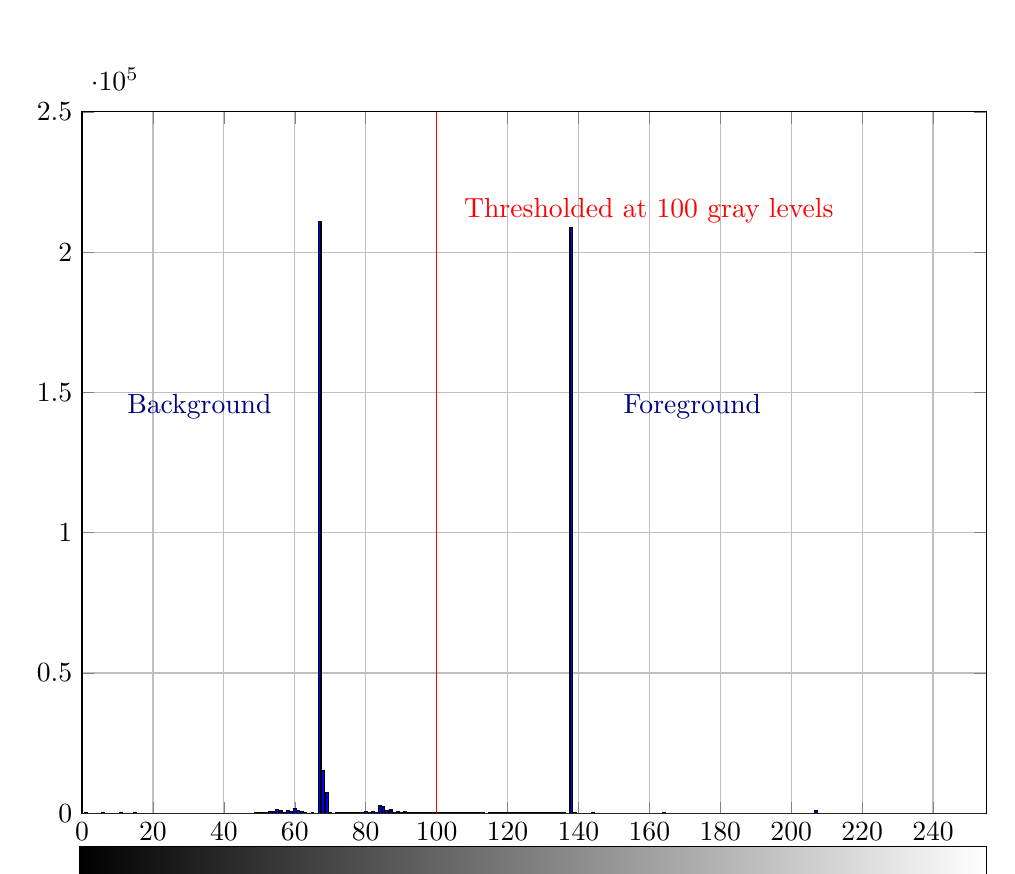
\begin{tikzpicture}	
			\begin{axis}[
			width=4.521in,
			height=3.507in,
			at={(0.758in,0.481in)},
			scale only axis,
			bar shift auto,
			xmin=0,
			xmax=255,
			ymin=0,
			ymax=250000,
			axis background/.style={fill=white},
			title style={},
			title={},
			xmajorgrids,
			ymajorgrids,
			legend style={legend cell align=left, align=left, draw=white!15!black}
			]
			\addplot[ybar, bar width=0.8, fill=blue] table[row sep=crcr] {
				1	103\\
				2	17\\
				3	13\\
				4	13\\
				5	77\\
				6	257\\
				7	16\\
				8	20\\
				9	23\\
				10	41\\
				11	354\\
				12	1\\
				13	1\\
				14	1\\
				15	278\\
				16	1\\
				17	11\\
				18	11\\
				19	17\\
				20	14\\
				21	11\\
				22	18\\
				23	24\\
				24	24\\
				25	40\\
				26	4\\
				27	8\\
				28	2\\
				29	2\\
				30	7\\
				31	13\\
				32	24\\
				33	5\\
				34	17\\
				35	15\\
				36	29\\
				37	15\\
				38	6\\
				39	21\\
				40	18\\
				41	28\\
				42	7\\
				43	17\\
				44	5\\
				45	31\\
				46	65\\
				47	64\\
				48	91\\
				49	184\\
				50	141\\
				51	348\\
				52	272\\
				53	755\\
				54	544\\
				55	1225\\
				56	1105\\
				57	440\\
				58	955\\
				59	636\\
				60	1647\\
				61	1006\\
				62	515\\
				63	394\\
				64	52\\
				65	104\\
				66	56\\
				67	211001\\
				68	15328\\
				69	7494\\
				70	113\\
				71	90\\
				72	152\\
				73	152\\
				74	154\\
				75	172\\
				76	120\\
				77	116\\
				78	102\\
				79	160\\
				80	704\\
				81	329\\
				82	617\\
				83	395\\
				84	2914\\
				85	2330\\
				86	1139\\
				87	1409\\
				88	327\\
				89	771\\
				90	441\\
				91	473\\
				92	192\\
				93	187\\
				94	150\\
				95	163\\
				96	152\\
				97	288\\
				98	210\\
				99	175\\
				100	177\\
				101	163\\
				102	171\\
				103	144\\
				104	133\\
				105	134\\
				106	120\\
				107	121\\
				108	121\\
				109	123\\
				110	114\\
				111	114\\
				112	121\\
				113	99\\
				114	88\\
				115	310\\
				116	110\\
				117	134\\
				118	177\\
				119	196\\
				120	216\\
				121	269\\
				122	260\\
				123	241\\
				124	173\\
				125	163\\
				126	128\\
				127	156\\
				128	149\\
				129	143\\
				130	136\\
				131	127\\
				132	97\\
				133	99\\
				134	105\\
				135	110\\
				136	109\\
				137	92\\
				138	208698\\
				139	99\\
				140	71\\
				141	91\\
				142	79\\
				143	86\\
				144	103\\
				145	84\\
				146	63\\
				147	59\\
				148	48\\
				149	55\\
				150	57\\
				151	66\\
				152	50\\
				153	34\\
				154	46\\
				155	30\\
				156	44\\
				157	26\\
				158	32\\
				159	28\\
				160	20\\
				161	16\\
				162	17\\
				163	18\\
				164	164\\
				165	70\\
				166	18\\
				167	23\\
				168	22\\
				169	18\\
				170	14\\
				171	24\\
				172	0\\
				173	13\\
				174	17\\
				175	0\\
				176	1\\
				177	0\\
				178	0\\
				179	5\\
				180	0\\
				181	1\\
				182	0\\
				183	0\\
				184	0\\
				185	1\\
				186	4\\
				187	13\\
				188	0\\
				189	0\\
				190	0\\
				191	2\\
				192	13\\
				193	1\\
				194	1\\
				195	0\\
				196	7\\
				197	0\\
				198	0\\
				199	2\\
				200	0\\
				201	0\\
				202	0\\
				203	15\\
				204	1\\
				205	3\\
				206	0\\
				207	1015\\
				208	0\\
				209	0\\
				210	1\\
				211	0\\
				212	1\\
				213	0\\
				214	0\\
				215	0\\
				216	0\\
				217	0\\
				218	0\\
				219	0\\
				220	0\\
				221	0\\
				222	0\\
				223	0\\
				224	0\\
				225	0\\
				226	0\\
				227	0\\
				228	0\\
				229	0\\
				230	0\\
				231	0\\
				232	0\\
				233	0\\
				234	0\\
				235	0\\
				236	0\\
				237	0\\
				238	0\\
				239	0\\
				240	0\\
				241	0\\
				242	0\\
				243	0\\
				244	0\\
				245	0\\
				246	0\\
				247	0\\
				248	10\\
				249	2\\
				250	0\\
				251	0\\
				252	0\\
				253	0\\
				254	0\\
				255	0\\
				256	2076\\
			};
			\addplot[forget plot, color=white!15!black] table[row sep=crcr] {
				0	0\\
				255	0\\
			};
			\addplot [color=red] table[row sep=crcr]{
				100	0\\
				100	250000\\
			};
			
			\node[right, align=left, font=\color{red}]
			at (axis cs:105,215000) {Thresholded at 100 gray levels};
			\node[right, align=left, font=\color{black!50!blue}]
			at (axis cs:10,145000) {Background};
			\node[right, align=left, font=\color{black!50!blue}]
			at (axis cs:150,145000) {Foreground};
			\end{axis}
			\filldraw [rectangle, left color=black, right color=white, shading = axis] (13.41,0.8) rectangle (1.9,0.3);
			\end{tikzpicture}
		}
	\end{center}
\end{figure}

\chapter{Drawing on Images}
\label{chapter:drawingOnImages}

\newcounter{drawingOnImages}
\setcounter{drawingOnImages}{0}
\stepcounter{drawingOnImages}

\section{Example \thedrawingOnImages}
\stepcounter{drawingOnImages}

\begin{figure}[H]
	\begin{center}
		\scalebox{1}{
			\begin{tikzpicture}
			
			%Inserisco i nodi che poi conterrano l'immagine
			\node (auto) at (-6,0) [rectangle, minimum width=1cm, minimum height=1cm, label=\textbf{Haar cascade}] {\includegraphics[scale=0.25]{figure/Haar_rilevazione.png}};
			
			\node (auto) at (0,0) [rectangle, minimum width=1cm, minimum height=1cm, label=\textbf{HOG}] {\includegraphics[scale=0.25]{figure/HOG_rilevazione.png}};
			
			\end{tikzpicture}
		}
	\end{center}

\end{figure}

\section{Example \thedrawingOnImages}
\stepcounter{drawingOnImages}

\begin{figure}[H]
	\begin{center}
		\begin{tikzpicture}
		
		%Disegno il sistema di riferimento
		\draw[dashed] (0,0) coordinate -- (0,1.3) coordinate;
		\draw[->] (0,1.3) coordinate -- (0,5) coordinate node[above left]{$Y$};
		\draw[dashed] (0,0) coordinate -- (1.6,0) coordinate;
		\draw[->] (1.6,0) coordinate -- (3,0) coordinate node[above right]{$X$};
		\draw[dashed] (0,0) coordinate -- (-0.5,-0.5) coordinate;
		\draw[->] (-0.5,-0.5) coordinate -- (-2,-2) coordinate node[above left]{$Z$};
		\draw[dashed] (0,0) coordinate -- (1,1) coordinate;
		\draw[-] (1,1) coordinate -- (3,3) coordinate node[below right]{$-Z$};
		\draw[-] (-1.6,0) coordinate -- (-6,0) coordinate;
		
		%Disegno pre proiezioni della camera
		\draw[dashed] (-5,-1) coordinate -- (-5,4) coordinate;
		\draw[dashed] (-4,0) coordinate -- (-5,-1) coordinate;
		\draw[dashed] (-5,-1) coordinate -- (-1,-1) coordinate;
		
		%Disegno l'angolo
		\draw[dashed] (-5,-1) coordinate (a) -- (0,0) coordinate (b) -- (-5,4) coordinate (c)
		pic["$\mathbf{\beta}$", draw, <-, angle eccentricity=1.2, angle radius=2.5cm, line width=1.25pt]{angle=c--b--a};
		
		\draw[dashed] (-4,0) coordinate (d) -- (0,0) coordinate (e);
		
		\draw[dashed] pic["$\mathbf{\alpha}$", draw, ->, angle eccentricity=1.2, angle radius=3.25cm, line width=1.25pt]{angle=d--e--a};
		
		\draw (-3,2.7) coordinate node[above]{$r$};
		
		%Inserisco i nomi
		\draw (-6,5) coordinate node[above]{$\mathbf{Camera}$};
		\draw (2,-1) coordinate node[above left]{$\mathbf{Car}$};
		
		%Inserisco fotocamera ed auto
		%TRIM = sinistra sotto destra sopra
		\node at (-5,5) []{\includegraphics[scale=0.15, trim=17cm 18cm 15cm 45cm]{pdf/Fotocamera.pdf}};
		\node at (2,-1) []{\includegraphics[scale=0.15, trim=17cm 3cm -12cm 45cm]{pdf/Auto.pdf}};
		
		
		\end{tikzpicture}
	\end{center}
	
\end{figure}


\section{Example \thedrawingOnImages}
\stepcounter{drawingOnImages}

\begin{figure}[H]
	\begin{center}
		\scalebox{1}{
			\begin{tikzpicture}
			
			%Rappresento gli angoli sul sistema di riferimento inerziale
			\draw[<-] (0.15,2.3) arc (-25:-110:0.30cm) node[above left]{$\psi$};
			\draw[<-] (-1.9,-1.085) arc (35:-150:0.30cm);
			\draw (-1.7,-1.3) node[below]{$\phi$};
			\draw[<-] (1.8,-1.125) arc (115:-100:0.30cm) node[below right]{$\theta$};
			
			%Inserisco il sistema di riferimento assi-corpo
			\draw[->] (0,0) coordinate -- (0,3) coordinate node[anchor=west]{$u_{z}$};
			\draw[->] (0,0) coordinate -- (-2.5,-1.625) coordinate node[below left]{$u_{x}$};
			\draw[->] (0,0) coordinate -- (2.5,-1.625) coordinate node[below right]{$u_{y}$};
			\draw (-0.05,0.9) node[below right]{$O_{ABC}$};
			
			%Inserisco l'esacottero
			\node (esacottero) at (0,-0.25) [text centered]{\includegraphics[scale=0.15]{figure/esacottero_CAD_trasparente.png}};
			
			%Inserisco gli archi per le Omega
			\draw[<-] (-1.475,-0.385) arc (-25:-100:0.30cm);
			\draw[->] (-1.78,0.7) arc (-35:-110:0.30cm);
			\draw[<-] (-0.365,1.275) arc (-25:-100:0.30cm);
			\draw[->] (1.325,1.175) arc (-45:-110:0.30cm);
			\draw[<-] (2.395,0.3725) arc (-25:-100:0.30cm);
			\draw[->] (1.1625,-0.5725) arc (-25:-100:0.30cm);
			
			%Disegno i vettori delle forze
			\draw[->] (-1.675,-0.685) coordinate -- (-1.675,-0.185) node[left]{$\Omega_1$};
			\draw[->] (-1.98,0.4) coordinate -- (-1.98,0.9) node[left]{$\Omega_6$};
			\draw[->] (-0.565,0.975) coordinate -- (-0.565,1.475) node[left]{$\Omega_5$};
			\draw[->] (1.165,0.875) coordinate -- (1.165,1.375) node[left]{$\Omega_4$};
			\draw[->] (2.195,0.0725) coordinate -- (2.195,0.5725) node[right]{$\Omega_3$};
			\draw[->] (0.9625,-0.9725) coordinate -- (0.9625,-0.4725) coordinate;
			\draw (1.4625,-0.7725) node[above]{$\Omega_2$};
			
			%Rappresento gli angoli sul sistema di riferimento inerziale
			\draw[<-] (-4.3,-1.5) arc (-25:-110:0.30cm) node[left]{$\psi$};
			\draw[<-] (-3.15,-4) arc (55:-110:0.30cm) node[below right]{$\theta$};
			\draw[<-] (-6.1,-3.8) arc (115:-100:0.30cm) node[below right]{$\phi$};
			
			%Inserisco il sistema di riferimento inerziale
			\draw[->] (-4.5,-3) coordinate -- (-4.5,0) coordinate node[anchor=east]{$u_{z}$};
			\draw[->] (-4.5,-3) coordinate -- (-7,-5) coordinate node[below right]{$u_{x}$};
			\draw[->] (-4.5,-3) coordinate -- (-2.5,-5) coordinate node[below left]{$u_{y}$};
			\draw (-4.5,-3) node[right]{$O_{FI}$};
			
			\end{tikzpicture}
		}
	\end{center}
	
\end{figure}

\section{Example \thedrawingOnImages}
\stepcounter{drawingOnImages}

\begin{figure}[H]
	\begin{center}
		\scalebox{1}{
			\begin{tikzpicture}[node distance=2cm]
			
			%Creo i nodi del diagramma di flusso		
			\node (classificatore) at (0,0) [rectangle, draw, text centered, minimum width=2.5cm, minimum height=1cm] {Classifier};
			
			\node (sistemaRiconoscimentoVisi) at (0,-4) [rectangle, draw, text centered, minimum width=2.5cm, minimum height=1cm] {Faces recognition};
			
			\node (endrix) at (-5,-4) [rectangle, minimum width=1cm, minimum height=1cm] {\includegraphics[scale=0.8]{figure/endrix.png}};
			
			\node (endrixRiconosciuto) at (5,-4) [rectangle, minimum width=2cm, minimum height=1cm] {\includegraphics[scale=0.8]{figure/endrixNoto.png}};
			
			\node (falsiPositivi) at (5,1) [rectangle, minimum width=2cm, minimum height=1cm, label=Falsi Positivi] {\includegraphics[scale=1]{figure/falsiPositiviPhoto.png}};
			
			\node (dataSet) at (-5,1) [rectangle, minimum width=2cm, minimum height=1cm, label=Dataset Iniziale] {\includegraphics[scale=0.6]{figure/dataSet.png}};
			
			%Collego i nodi
			\draw [->] (classificatore.south) -- (sistemaRiconoscimentoVisi.north);
			
			\draw [->] (endrix.east) -- (sistemaRiconoscimentoVisi.west);
			
			\draw [->] (endrixRiconosciuto.north) -- (falsiPositivi.south);
			
			\draw [->] (sistemaRiconoscimentoVisi.east) -- (endrixRiconosciuto.west);
			
			\draw [->] (dataSet) to [out=0,in=90] (classificatore);
			\draw [->] (falsiPositivi) to [out=180,in=90] (classificatore);
			
			\end{tikzpicture}
		}
	\end{center}
\end{figure}

\section{Example \thedrawingOnImages}
\stepcounter{drawingOnImages}

\begin{figure}[H]
	\begin{center}
		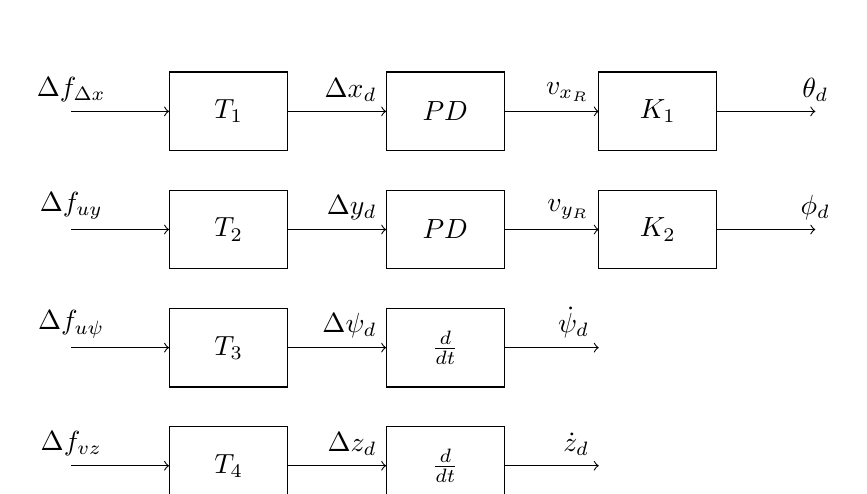
\begin{tikzpicture}
		
		%Disegno i nodi del primo schema
		\node (primaTrasformazione) at (-2,0) [draw, rectangle, minimum width=1.5cm, minimum height=1cm, text centered]{$T_1$};
		
		\node (primoPD) at (0.75,0) [draw, text centered, minimum width=1.5cm, minimum height=1cm]{$PD$};
		
		\node (primoK) at (3.45,0) [draw, text centered, minimum width=1.5cm, minimum height=1cm]{$K_1$};
		
		%Disegno i collegamenti
		\draw[->] (-4,0) coordinate node[above]{$\Delta f_{\Delta x}$} -- (primaTrasformazione.west);
		
		\draw[->] (primaTrasformazione.east) -- (0,0) coordinate node[above left]{$\Delta x_d$};
		
		\draw[->] (primoPD.east) -- (2.7,0) coordinate node[above left]{$v_{{x}_R}$};
		
		\draw[->] (primoK.east) -- (5.45,0) coordinate node[above]{$\theta_d$};
		
		
		%Disegno i nodi del secondo schema
		\node (secondaTrasformazione) at (-2,-1.5) [draw, rectangle, minimum width=1.5cm, minimum height=1cm, text centered]{$T_2$};
		
		\node (secondoPD) at (0.75,-1.5) [draw, text centered, minimum width=1.5cm, minimum height=1cm]{$PD$};
		
		\node (secondoK) at (3.45,-1.5) [draw, text centered, minimum width=1.5cm, minimum height=1cm]{$K_2$};
		
		%Disegno i collegamenti
		\draw[->] (-4,-1.5) coordinate node[above]{$\Delta f_{uy}$} -- (secondaTrasformazione.west);
		
		\draw[->] (secondaTrasformazione.east) -- (0,-1.5) coordinate node[above left]{$\Delta y_d$};
		
		\draw[->] (secondoPD.east) -- (2.7,-1.5) coordinate node[above left]{$v_{{y}_R}$};
		
		\draw[->] (secondoK.east) -- (5.45,-1.5) coordinate node[above]{$\phi_d$};
		
		
		%Disegno i nodi del terzo schema
		\node (terzaTrasformazione) at (-2,-3.0) [draw, rectangle, minimum width=1.5cm, minimum height=1cm, text centered]{$T_3$};
		
		\node (terzoPD) at (0.75,-3.0) [draw, text centered, minimum width=1.5cm, minimum height=1cm]{$\frac{d}{dt}$};
		
		%Disegno i collegamenti
		\draw[->] (-4,-3.0) coordinate node[above]{$\Delta f_{u\psi}$} -- (terzaTrasformazione.west);
		
		\draw[->] (terzaTrasformazione.east) -- (0,-3.0) coordinate node[above left]{$\Delta \psi_d$};
		
		\draw[->] (terzoPD.east) -- (2.7,-3.0) coordinate node[above left]{$\dot{\psi}_d$};
		
		
		%Disegno i nodi il quarto schema
		\node (quartaTrasformazione) at (-2,-4.5) [draw, rectangle, minimum width=1.5cm, minimum height=1cm, text centered]{$T_4$};
		
		\node (quartoPD) at (0.75,-4.5) [draw, text centered, minimum width=1.5cm, minimum height=1cm]{$\frac{d}{dt}$};
		
		%Disegno i collegamenti
		\draw[->] (-4,-4.5) coordinate node[above]{$\Delta f_{vz}$} -- (quartaTrasformazione.west);
		
		\draw[->] (quartaTrasformazione.east) -- (0,-4.5) coordinate node[above left]{$\Delta z_d$};
		
		\draw[->] (quartoPD.east) -- (2.7,-4.5) coordinate node[above left]{$\dot{z}_d$};
		
		
		\end{tikzpicture}
	\end{center}
\end{figure}

\section{Example \thedrawingOnImages}
\stepcounter{drawingOnImages}

\begin{figure}[H]
	\begin{center}
		\begin{tikzpicture}
		
		%Sistema di riferimento inerziale
		\draw[-latex] (0,0) coordinate -- (0,3) coordinate node[above right]{$Y_w$};
		\draw[-latex] (0,0) coordinate -- (3,0) coordinate node[above right]{$X_w$};
		
		%Sistema assi corpo
		\draw[-latex] (5.2,5.2) coordinate -- (7,7) coordinate node[above right]{$X_b$};
		\draw[-latex] (5.2,5.2) coordinate -- (5.2,7.5) coordinate;
		
		%Arco
		\draw (5.2,7.5) coordinate (a) -- (5.2,5.2) coordinate (b) -- (7,7) coordinate (c)
		pic["$\mathbf{\psi}$", draw, latex-, angle eccentricity=1.2, angle radius=1.5cm]{angle=c--b--a};
		
		%Schema drone
		\node (drone) at (4,4) [text centered]{\includegraphics[scale=0.5, angle=-225]{figure/ARDrone_front.png}};
		
		\end{tikzpicture}
	\end{center}
	
\end{figure}

\section{Example \thedrawingOnImages}
\stepcounter{drawingOnImages}

	\begin{figure}[H]
	\begin{center}
		\scalebox{0.85}{			
			\begin{tikzpicture}
			\node (stazioneTerra) at (-4,0) {\includegraphics[scale=0.25]{figure/stazioneTerra.png}};
			\node (drone) at (2.5,0) {\includegraphics[scale=0.2]{figure/droneSnow.png}};
			\node (drone) at (-0.5,2.8) {\includegraphics[scale=0.2]{figure/Freccia_rossa.png}};
			\node (drone) at (-0.5,-2.8) {\includegraphics[scale=0.2]{figure/Freccia_blu.png}};	
			\end{tikzpicture}	
		}
	\end{center}
\end{figure}


\section{Example \thedrawingOnImages}
\stepcounter{drawingOnImages}

\begin{figure}[H]
	\begin{center}
		\begin{tikzpicture}
		\node (grafico) at (0,0) [text centered]{\includegraphics[scale=0.85]{pdf/intro_subsub_msgs}};
		
		\node (cornice1) at (0,2.15) [draw, rectangle, dashed, text centered, red!75, minimum height=4.75cm, minimum width=12cm, line width=2.5pt]{};
		
		\node (cornice2) at (0,-2.75) [draw, rectangle, dashed, text centered, green!75, minimum height=4cm, minimum width=12cm, line width=2.5pt]{};
		\end{tikzpicture}
	\end{center}

\end{figure}

\section{Example \thedrawingOnImages}
\stepcounter{drawingOnImages}

\begin{figure}[H]
	\begin{center}
			\begin{tikzpicture}
			
			%Rappresento gli angoli sul sistema assi-corpo
			\draw[latex-] (0.25,2.3) arc (-25:-110:0.30cm) node[above left]{$\psi$};
			\draw[latex-] (-1.0,-0.9) arc (45:-110:0.30cm);
			\draw (-1.0,-0.9) node[below right]{$\phi$};
			\draw[latex-] (1.825,-0.2) arc (105:-70:0.30cm);
			\draw (2.05,-0.25) node[right]{$\theta$};
			
			%Inserisco il sistema di riferimento assi-corpo
			\draw[-latex] (0.05,0) coordinate -- (0.05,3) coordinate node[anchor=west]{$e_{z}$};
			\draw[-latex] (0.05,0) coordinate -- (-1.60,-1.55) coordinate node[left]{$e_{x}$};
			\draw[-latex] (0.05,-0.1) coordinate -- (2.55,-0.6) coordinate node[below right]{$e_{y}$};
			\draw (0.05,0.8) node[below right]{$O_{ABC}$};
			
			%Inserisco il quadricottero
			\node (esacottero) at (0,0) [text centered]{\includegraphics[scale=0.2]{figure/Crazyflie20_1.png}};
			
			%Inserisco gli archi per le Omega
			\draw[-latex] (-1.3,0.655) arc (55:-15:0.35cm); %omega 1
			\draw[latex-] (-0.05,1.225) arc (-25:-120:0.30cm); %omega 2
			\draw[-latex] (1.2,0.87) arc (55:-15:0.35cm); %omega 3
			\draw[latex-] (0.6225,0.125) arc (-25:-120:0.30cm); %omega 4
			
			%Disegno i vettori delle forze
			\draw[-latex] (-1.225,0.3) coordinate -- (-1.225,0.9) node[left]{$\omega_1$};
			\draw[-latex] (-0.21,0.9) coordinate -- (-0.21,1.5) node[left]{$\omega_2$};
			\draw[-latex] (1.26,0.525) coordinate -- (1.26,1.125) node[right]{$\omega_3$};
			\draw[-latex] (0.36,-0.25) coordinate -- (0.36,0.35) coordinate;
			\draw (0.85,-0.7225) node[above]{$\omega_4$};
			
			%Rappresento gli angoli sul sistema di riferimento inerziale
			\draw[latex-] (-2.9,-2.5) arc (-25:-110:0.30cm) node[left]{$\psi$};
			\draw[latex-] (-2.475,-5.9) arc (105:-70:0.30cm);
			\draw (-2.15,-6.15) node[right]{$\theta$};
			\draw[latex-] (-5.4,-4.9) arc (45:-130:0.30cm);
			\draw (-5.6,-5.3) node[below right]{$\phi$};
			
			%Inserisco il sistema di riferimento inerziale
			\draw[-latex] (-3.05,-5) coordinate -- (-3.05,-2) coordinate node[anchor=east]{$e_{z}$};
			\draw[-latex] (-3.05,-5) coordinate -- (-6.05,-5.275) coordinate node[above right]{$e_{x}$};
			\draw[-latex] (-3.05,-5) coordinate -- (-2.25,-6.725) coordinate node[below left]{$e_{y}$};
			\draw (-3.05,-5) node[right]{$O_{FI}$};
			
			\end{tikzpicture}
	\end{center}
\end{figure} 


\section{Example \thedrawingOnImages}
\stepcounter{drawingOnImages}


	\begin{figure}[H]
	\begin{center}
		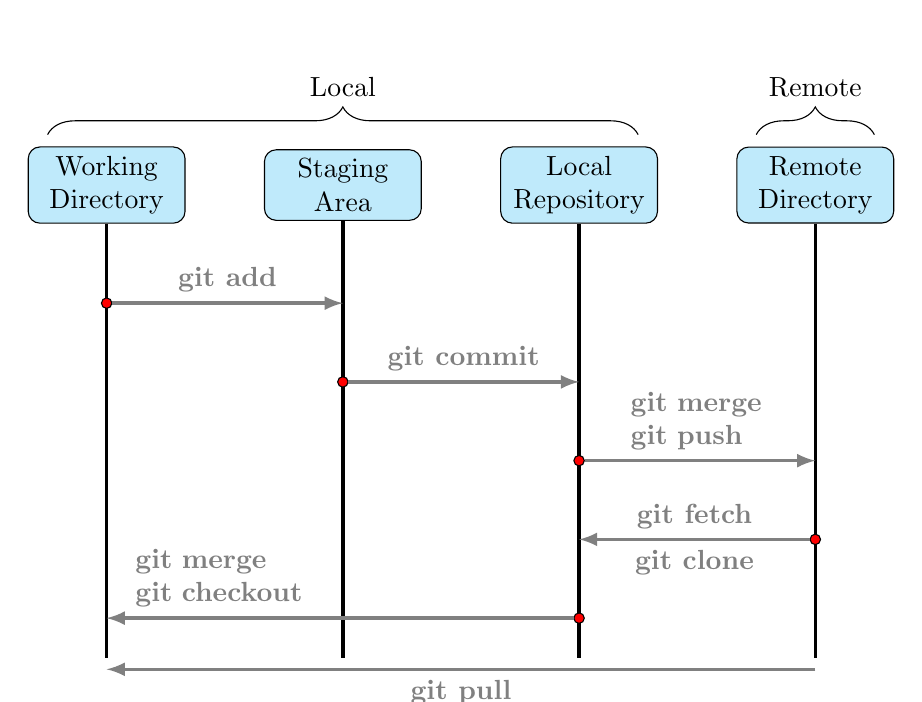
\begin{tikzpicture}
		
		%Rappresento i blocchi
		\node(WorkingDirectory) at (0,0) [rounded corners=0.15cm, draw, minimum width=1.5cm, minimum height=0.75cm, rectangle, text centered, fill=cyan!25, text width=5em]{Working\\Directory};
		\node(StagingArea) at (3,0) [rounded corners=0.15cm, draw, minimum width=1.5cm, minimum height=0.75cm, rectangle, text centered, fill=cyan!25, text width=5em]{Staging\\Area};
		\node(LocalRepository) at (6,0) [rounded corners=0.15cm, draw, minimum width=1.5cm, minimum height=0.75cm, rectangle, text centered, fill=cyan!25, text width=5em]{Local\\Repository};
		\node(RemoteDirectory) at (9,0) [rounded corners=0.15cm, draw, minimum width=1.5cm, minimum height=0.75cm, rectangle, text centered, fill=cyan!25, text width=5em]{Remote\\Directory};
		
		%Rappresento i collegamenti
		\draw[-, line width=1.25pt] (WorkingDirectory.south) -- (0,-6);
		\draw[-, line width=1.25pt] (StagingArea.south) -- (3,-6);
		\draw[-, line width=1.25pt] (LocalRepository.south) -- (6,-6);
		\draw[-, line width=1.25pt] (RemoteDirectory.south) -- (9,-6);
		
		%Inserisco le bubble
		\node (bubble1) at (0,-1.5) [circle, draw, scale=0.4, fill=red]{};
		\node (bubble2) at (3,-2.5) [circle, draw, scale=0.4, fill=red]{};
		\node (bubble3) at (6,-3.5) [circle, draw, scale=0.4, fill=red]{};
		\node (bubble4) at (9,-4.5) [circle, draw, scale=0.4, fill=red]{};
		\node (bubble5) at (6,-5.5) [circle, draw, scale=0.4, fill=red]{};
		
		%Rappresento i collegamenti
		\draw[-latex, gray, line width=1.25pt] (bubble1) -- node[above]{\textbf{git add}} (3,-1.5) coordinate;
		\draw[-latex, gray, line width=1.25pt] (bubble2) -- node[above]{\textbf{git commit}} (6,-2.5) coordinate;
		\draw[-latex, gray, line width=1.25pt] (bubble3) -- node[above, text width=5em]{\textbf{git merge\\git push}} (9,-3.5) coordinate;
		\draw[-latex, gray, line width=1.25pt] (bubble4) -- node[above]{\textbf{git fetch}} node[below]{\textbf{git clone}} (6,-4.5) coordinate;
		\draw[-latex, gray, line width=1.25pt] (bubble5) -- node[above left, text width=7em]{\textbf{git merge\\git checkout}} (0,-5.5) coordinate;
		\draw[-latex, gray, line width=1.25pt] (9,-6.15) coordinate -- node[below]{\textbf{git pull}} (0,-6.15) coordinate;
		
		%Disegno le parentesi graffe - blocco virtual world
		\draw [decorate,decoration={brace, amplitude=10pt,raise=4pt},yshift=0pt] (-0.75,0.5) -- (6.75,0.5) node [black,midway,xshift=0.0cm,yshift=0.75cm] {Local};
		\draw [decorate,decoration={brace, amplitude=10pt,raise=4pt},yshift=0pt] (8.25,0.5) -- (9.75,0.5) node [black,midway,xshift=0.0cm,yshift=0.75cm] {Remote};
		
		\end{tikzpicture}
	\end{center}
\end{figure}

\chapter{Various}
\label{chapter:various}

\newcounter{various}
\setcounter{various}{0}
\stepcounter{various}

\section{Example \thevarious}
\stepcounter{various}

\begin{figure}[h]
	\begin{center}
		\scalebox{0.5}{
			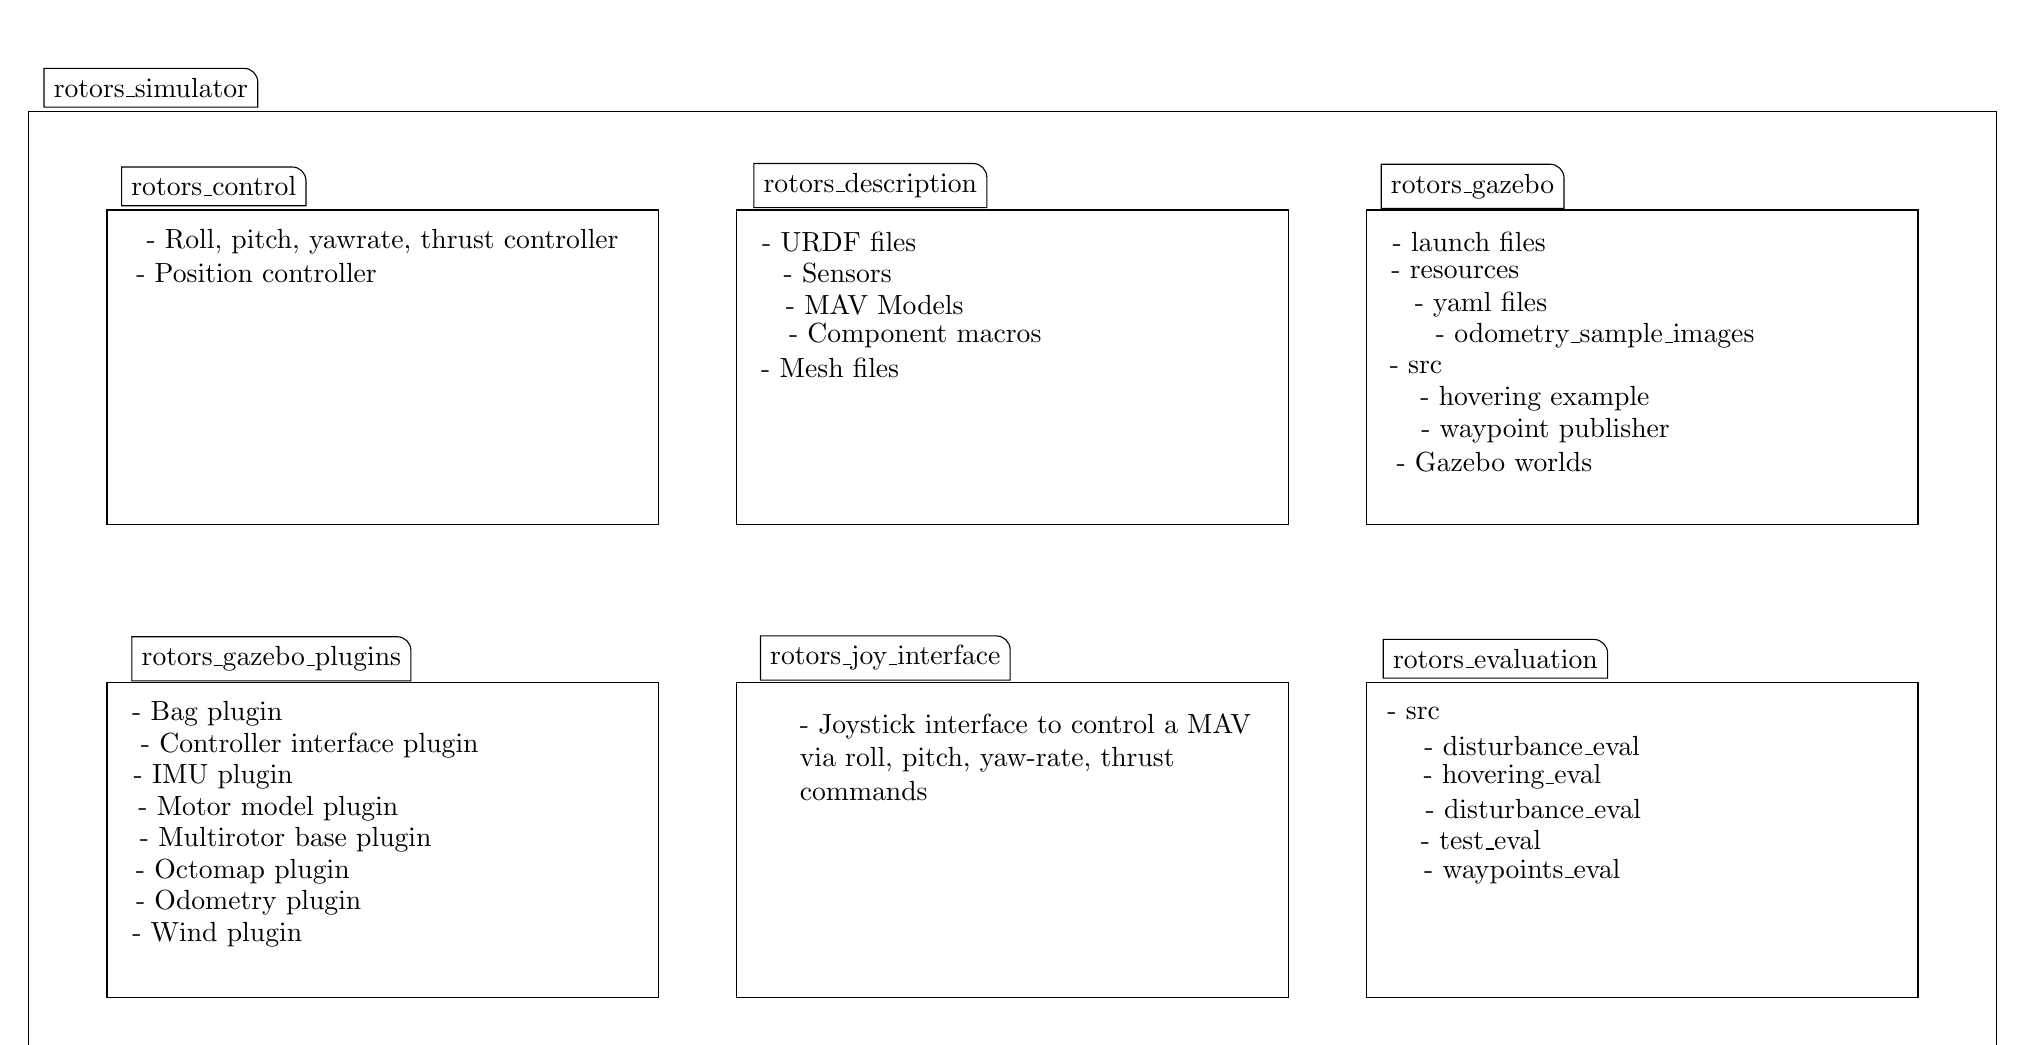
\begin{tikzpicture}
			
			%Package comments
			\node (Rotors Control) at (0,0) [draw, rectangle, minimum height=4cm, minimum 
			width=7cm, text centered]{};
			\draw node at (-2.1435,2.3)[
			append after command={[rounded corners=0pt](b.west)|-(b.north)},
			append after command={[rounded corners=5pt](b.north)-|(b.east)},
			append after command={[rounded corners=0pt](b.east)|-(b.south)},
			append after command={[rounded corners=0pt](b.south)-|(b.west)}] 
			(b) {rotors\_control};
			
			%Writing in the box
			\node at (0,1.6) [text centered]{- Roll, pitch, yawrate, thrust controller};
			\node at (-1.6,1.2) [text centered]{- Position controller};
			
			%Second block
			\node (Rotors Description) at (8,0) [draw, rectangle, minimum height=4cm, minimum 
			width=7cm, text centered]{};
			\draw node at (6.195,2.31)[
			append after command={[rounded corners=0pt](b.west)|-(b.north)},
			append after command={[rounded corners=5pt](b.north)-|(b.east)},
			append after command={[rounded corners=0pt](b.east)|-(b.south)},
			append after command={[rounded corners=0pt](b.south)-|(b.west)}] 
			(b) {rotors\_description};
			
			%Writing in the box
			\node at (5.8,1.6) [text centered]{- URDF files};
			\node at (5.78,1.2) [text centered]{- Sensors};
			\node at (6.25,0.8) [text centered]{- MAV Models};
			\node at (6.765,0.4) [text centered]{- Component macros};
			\node at (5.685,0) [text centered]{- Mesh files};
			
			%Third block
			\node (Rotors Gazebo) at (16,0) [draw, rectangle, minimum height=4cm, minimum 
			width=7cm, text centered]{};
			\draw node at (13.8435,2.3)[
			append after command={[rounded corners=0pt](b.west)|-(b.north)},
			append after command={[rounded corners=5pt](b.north)-|(b.east)},
			append after command={[rounded corners=0pt](b.east)|-(b.south)},
			append after command={[rounded corners=0pt](b.south)-|(b.west)}] 
			(b) {rotors\_gazebo};
			
			%Writing in the box
			\node at (13.8,1.6) [text centered]{- launch files};
			\node at (13.625,1.2) [text centered]{- resources};
			\node at (13.95,0.8) [text centered]{- yaml files};
			\node at (15.4,0.4) [text centered]{- odometry\_sample\_images};
			\node at (13.125,0.0) [text centered]{- src};
			\node at (14.635,-0.4) [text centered]{- hovering example};
			\node at (14.77,-0.8) [text centered]{- waypoint publisher};
			\node at (14.12,-1.2) [text centered]{- Gazebo worlds};
			
			%Fourth block
			\node (Rotors Control) at (0,-6) [draw, rectangle, minimum height=4cm, minimum 
			width=7cm, text centered]{};
			\draw node at (-1.4115,-3.7)[
			append after command={[rounded corners=0pt](b.west)|-(b.north)},
			append after command={[rounded corners=5pt](b.north)-|(b.east)},
			append after command={[rounded corners=0pt](b.east)|-(b.south)},
			append after command={[rounded corners=0pt](b.south)-|(b.west)}] 
			(b) {rotors\_gazebo\_plugins};
			
			%Writing in the box
			\node at (-2.225,-4.4) [text centered]{- Bag plugin};
			\node at (-0.925,-4.8) [text centered]{- Controller interface plugin};
			\node at (-2.15,-5.2) [text centered]{- IMU plugin};
			\node at (-1.45,-5.6) [text centered]{- Motor model plugin};
			\node at (-1.23,-6.0) [text centered]{- Multirotor base plugin};
			\node at (-1.775,-6.4) [text centered]{- Octomap plugin};
			\node at (-1.7,-6.8) [text centered]{- Odometry plugin};
			\node at (-2.1,-7.2) [text centered]{- Wind plugin};
			
			
			%Fifth block
			\node (Rotors Joy Interface) at (8,-6) [draw, rectangle, minimum height=4cm, minimum 
			width=7cm, text centered]{};
			\draw node at (6.385,-3.69)[
			append after command={[rounded corners=0pt](b.west)|-(b.north)},
			append after command={[rounded corners=5pt](b.north)-|(b.east)},
			append after command={[rounded corners=0pt](b.east)|-(b.south)},
			append after command={[rounded corners=0pt](b.south)-|(b.west)}] 
			(b) {rotors\_joy\_interface};
			
			%Writing in the box
			\node at (11.45,-4.95) [text width=35em]{- Joystick interface to control a MAV\\via 
			roll, pitch, yaw-rate, thrust\\commands};
			
			%Sixth block
			\node (Rotors Evaluation) at (16,-6) [draw, rectangle, minimum height=4cm, minimum 
			width=7cm, text centered]{};
			\draw node at (14.1335,-3.70)[
			append after command={[rounded corners=0pt](b.west)|-(b.north)},
			append after command={[rounded corners=5pt](b.north)-|(b.east)},
			append after command={[rounded corners=0pt](b.east)|-(b.south)},
			append after command={[rounded corners=0pt](b.south)-|(b.west)}] 
			(b) {rotors\_evaluation};
			
			%Writing in the box
			\node at (13.095,-4.4) [text centered]{- src};
			\node at (14.6,-4.8) [text centered]{- disturbance\_eval};
			\node at (14.35,-5.2) [text centered]{- hovering\_eval};
			\node at (14.615,-5.6) [text centered]{- disturbance\_eval};
			\node at (13.95,-6.0) [text centered]{- test\_eval};
			\node at (14.475,-6.4) [text centered]{- waypoints\_eval};
			
			%Container
			\node (container) at (8,-2.75) [draw, rectangle, minimum height=12cm, minimum 
			width=25cm]{};
			\draw node at (-2.9421,3.5525)[
			append after command={[rounded corners=0pt](b.west)|-(b.north)},
			append after command={[rounded corners=5pt](b.north)-|(b.east)},
			append after command={[rounded corners=0pt](b.east)|-(b.south)},
			append after command={[rounded corners=0pt](b.south)-|(b.west)}] 
			(b) {rotors\_simulator};
			
			\end{tikzpicture}
		}
	\end{center}

\end{figure}

\section{Example \thevarious}
\stepcounter{various}

\begin{figure}[h]
	\begin{center}
		\scalebox{0.8}{
		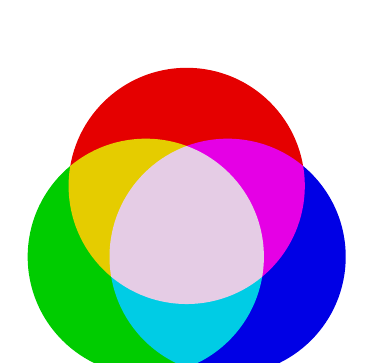
\begin{tikzpicture}[blend group=screen]
		\fill[red!90!black]   ( 90:.6) circle (1.5);
		\fill[green!80!black] (210:.6) circle (1.5);
		\fill[blue!90!black] (330:.6) circle (1.5);
		\end{tikzpicture}
	}
	\end{center}
\end{figure}

\newpage


\section{Example \thevarious}
\stepcounter{various}

\begin{figure}[h]
	\begin{center}
		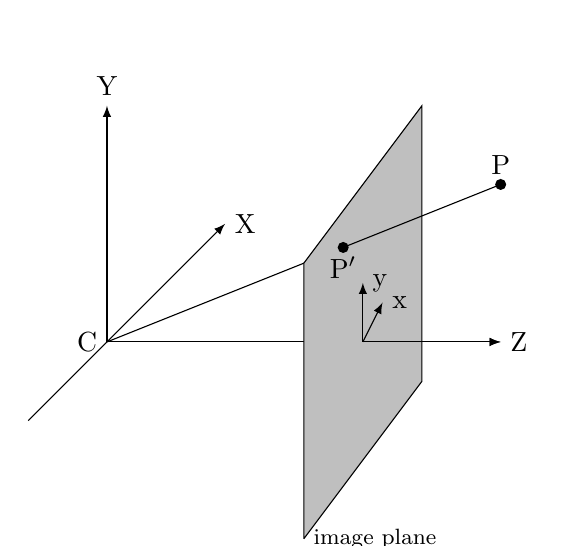
\begin{tikzpicture}
		
		\draw[-latex] (0,0) node[anchor=east]{C} -- (5,0) node[anchor=west] {Z};
		\draw[-latex] (0,0) -- (0,3) node[anchor=south] {Y};
		\draw[-latex] (-1.0,-1.0) -- (1.5,1.5) node[anchor=west] {X};
		\draw (0,0) -- (3,1.2);
		\filldraw[fill=lightgray] (2.5,-2.5) -- (2.5,1) --  (4,3) -- (4,-0.5) -- (2.5,-2.5);
		\draw[-latex] (3.25,0) -- (3.25,0.75) node[anchor=west] {y};
		\draw[-latex] (3.25,0) -- (3.5,0.5) node[anchor=west] {x};
		\draw[-latex] (3.25,0) -- (5,0);
		\draw (3,1.2) -- (5,2);
		\fill (5,2) circle[radius=2pt] node[anchor=south] {P};
		\fill (3,1.2) circle[radius=2pt] node[anchor=north] {P$'$};
		\draw (2.5,-2.5) node[anchor=west, font=\footnotesize] {image plane};
		
		\end{tikzpicture}
	\end{center}
	
\end{figure}


\section{Example \thevarious}
\stepcounter{various}

\begin{figure}[h]
	\begin{center}
		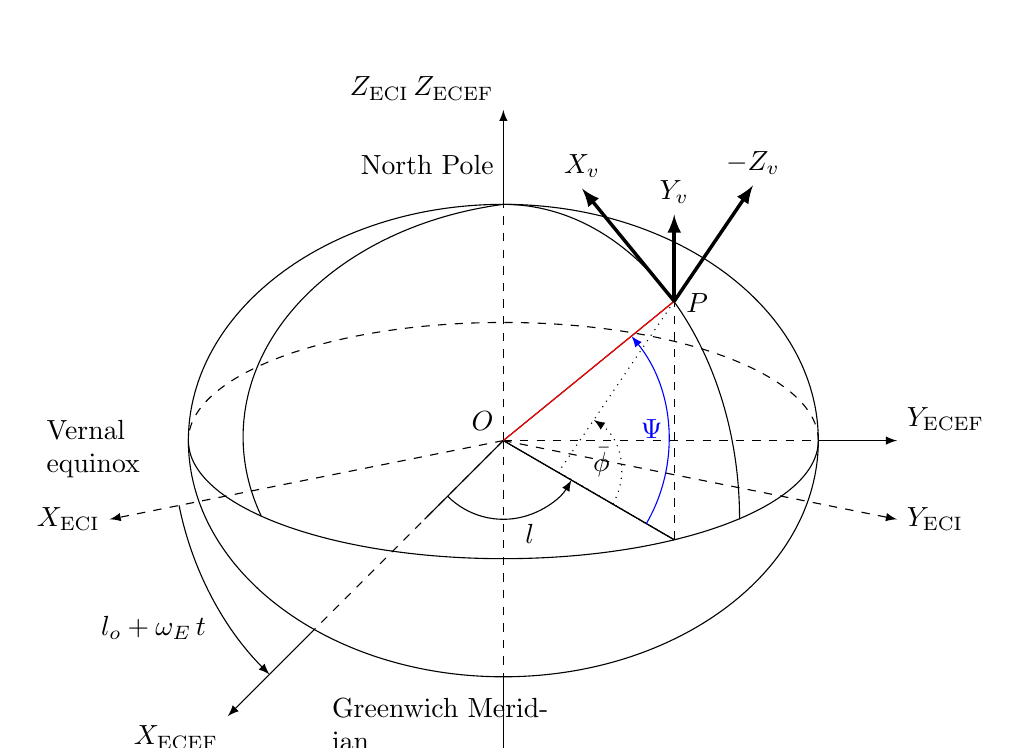
\begin{tikzpicture}
		
		%Reference system
		\draw[dashed] (0,0) coordinate -- (0,3) coordinate;
		\draw[-latex] (0,3) coordinate -- (0,4.2) coordinate node[above 
		left]{$Z_\mathrm{ECI}\,Z_\mathrm{ECEF}$};
		\draw (0,3.25) node[above left]{North Pole};
		\draw[dashed] (0,0) coordinate -- (-2.45,-2.45) coordinate;
		\draw[-latex] (-2.45,-2.45) coordinate -- (-3.5,-3.5) coordinate node [below 
		left]{$X_\mathrm{ECEF}$};
		\draw[-latex, dashed] (0,0) coordinate -- (-5,-1) coordinate node[left]{$X_\mathrm{ECI}$};
		\draw (-2.3,-3.6) node[right, text width=3cm]{Greenwich Meridian};
		\draw[dashed] (0,0) coordinate -- (4,0);
		\draw[-latex] (4,0) coordinate -- (5,0) coordinate node [above right]{$Y_\mathrm{ECEF}$};
		\draw[-latex, dashed] (0,0) coordinate -- (5.0,-1) coordinate node[right]{$Y_\mathrm{ECI}$};
		\draw (-4.8,-0.6) node[above, text width=2cm]{Vernal equinox};
		
		%First line and angle
		\draw[-] (-1,-1) coordinate (a) -- (0,0) coordinate (b) -- (2.17,-1.26) coordinate (c)
		pic[right,"$l$", draw, -latex, angle eccentricity=1.2, angle radius=1cm]{angle=a--b--c};
		
		%Second line and angle
		\draw[dotted] (2.17,-1.26) coordinate (d) -- (0.70,-0.40) coordinate (e) -- (2.17,1.77) 
		coordinate (f)
		pic["$\bar{\phi}$", draw, -latex, angle eccentricity=0.7, angle 
		radius=0.8cm]{angle=d--e--f};
		
		%Third line and angle
		\draw[-] (2.17,-1.26) coordinate (g) -- (0,0) coordinate (h) -- (2.17,1.77) coordinate (i)
		pic["$\Psi$", draw, blue, -latex, angle eccentricity=0.9, angle 
		radius=2.1cm]{angle=g--h--i};
		
		%Fourth line and angle
		\coordinate (l) at (-5,-1);
		\coordinate (m) at (0,0); 
		\coordinate (n) at (-3.5,-3.5);
		\draw pic["$l_o+\omega_E\,t$", draw, -latex, angle eccentricity=1.2, angle 
		radius=4.2cm]{angle=l--m--n};
		
		%Horizontal axis
		\draw (0,0) ellipse (4cm and 3cm);
		
		%Vertical ellipse
		\draw[dashed] (4,0) arc (0:180:4cm and 1.5cm);
		\draw (-4,0) arc (180:360:4cm and 1.5cm);
		
		%Arcs
		\draw[] (0,3) arc (100:199.5:4cm and 3cm);
		\draw (0,3) arc (90:0):3cm and 4cm);
		
		%Z-axis dashed
		\draw[dashed] (0,0) coordinate -- (0,-3) coordinate;
		\draw (0,-3) coordinate -- (0,-4) coordinate;
		
		%Reference system origin
		\draw (0,0) coordinate node[above left]{$O$};
		\draw[-, red] (0,0) coordinate -- (2.17,1.77) coordinate;
		\draw (2.2,1.5) coordinate node[above right]{$P$};
		\draw[dashed] (2.17,-1.26) coordinate -- (2.17,1.77) coordinate;
		
		%Second reference system
		\draw[-latex,line width=1.25pt] (2.17,1.77) coordinate -- (3.17,3.24) coordinate 
		node[above]{$-Z_v$};
		\draw[-latex,line width=1.25pt] (2.17,1.77) coordinate -- (1,3.2) coordinate 
		node[above]{$X_v$};
		\draw[-latex,line width=1.25pt] (2.17,1.77) coordinate -- (2.17,2.87) coordinate 
		node[above]{$Y_v$};
		
		\end{tikzpicture}
	\end{center}
	
\end{figure}

\newpage


\section{Example \thevarious}
\stepcounter{various}

\begin{figure}[h]
	\begin{center}
		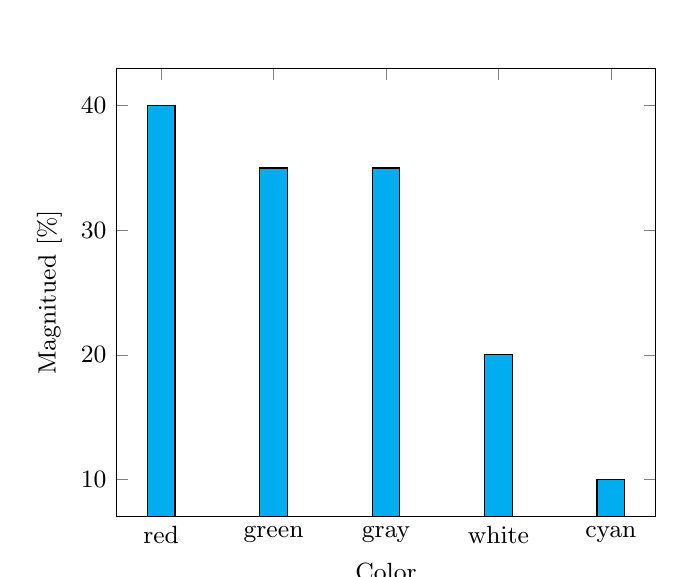
\begin{tikzpicture}[font=\small]
		
		%Histogram
		\begin{axis}[
		symbolic x coords={red, green, gray, white, cyan},
		ylabel = {Magnitued [$\%$]},
		xlabel = {Color},
		xtick=data
		]
		\addplot[ybar,draw=black, fill=cyan] coordinates {
			(red,  40)
			(green,  35)
			(gray, 35)
			(white, 20)
			(cyan,  10)
		};
		\end{axis}
		
		\end{tikzpicture}
	\end{center}
	
\end{figure}


\section{Example \thevarious}
\stepcounter{various}

\begin{figure}[h]
	\begin{center}
		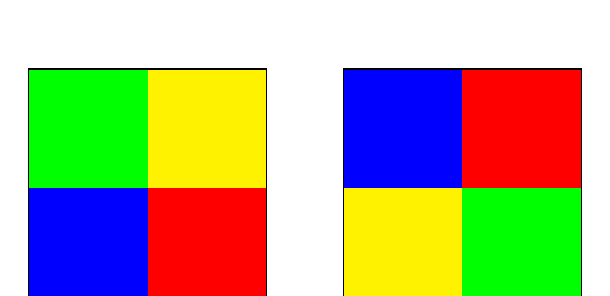
\begin{tikzpicture}
		
		%First squre
		\node (square) at (-2,0) [rectangle, draw, minimum width=3cm, minimum height=3cm, text 
		centered, line width=1.25pt]{};
		
		%Square divider
		\node (firstLine) at (-2.75, 0.75) [rectangle, fill=green, minimum width=1.5cm, minimum 
		height=1.5cm, text centered]{};
		\node (secondLine) at (-1.25, 0.75) [rectangle, fill=yellow, minimum width=1.5cm, minimum 
		height=1.5cm, text centered]{};
		\node (thirdLine) at (-2.75, -0.75) [rectangle, fill=blue, minimum width=1.5cm, minimum 
		height=1.5cm, text centered]{};
		\node (fourthLine) at (-1.25, -0.75) [rectangle, fill=red, minimum width=1.5cm, minimum 
		height=1.5cm, text centered]{};
		
		%Second squre
		\node (square2) at (2,0) [rectangle, draw, minimum width=3cm, minimum height=3cm, text 
		centered, line width=1.25pt]{};
		
		%Square divider
		\node (firstLine1) at (2.75, 0.75) [rectangle, fill=red, minimum width=1.5cm, minimum 
		height=1.5cm, text centered]{};
		\node (secondLine1) at (1.25, 0.75) [rectangle, fill=blue, minimum width=1.5cm, minimum 
		height=1.5cm, text centered]{};
		\node (thirdLine1) at (2.75, -0.75) [rectangle, fill=green, minimum width=1.5cm, minimum 
		height=1.5cm, text centered]{};
		\node (fourthLine1) at (1.25, -0.75) [rectangle, fill=yellow, minimum width=1.5cm, minimum 
		height=1.5cm, text centered]{};
		
		\end{tikzpicture}
	\end{center}
	
\end{figure}



\section{Example \thevarious}
\stepcounter{various}

\begin{figure}[h]
	\begin{center}
		\scalebox{0.8}{
		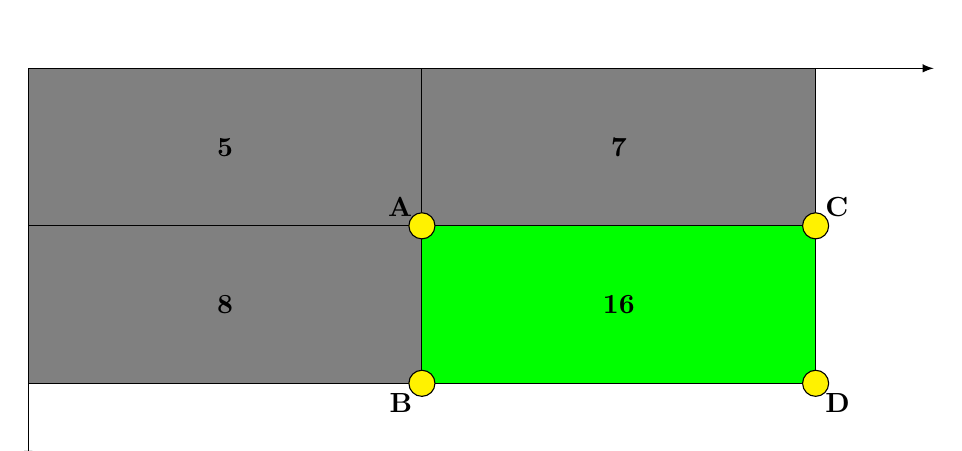
\begin{tikzpicture}
		
		%Squares
		\node (firstSquare) at (-5,5) [rectangle, draw, text centered, text width=6em, minimum 
		width=5cm, minimum height=2cm, fill=gray] {\textbf{5}};
		\node (secondSquare) at (0,5) [rectangle, draw, text centered, text width=6em, minimum 
		width=5cm, minimum height=2cm, fill=gray] {\textbf{7}};
		\node (thirdSquare) at (-5,3) [rectangle, draw, text centered, text width=6em, minimum 
		width=5cm, minimum height=2cm, fill=gray] {\textbf{8}};
		\node (fourthSquare) at (0,3) [rectangle, draw, text centered, text width=6em, minimum 
		width=5cm, minimum height=2cm, fill=green] {\textbf{16}};
		
		%Circles
		\node (firstCircle) at (-2.5,4) [circle, draw, text centered, minimum size=0.2cm, 
		fill=yellow]{};
		\node (secondCircle) at (-2.5,2) [circle, draw, text centered, minimum size=0.2cm, 
		fill=yellow]{};
		\node (thirdCircle) at (2.5,4) [circle, draw, text centered, minimum size=0.2cm, 
		fill=yellow]{};
		\node (fourthCircle) at (2.5,2) [circle, draw, text centered, minimum size=0.2cm, 
		fill=yellow]{};
		
		%Axes
		\draw[-latex] (-7.5,6) coordinate -- (4,6) coordinate;
		\draw[-latex] (-7.5,6) coordinate -- (-7.5,1) coordinate;
		
		%Letters
		\draw (-2.5, 4) coordinate node[above left]{\textbf{A}};
		\draw (2.5, 4) coordinate node[above right]{\textbf{C}};
		\draw (-2.5, 2) coordinate node[below left]{\textbf{B}};
		\draw (2.5, 2) coordinate node[below right]{\textbf{D}};
		
		\end{tikzpicture}
	}
	\end{center}
	
\end{figure}

\newpage

\section{Example \thevarious}
\stepcounter{various}

\begin{figure}[h]
	\begin{center}
		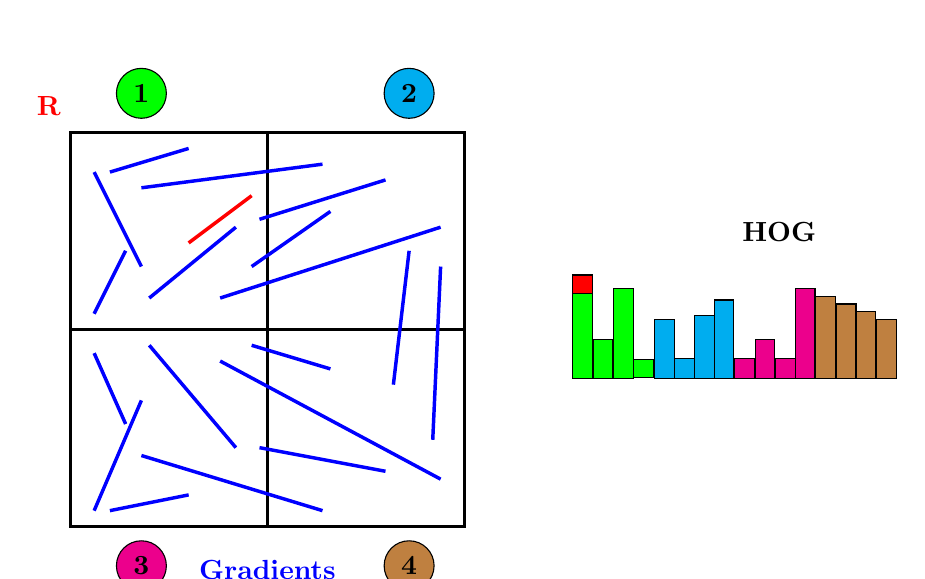
\begin{tikzpicture}
		
		%First squre
		\node (square) at (-5,0) [rectangle, draw, minimum width=5cm, minimum height=5cm, text 
		centered, line width=1.25pt]{};
		
		%Square divider
		\draw[-, line width=1.25pt] (-5,2.5) coordinate -- (-5, -2.5) coordinate;
		\draw[-, line width=1.25pt] (-7.5,0) coordinate -- (-2.5,0);
		
		%Lines
		\draw[-, blue, line width=1.25pt] (-7.2,0.2) coordinate -- (-6.8,1.0) coordinate;
		\draw[-, blue, line width=1.25pt] (-6.5, 0.4) coordinate -- (-5.4, 1.3) coordinate;
		\draw[-, blue, line width=1.25pt] (-6.6, 0.8) coordinate -- (-7.2, 2.0) coordinate;
		\draw[-, blue, line width=1.25pt] (-5.6, 0.4) coordinate -- (-2.8, 1.3) coordinate;
		\draw[-, blue, line width=1.25pt] (-5.2, 0.8) coordinate -- (-4.2, 1.5) coordinate;
		\draw[-, blue, line width=1.25pt] (-5.1, 1.4) coordinate -- (-3.5, 1.9) coordinate;
		\draw[-, blue, line width=1.25pt] (-7.0, 2.0) coordinate -- (-6.0, 2.3) coordinate;
		\draw[-, blue, line width=1.25pt] (-6.6, 1.8) coordinate -- (-4.3, 2.1) coordinate;
		
		\draw[-, blue, line width=1.25pt] (-7.2,-0.3) coordinate -- (-6.8, -1.2) coordinate;
		\draw[-, blue, line width=1.25pt] (-6.5, -0.2) coordinate -- (-5.4, -1.5) coordinate;
		\draw[-, blue, line width=1.25pt] (-6.6, -0.9) coordinate -- (-7.2, -2.3) coordinate;
		\draw[-, blue, line width=1.25pt] (-5.6, -0.4) coordinate -- (-2.8, -1.9) coordinate;
		\draw[-, blue, line width=1.25pt] (-5.2, -0.2) coordinate -- (-4.2, -0.5) coordinate;
		\draw[-, blue, line width=1.25pt] (-5.1, -1.5) coordinate -- (-3.5, -1.8) coordinate;
		\draw[-, blue, line width=1.25pt] (-7.0, -2.3) coordinate -- (-6.0, -2.1) coordinate;
		\draw[-, blue, line width=1.25pt] (-6.6, -1.6) coordinate -- (-4.3, -2.3) coordinate;
		
		\draw[-, blue, line width=1.25pt] (-2.8, 0.8) coordinate -- (-2.9, -1.4) coordinate;
		\draw[-, blue, line width=1.25pt] (-3.2, 1.0) coordinate -- (-3.4, -0.7) coordinate;
		
		\draw[-, red, line width=1.25pt] (-6.0, 1.1) coordinate -- (-5.2, 1.7) coordinate;
		
		%Histogram
		\node (rectangle1) at (-1,-0.05) [rectangle, draw, minimum width=0.25cm, fill=green, 
		minimum height=1.15cm, text centered]{};
		\node (rectangle) at (-1,0.575) [rectangle, draw, minimum width=0.25cm, fill=red, minimum 
		height=0.15cm, text centered]{};
		\node (rectangle2) at (-0.74,-0.375) [rectangle, draw, fill=green, minimum width=0.25cm, 
		minimum height=0.5cm, text centered]{};
		\node (rectangle3) at (-0.48,-0.05) [rectangle, draw, fill=green, minimum width=0.25cm, 
		minimum height=1.15cm, text centered]{};
		\node (rectangle4) at (-0.22,-0.497) [rectangle, draw, fill=green, minimum width=0.25cm, 
		minimum height=0.15cm, text centered]{};
		\node (rectangle5) at (0.04,-0.25) [rectangle, draw, fill=cyan, minimum width=0.25cm, 
		minimum height=0.75cm, text centered]{};
		\node (rectangle6) at (0.30,-0.497) [rectangle, draw, fill=cyan, minimum width=0.25cm, 
		minimum height=0.25cm, text centered]{};
		\node (rectangle7) at (0.55,-0.225) [rectangle, draw, fill=cyan, minimum width=0.25cm, 
		minimum height=0.80cm, text centered]{};
		\node (rectangle8) at (0.80,-0.125) [rectangle, draw, fill=cyan, minimum width=0.25cm, 
		minimum height=1.00cm, text centered]{};
		\node (rectangle9) at (1.06,-0.497) [rectangle, draw, minimum width=0.25cm, fill=magenta, 
		minimum height=0.25cm, text centered]{};
		\node (rectangle10) at (1.32,-0.375) [rectangle, draw, fill=magenta, minimum width=0.25cm, 
		minimum height=0.5cm, text centered]{};
		\node (rectangle11) at (1.58,-0.497) [rectangle, draw, fill=magenta, minimum width=0.25cm, 
		minimum height=0.25cm, text centered]{};
		\node (rectangle12) at (1.83,-0.05) [rectangle, draw, fill=magenta, minimum width=0.25cm, 
		minimum height=1.15cm, text centered]{};
		\node (rectangle13) at (2.09,-0.1) [rectangle, draw, fill=brown, minimum width=0.25cm, 
		minimum height=1.05cm, text centered]{};
		\node (rectangle14) at (2.35,-0.15) [rectangle, draw, fill=brown, minimum width=0.25cm, 
		minimum height=0.95cm, text centered]{};
		\node (rectangle15) at (2.60,-0.2) [rectangle, draw, fill=brown, minimum width=0.25cm, 
		minimum height=0.85cm, text centered]{};
		\node (rectangle16) at (2.86,-0.25) [rectangle, draw, fill=brown, minimum width=0.25cm, 
		minimum height=0.75cm, text centered]{};
		
		%Names
		\draw (1.5, 1.0) coordinate node[above]{\textbf{HOG}};
		\draw[blue] (-5,-2.8) coordinate node[below]{\textbf{Gradients}};
		\draw[red] (-7.5,2.6) node[above left]{\textbf{R}};
		
		%Circles
		\node (firstCircle) at (-6.6,3.0) [circle, draw, text centered, minimum size=0.2cm, 
		fill=green]{\textbf{1}};
		\node (secondCircle) at (-3.2,3.0) [circle, draw, text centered, minimum size=0.2cm, 
		fill=cyan]{\textbf{2}};
		\node (thirdCircle) at (-6.6,-3.0) [circle, draw, text centered, minimum size=0.2cm, 
		fill=magenta]{\textbf{3}};
		\node (fourthCircle) at (-3.2,-3.0) [circle, draw, text centered, minimum size=0.2cm, 
		fill=brown]{\textbf{4}};
		
		\end{tikzpicture}
	\end{center}
\end{figure}



\section{Example \thevarious}
\stepcounter{various}

\begin{figure}[h]
	\begin{center}
		\scalebox{0.9}{
		\begin{tikzpicture}
		
		%First square
		\node (firstSquare) at (-3,5) [rectangle, draw, text centered, minimum width=4cm, minimum 
		height=4cm]{};
		
		\node (firstSubSquare1) at (-4,5) [rectangle, draw, text centered, minimum width=1cm, 
		minimum height=3cm]{};
		\node (secondSubSquare1) at (-3,5) [rectangle, draw, text centered, minimum width=1cm, 
		minimum height=3cm, fill=gray]{};
		
		\draw (-2.5, 3.8) coordinate node[below right]{\textbf{A}};
		
		%Second square
		\node (secondSquare) at (3,5) [rectangle, draw, text centered, minimum width=4cm, minimum 
		height=4cm]{};
		
		\node (firstSubSquare2) at (3.5,6) [rectangle, draw, text centered, minimum width=2cm, 
		minimum height=1cm]{};
		\node (secondSubSquare2) at (3.5,5) [rectangle, draw, text centered, minimum width=2cm, 
		minimum height=1cm, fill=gray]{};
		
		\draw (2.6, 4.5) coordinate node[below left]{\textbf{B}};
		
		%Third square
		\node (thirdSquare) at (-3,0) [rectangle, draw, text centered, minimum width=4cm, minimum 
		height=4cm]{};
		
		\node (firstSubSquare3) at (-4,-1) [rectangle, draw, text centered, minimum width=1cm, 
		minimum height=1.2cm]{};
		\node (secondSubSquare3) at (-3,-1) [rectangle, draw, text centered, minimum width=1cm, 
		minimum height=1.2cm, fill=gray]{};
		\node (thirdSubSquare3) at (-2,-1) [rectangle, draw, text centered, minimum width=1cm, 
		minimum height=1.2cm]{};
		
		\draw (-4.2, -0.4) coordinate node[above left]{\textbf{C}};
		
		%Fourth square
		\node (fourthSquare) at (3,0) [rectangle, draw, text centered, minimum width=4cm, minimum 
		height=4cm]{};
		
		\node (firstSubSquare4) at (3.5,1) [rectangle, draw, text centered, minimum width=1cm, 
		minimum height=1.5cm]{};
		\node (secondSubSquare4) at (2.5,1) [rectangle, draw, text centered, minimum width=1cm, 
		minimum height=1.5cm, fill=gray]{};
		\node (thirdSubSquare4) at (3.5,-0.5) [rectangle, draw, text centered, minimum width=1cm, 
		minimum height=1.5cm, fill=gray]{};
		\node (fourthSubSquare4) at (2.5,-0.5) [rectangle, draw, text centered, minimum width=1cm, 
		minimum height=1.5cm]{};
		
		\draw (2.2, -1.3) coordinate node[below left]{\textbf{D}};
		
		\end{tikzpicture}
	}
	\end{center}
	
\end{figure}

\newpage


\section{Example \thevarious}
\stepcounter{various}

\begin{figure}[h]
	\begin{center}
		\begin{tikzpicture}
		
		%Reference System
		\draw[-latex, draw, dashed] (3.33,0) coordinate -- (4,0) coordinate node[below right]{$x$};
		\draw[draw, dashed] (0,0) coordinate -- (0,2.25) coordinate;
		\draw[-latex, draw, dashed] (0,2.25) coordinate -- (0,3) coordinate (asse) node[below 
		right]{$y$};
		
		%Circles
		\node[circle,draw,black,minimum size=0.5cm] (A) at (2,2){1};	
		\node[circle,draw,black,minimum size=0.5cm] (B) at (-2,2){6};
		\node[circle,draw,black,minimum size=0.5cm] (C) at (-3,0){5};
		\node[circle,draw,black,minimum size=0.5cm] (D) at (-2,-2){4};
		\node[circle,draw,black,minimum size=0.5cm] (E) at (2,-2){3};
		\node[circle, draw, fill=black, scale=0.5] (center) at (0,0){} pic["$\beta$", draw, <-, 
		angle eccentricity=1.2, angle radius=1.5cm, line width=1.0pt]{angle=B--center--C};
		\node[circle,draw,black,minimum size=0.5cm] (F) at (3,0){2} pic["$\alpha$", draw, <-, angle 
		eccentricity=1.2, angle radius=1.5cm, line width=1.0pt]{angle=A--center--asse};
		
		%Arm links
		\draw[line width=0.5pt] (C.east) -- (F.west);
		\draw[line width=0.5pt] (B.315) -- (0,0) coordinate;
		\draw[line width=0.5pt] (D.45) -- (0,0) coordinate;
		\draw[line width=0.5pt] (E.135) -- (0,0) coordinate;
		\draw[line width=0.5pt] (A.235) -- (0,0) coordinate;
		
		%Angles
		\draw[thick,-latex] ([shift=(20:0.5cm)]2,2) arc (20:50:1cm);
		\draw[thick,-latex] ([shift=(20:0.5cm)]2,-2) arc (20:50:1cm);
		\draw[thick,-latex] ([shift=(20:0.5cm)]-3,0) arc (20:50:1cm);
		\draw[thick,<-] ([shift=(20:0.5cm)]-2,2) arc (20:50:1cm);
		\draw[thick,<-] ([shift=(50:0.5cm)]-2,-2) arc (50:80:1cm);
		\draw[thick,<-] ([shift=(20:0.5cm)]3,0) arc (20:50:1cm);
		
		\end{tikzpicture}
	\end{center}
	
\end{figure}

\section{Example \thevarious}
\stepcounter{various}

\begin{figure}[h]
	\begin{center}
		\begin{tikzpicture}
		
		%Frame
		\node (frame) at (0,0) [rectangle, draw, minimum width=10cm, minimum height=5cm, text 
		centered, label=\textbf{Frame}]{};
		
		%Bounding box
		\node (boundingBox) at (0,0) [rectangle, draw, dashed, minimum width=5cm, minimum 
		height=2cm, text centered, label=\textbf{Bounding Box}]{};
		
		%Vertices coordinates
		\node (verticesCoordinates) at (-2.5,1) [circle, draw, scale=0.4, fill=black]{}; 
		\draw (-2.5,1) coordinate node[above left]{$(x_{vrt},\,y_{vrt})$};
		
		%Curly brackets
		\draw [decorate,decoration={brace,amplitude=10pt,raise=4pt},yshift=0pt]
		(2.5,1) -- (2.5,-1) node [black,midway,xshift=1.1cm] {\footnotesize
			$h_{bb}$};
		
		\draw [decorate,decoration={brace,mirror,amplitude=10pt,raise=4pt},yshift=0pt]
		(-2.5,-1) -- (2.5,-1) node [black,midway,xshift=0cm, yshift=-0.75cm] {\footnotesize
			$w_{bb}$};
		
		
		\end{tikzpicture}
	\end{center}
	
\end{figure}



\section{Example \thevarious}
\stepcounter{various}

\begin{table}[h]
	\centering
	
\begin{tabular}{|M{0.8cm}|M{0.8cm}|M{0.8cm}|M{0.8cm}|M{0.8cm}|M{0.8cm}|M{2cm}|M{1.4cm}|M{1.4cm}|}
		
		\hline
		
		\cellcolor{red}0 & \cellcolor{green}1 & \cellcolor{green}2 & \cellcolor{green}3 & 
		\cellcolor{green}4 & \cellcolor{green}5 & \cellcolor{lightgray}6\,to\,n+6 & 
		\cellcolor{green}n+7 & \cellcolor{green}n+8\\
		
		\hline
		
		str & lgt & seq & cmp & sys & msg & dat & cks & cks\\
		
		\hline
		
	\end{tabular}
	
\end{table}

\newpage


\section{Example \thevarious}
\stepcounter{various}

\begin{figure}[h]
	\begin{center}
		\scalebox{0.8}{
		\begin{tikzpicture}
		%First scheme
		\node (roscore1) at (-2,0) [ellipse, draw, text centered, text width=3em, minimum size=1cm] 
		{roscore};
		\node (nodeA1) at (-4,-2) [ellipse, draw, text centered, text width=3em, minimum 
		size=1cm]{nodeA};
		\draw[-latex] (nodeA1.70) -- (roscore1);
		\draw (-5.5,-0.75) coordinate node[left, text width=0.5em]{publish(``tname'',\\ ttype)};
		
		%Second scheme
		\node (roscore2) at (5,0) [ellipse, draw, text centered, text width=3em, minimum size=1cm] 
		{roscore};
		\node (nodeA2) at (3,-2) [ellipse, draw, text centered, text width=3em, minimum 
		size=1cm]{nodeA};
		\node (nodeB2) at (7,-2) [ellipse, draw, text centered, text width=3em, minimum 
		size=1cm]{nodeB};
		\draw[-latex] (nodeB2.110) -- (roscore2);
		\draw (6.5,-0.5) coordinate node[left, text width=0.5em]{subscribe(\\``tname'',ttype)};
		
		%Third scheme
		\node (roscore3) at (5,-4) [ellipse, draw, text centered, text width=3em, minimum size=1cm] 
		{roscore};
		\node (nodeA3) at (3,-6) [ellipse, draw, text centered, text width=3em, minimum 
		size=1cm]{nodeA};
		\node (nodeB3) at (7,-6) [ellipse, draw, text centered, text width=3em, minimum 
		size=1cm]{nodeB};
		\draw[-latex] (nodeB3.110) -- (roscore3);
		\draw (8.5,-4.25) coordinate node[left, text width=5em]{IP:Port\\ for tname};
		
		%Fourth scheme
		\node (roscore4) at (-2,-4) [ellipse, draw, text centered, text width=3em, minimum 
		size=1cm] {roscore};
		\node (nodeA4) at (-4,-6) [ellipse, draw, text centered, text width=3em, minimum 
		size=1cm]{nodeA};
		\node (nodeB4) at (0,-6) [ellipse, draw, text centered, text width=3em, minimum 
		size=1cm]{nodeB};
		\draw[latex-] (nodeA4.30) -- (nodeB4.150);
		\draw (-1,-5.65) coordinate node[above left]{subscribe};
		\draw[-latex] (nodeA4.-30) -- (nodeB4.210);
		\draw (-1.5,-6.35) coordinate node[below left]{data};
		
		%Fifth scheme
		\node (roscore5) at (2,-8) [ellipse, draw, text centered, text width=3em, minimum size=1cm] 
		{roscore};
		\node (nodeAn) at (1,-9.5) [ellipse, draw, text centered, text width=3em, minimum 
		size=1cm]{$\text{nodeA}_\mathrm{N}$};
		\node (nodeBm) at (3.5,-9.5) [ellipse, draw, text centered, text width=3em, minimum 
		size=1cm] {$\text{nodeB}_\mathrm{M}$};
		\node (node) at (1,-10.25) [ellipse, text centered, text width=3em, minimum 
		size=1cm]{\dots};
		\node (node) at (3.5,-10.25) [ellipse, text centered, text width=3em, minimum size=1cm] 
		{\dots};
		\node (nodeA11) at (1,-11) [ellipse, draw, text centered, text width=3em, minimum 
		size=1cm]{$\text{nodeA}_\mathrm{1}$};
		\node (nodeB11) at (3.5,-11) [ellipse, draw, text centered, text width=3em, minimum 
		size=1cm] {$\text{nodeB}_\mathrm{1}$};
		\draw[-latex] (nodeAn.0) -- (nodeBm.180);
		\draw[latex-] (nodeA11.0) -- (nodeBm.210);
		\draw[-latex] (nodeAn.-30) -- (nodeB11.180);
		\draw[latex-] (nodeB11) to [out=0,in=0] (nodeBm);
		\draw[latex-] (nodeA11) to [out=180,in=180] (nodeAn);
		\draw (2.4,-11.5) coordinate node[below, text width=3em]{data N:M};
		
		\end{tikzpicture}
	}
	\end{center}

\end{figure}


\section{Example \thevarious}
\stepcounter{various}

\begin{figure}[h]
	\begin{center}
		\scalebox{0.8}{
		\begin{tikzpicture}
		%Shapes
		\node (ellisse1) at (-0.7,-0.44) [draw, ellipse, text centered, rotate=45, fill=green!50, 
		minimum width=4cm]{\Large{Parent}};
		\node (ellipse2) at (3.13,2.05) [draw, ellipse, text centered, rotate=20, fill=green!50, 
		minimum width=4cm]{\Large{Child}};
		\node (cilindro) at (0.75,1.4) [draw, cylinder, text centered, rotate=-45, 
		fill=blue!30]{\Large{Joint}};
		
		%Axes
		\draw[-latex, rotate=-45] (-0.2,-2.5) coordinate -- (-0.2,-2) coordinate;
		\draw[-latex] (-1.91,-1.62) coordinate node at(-1.91,-1.82) [below]{Parent frame} -- 
		(-2.31,-1.22) coordinate;
		
		\draw[-latex] (1.5,1.45) coordinate -- (1.3,1.95) coordinate node at (1.65,1.05) 
		[right]{Child frame};
		\draw[-latex] (1.5,1.45) coordinate -- (2,1.65) coordinate;
		\draw[-latex] (0.25,1.93) coordinate -- (-0.25,2.5) coordinate node[above, text 
		width=8em]{Joint axis\\in joint frame};
		
		\draw[-latex] (0.25,1.15) [out=180, in=90] to (-2.5,-1.5) node at(-2,0.7) [above]{Joint 
		origin};
		\end{tikzpicture}
	}
	\end{center}

\end{figure}

\newpage

\section{Example \thevarious}
\stepcounter{various}

\begin{figure}[h]
	\begin{center}
		\begin{tikzpicture}
		\node (ellipse2) at (3.13,2.05) [draw, ellipse, text centered, rotate=20, fill=green!50, 
		minimum width=4cm]{\Large{Child}};
		\node (cilindro) at (0.75,1.4) [draw, cylinder, text centered, rotate=-45, 
		fill=blue!30]{\Large{Joint}};
		\node (collision) at (3.13,2.05) [draw=red, rectangle, minimum width=4.1cm, minimum 
		height=1.2cm, rotate=20]{};
		
		\draw[draw] node at (3.13,2.95)[text centered, rotate=20]{\textcolor{red}{Collision}};
		\draw[draw] node at (3.13,1.15)[text centered, rotate=20]{\textcolor{blue!75}{Inertial}};
		\draw[draw] node at (0.23,2.45)[text centered, rotate=20]{Link origin};
		
		%Link Collision
		\draw[-latex, rotate=20, red] (2.53,1.65) coordinate -- (3.03,1.65) coordinate;
		\draw[-latex, rotate=20, red] (2.53,1.65) coordinate -- (2.53,2.15) coordinate;
		
		\draw[-latex, rotate=20, blue!75] (2.73,0.55) coordinate -- (3.23,0.55) coordinate;
		\draw[-latex, rotate=20, blue!75] (2.73,0.55) coordinate -- (2.73,1.05) coordinate;
		
		\draw[-latex, rotate=20] (1.93,0.85) coordinate -- (2.43,0.85) coordinate;
		\draw[-latex, rotate=20] (1.93,0.85) coordinate -- (1.93,1.35) coordinate;
		\end{tikzpicture}
	\end{center}

\end{figure}


\section{Example \thevarious}
\stepcounter{various}

\begin{figure}[h]
	\begin{center}
		\scalebox{0.8}{
		\begin{tikzpicture}
		%Nodes of the net
		\node (master) at (0,0) [draw, ellipse, minimum width=2cm, minimum height=2cm, text 
		centered, fill=blue!25]{MASTER};
		\node (node2) at (3,-3) [draw, ellipse, minimum width=2cm, minimum height=2cm, text 
		centered, fill=blue!25]{NODE 2};
		\node (node1) at (-3,-3) [draw, ellipse, minimum width=2cm, minimum height=2cm, text 
		centered, fill=blue!25]{NODE 1};
		
		%Links among nodes
		\draw[-latex] (node1.10) -- (node2.170) node[above left]{\textbf{Data}};
		\draw[-latex] (node2.190) -- (node1.350) node[below right]{\textbf{Data}};
		\draw[-latex] (node1) -- (master) node at (-1,-1) [left]{\textbf{Registration}};
		\draw[-latex] (node2) -- (master) node at (1,-1) [right]{\textbf{Registration}};
		\end{tikzpicture}
	}
	\end{center}
	
\end{figure}

\section{Example \thevarious}
\stepcounter{various}

\begin{figure}[h]
	\begin{center}
		\begin{tikzpicture}
		%Nodes of the net
		\node (matlab) at (0,0) [draw, ellipse, minimum height=1.25cm, minimum width=0.5cm, text 
		centered, fill=blue!25]{/matlab\_global\_node};
		\node (node1) at (10,0) [draw, ellipse, minimum size=1cm, text centered, 
		fill=blue!25]{/node\_1};
		\node (node2) at (10,-5) [draw, ellipse, minimum size=1cm, text centered, 
		fill=blue!25]{/node\_2};
		\node (node3) at (0,-2.5) [draw, ellipse, minimum size=1cm, text centered, 
		fill=blue!25]{/node\_3};
		
		%Topics of the net
		\node (topicPose) at (10,-2.5) [draw, rectangle, minimum size=1.5cm, text centered, 
		fill=green!25, text width=3em, rounded corners=5pt]{Topic:\\\textbf{/pose}}; 
		\node (topicScan) at (5,-2.5) [draw, rectangle, minimum size=1.5cm, text centered, 
		fill=green!25, text width=3em, rounded corners=5pt]{Topic:\\\textbf{/scan}};
		
		%Services of the net
		\node (serviceAdd) at (0,-3.8) [draw, rectangle, minimum height=1cm, text centered, 
		fill=green!25, minimum width=3cm, rounded corners=5pt]{Service:\textbf{/add}};
		\node (serviceReply) at (0,-5) [draw, rectangle, minimum height=1cm, minimum width=3cm, 
		text centered, fill=green!25, rounded corners=5pt]{Service:\textbf{/reply}};
		
		%Links between topics and services
		\draw[-latex, line width=1pt] (topicScan) -- (node1);
		\draw[-latex, line width=1pt] (node1) -- (topicPose);
		\draw[-latex, line width=1pt] (topicPose) -- (node2);
		\draw[-latex, line width=1pt] (node3) -- (topicScan);
		\draw[-latex, line width=1pt] (topicScan) -- (node2);
		\end{tikzpicture}
	\end{center}
	
\end{figure}

\newpage

\section{Example \thevarious}
\stepcounter{various}

\begin{figure}[h]
	\begin{center}
		\scalebox{0.9}{
		\begin{tikzpicture}
		\node (frameWork) at (0,0) [draw, rectangle, minimum width=14cm, minimum height=10cm, text 
		centered, fill=gray!25]{};
		
		\node (shareLibrary) at (-2.25,0.75) [draw, rectangle, minimum width=8.75cm, minimum 
		height=7.35cm, text centered, fill=gray!5]{};
		
		\node (V-REP engine) at (-3,3.5) [draw, rectangle, text centered, minimum width=4cm, 
		fill=gray!15]{V-REP engine};
		
		\node (Main Script) at (-4.5,2) [draw, rectangle, text centered, text width=7em, 
		fill=gray!75]{Main script\\(customizable)};
		
		\node (Child Script) at (-3.85,0.5) [draw, rectangle, text centered, text width=7em, 
		fill=gray!75]{Child scripts\\(custom)};
		
		\node (Callback Script) at (-0.75,0.5) [draw, rectangle, text centered, text width=7em, 
		fill=gray!75]{Callback scripts\\(custom)};
		
		\node (C/C++ API to V-REP) at (1.5,0.5) [draw, rectangle, rotate=90, text centered, 
		fill=gray!15]{C/C++ API to V-REP};
		
		\node (Child scripts2) at (-3.5,-1) [draw, rectangle, text centered, text width=6em, 
		fill=gray!75]{Child scripts\\(custom)};
		
		\node (LuaAPI) at (-3,-2.5) [draw, rectangle, text centered, minimum width=6cm, 
		fill=gray!15]{LuaAPI to V-REP};
		
		\node (Plugins) at (-5.5,-4) [draw, rectangle, text centered, text width=4em, 
		fill=gray!75]{Plugins\\(custom)};
		
		\node (RemoteAPI Plugins) at (-2.65,-4) [draw, rectangle, text centered, text width=8.5em, 
		fill=gray!75]{RemoteAPI plugin\\(customizable)};
		
		\node (ROS Plugins) at (0.75,-4) [draw, rectangle, text centered, text width=6.5em, 
		fill=gray!75]{ROS Plugins\\(customizable)};
		
		\node (Custom) at (-5.5,-6.75) [text centered, draw, rectangle, text width=6.5em, minimum 
		height=2.45cm, fill=gray!75]{Custom\\clients/servers\\(robots, etc.)\\(custom)};
		
		\node (Remote) at (-2.45,-6.75) [text centered, draw, rectangle, text width=6em, minimum 
		height=2.45cm, fill=gray!75]{Remote API\\clients\\(robots, etc.)\\(custom)};
		
		\node (ROSnodes) at (0.75,-6.75) [text centered, draw, rectangle, text width=6.5em, minimum 
		height=2.45cm, fill=gray!75]{ROS nodes\\(robots, etc.)\\(custom)};
		
		\node (Add-ons) at (5,-2.5) [draw, rectangle, text centered, text width=7em, 
		fill=gray!75]{Add-ons\\(custom)};
		
		\node (Main client) at (5,1.5) [draw, minimum height=6cm, rectangle, text centered, text 
		width=7em, fill=gray!75]{Main client\\application\\(i.e. 
		vrep.exe)\\\vspace{0.5cm}(customizable)};
		
		%Links
		\draw[-latex] (V-REP engine) ++(0,-0.3) -| (Main Script.90);
		\draw[-latex] (V-REP engine) ++(0,-0.3) -| (Callback Script.150);
		\draw[-latex] (V-REP engine.0) ++(0,0) -| ++(3.5,0) |- ++(0,-8.75) |- ++(0,0) -| (ROS 
		Plugins.270);
		\draw[-latex] (V-REP engine.0) ++(0,0) -| ++(3.5,0) |- ++(0,-8.75) |- ++(0,0) -| 
		(Plugins.270);
		\draw[-latex] (V-REP engine.0) ++(0,0) -| ++(3.5,0) |- ++(0,-8.75) |- ++(0,0) -| (RemoteAPI 
		Plugins.270);
		\draw[-latex] (LuaAPI.180) -| ++(-0.25,0) -| ++(0,0) |- (V-REP engine.180);
		\draw[-latex] (Main Script.330) ++(0,0) -| ++(0,-0.1) -| (Child Script.90);
		\draw[-latex] (Main Script.270) ++(0,0) -| ++(0,-0.1) -| (LuaAPI.174);
		\draw[-latex] (Child Script.270) ++(0,0) -| ++(0,-0.1) -| (LuaAPI.173);
		\draw[-latex] (Child Script.300) ++(0,0) -| ++(0,-0.1) -| (Child scripts2.90);
		\draw[-latex] (Child scripts2.270) ++(0,0) -| ++(0,-0.1) -| (LuaAPI.90);
		\draw[-latex] (Callback Script.270) ++(0,0) -| ++(0,-0.1) -| (LuaAPI.10);
		\draw[-latex] (Add-ons) -- (LuaAPI.0);
		\draw[-latex] (C/C++ API to V-REP.0) ++(0,0) |- ++(0,1.6) -| (V-REP engine.90);
		\draw[-latex] (Main client.180) ++(0,0) |- (C/C++ API to V-REP.270);
		\draw[-latex] (ROS Plugins.90) ++(0,0) -| ++(0,0) |- ++(0,0) |- ++(0,0) -| (C/C++ API to 
		V-REP.180);
		\draw[-latex] (RemoteAPI Plugins.90) ++(0,0) -| ++(0,0.25) |- ++(0,0) -| (C/C++ API to 
		V-REP.180);
		\draw[-latex] (Plugins.90) ++(0,0) -| ++(0,0.25) |- ++(0,0) -| (C/C++ API to V-REP.180);
		\draw[-latex] (ROSnodes.100) -| (ROS Plugins.250);
		\draw[latex-] (ROSnodes.100) |- (ROS Plugins.250);
		\draw[-latex] (Custom.100) -| (Plugins.250);
		\draw[latex-] (Custom.100) |- (Plugins.250);
		\draw[-latex] (LuaAPI.270) ++(0,0) -| ++(0,-0.1) |- ++(0,0) |- ++(-4.5,0) -| ++(0,0) |- 
		(Custom.180);
		\draw[-latex] (Remote.180) ++(0,0) |- ++(-0.1,0) -| (RemoteAPI Plugins.205);  
		\draw[-latex] (RemoteAPI Plugins.205) ++(0,0) |- (Remote.180);
		
		\end{tikzpicture}
	}
	\end{center}

\end{figure}

\section{Example \thevarious}
\stepcounter{various}

\begin{figure}[h]
	\centering
	\scalebox{0.4}{
		\begin{tikzpicture}
		%PIL's nodes
		\node (System Modeling) at (0,1) [circle, draw, minimum size=1cm, text centered, text 
		width=8em, fill=red!50]{1:System \\ modeling};
		\node (Control Design) at (4,-1) [circle, draw, minimum size=1cm, text centered, text 
		width=8em, fill=green!50]{2:Control \\ design};
		\node (Board Deploy) at (2.5,-5) [circle, draw, minimum size=1cm, text centered, text 
		width=8em, fill=red!50]{3:Onboard \\ deployment};
		
		\node (Feasibility Testing) at (-2.5,-5) [circle, draw, minimum size=1cm, text centered, 
		text width=8em, fill=red!50]{4:Feasibility \\ testing};
		\node (Control Performance) at (-4,-1) [circle, draw, minimum size=1cm, text centered, text 
		width=8em, fill=green!50]{5:Control \\ performances};
		
		\node (PIL) at (0,-2) [text centered]{\textbf{\Large{PIL}}};
		
		%PIL links
		\draw[-latex] (System Modeling) -- (Control Design);
		\draw[-latex] (Control Design) -- (Board Deploy);
		\draw[-latex] (Board Deploy) -- (Feasibility Testing);
		\draw[-latex] (Feasibility Testing) -- (Control Performance);
		\draw[-latex] (Control Performance) -- (System Modeling);
		
		%HIL's nodes
		\node (Control Design 1) at (13,1) [circle, draw, minimum size=1cm, text centered, text 
		width=8em, fill=green!50]{1:Control \\ design};
		\node (Sensor Testing) at (17,-1) [circle, draw, minimum size=1cm, text centered,  text 
		width=8em, fill=red!50]{2:Sensors \\ testing};
		\node (Actuators Testing) at (13,-4.5) [circle, draw, minimum size=1cm, text centered,  
		text width=8em, fill=red!50]{3:Actuators \\testing};
		\node (Control Validation) at (9,-1) [circle, draw, minimum size=1cm, text centered, text 
		width=8em, fill=red!50]{4:Control \\validation};
		
		\node (HIL) at (13,-2) [text centered]{\textbf{\Large{HIL}}};
		
		%HIL links
		\draw[-latex] (Control Design 1) -- (Sensor Testing);
		\draw[-latex] (Sensor Testing) -- (Actuators Testing);
		\draw[-latex] (Actuators Testing) -- (Control Validation);
		\draw[-latex] (Control Validation) -- (Control Design 1);
		
		\end{tikzpicture}
	}

\end{figure}

\newpage

\section{Example \thevarious}
\stepcounter{various}

\begin{figure}[h]
	\centering
	\subfigure[]{
		\scalebox{0.8}{
		\begin{tikzpicture}
		%First block's components
		\node (Embedded ROS) at (0.05,-1.05) [draw, rectangle, dashed, minimum height=5.5cm, 
		minimum width=5.1cm, text centered, fill=red!15]{};
		\node (Control Algorithm) at (-1.25,0) [draw, rectangle, minimum height=3cm, minimum 
		width=1cm, text centered, text width=5em, fill=red!30]{Control \\Algorithm};
		\node (wrapper1) at (1.25,-0.45) [draw, rectangle, dashed, minimum height=4cm, minimum 
		width=2.35cm, text centered, fill=blue!15]{};
		\node (Send Function) at (1.25,0.9) [draw, rectangle, minimum height=0.5cm, minimum 
		width=1cm, text centered, text width=5em, fill=blue!30]{Send \\Function};
		\node (Receive Function) at (1.25,-0.9) [draw, rectangle, minimum height=0.5cm, minimum 
		width=1cm, text centered, text width=5em, fill=blue!30]{Receive \\Function};
		
		%Writing inside the first block
		\node (Scritto1) at (0,-3.5) [text centered]{Embedded ROS};
		\node (Scritto2) at (1.25,-2.25) [text centered]{rapros};
		
		%Second block's components
		\node (Embedded ROS) at (8,-1.05) [draw, rectangle, dashed, minimum height=5.5cm, minimum 
		width=5.1cm, text centered, fill=yellow!15]{};
		\node (Mathematical Model) at (9.25,0) [draw, rectangle, minimum height=3cm, minimum 
		width=1cm, text centered, text width=5em, fill=yellow!30]{Mathe-\\matical\\~\\Model};
		\node (wrapper1) at (6.75,-0.45) [draw, rectangle, dashed, minimum height=4cm, minimum 
		width=2.35cm, text centered, fill=blue!15]{};
		\node (Receive Block) at (6.75,0.9) [draw, rectangle, minimum height=0.5cm, minimum 
		width=1cm, text centered, text width=5em, fill=blue!30]{Receive \\Block};
		\node (Send Block) at (6.75,-0.9) [draw, rectangle, minimum height=0.5cm, minimum 
		width=1cm, text centered, text width=5em, fill=blue!30]{Send \\Block};
		
		%Writing inside the second block
		\node (Scritto1) at (8.25,-3.25) [text centered, text 
		width=9em]{Matlab/Simulink\textsuperscript{\circledR} \\environment};
		\node (Scritto2) at (6.75,-2.25) [text centered]{rapros};
		
		%Links amonb blocks
		\draw[-latex] (Send Function.0) -- (Receive Block.180) node at(4,1.3) [below]{$u$};
		\draw[-latex] (Send Block.180) -- (Receive Function.0) node at(4,-0.45) [below]{$y$};
		
		\end{tikzpicture}
	}
		
	}
	\subfigure[]{
		\scalebox{0.8}{
		\begin{tikzpicture}
		\node (Embedded ROS) at (0.05,-1.05) [draw, rectangle, dashed, minimum height=5.5cm, 
		minimum width=5.1cm, text centered, fill=red!15]{};
		\node (Hardware Interface) at (-1.25,0) [draw, rectangle, minimum height=3cm, minimum 
		width=1cm, text centered, text width=5em, fill=red!30]{Hardware \\Interface};
		\node (wrapper1) at (1.25,-0.45) [draw, rectangle, dashed, minimum height=4cm, minimum 
		width=2.35cm, text centered, fill=blue!15]{};
		\node (Send Function) at (1.25,0.9) [draw, rectangle, minimum height=0.5cm, minimum 
		width=1cm, text centered, text width=5em, fill=blue!30]{Send \\Function};
		\node (Receive Function) at (1.25,-0.9) [draw, rectangle, minimum height=0.5cm, minimum 
		width=1cm, text centered, text width=5em, fill=blue!30]{Receive \\Function};
		
		\node (Scritto1) at (0,-3.5) [text centered]{Embedded ROS};
		\node (Scritto2) at (1.25,-2.25) [text centered]{rapros};
		
		\node (Embedded ROS) at (8,-1.05) [draw, rectangle, dashed, minimum height=5.5cm, minimum 
		width=5.1cm, text centered, fill=yellow!15]{};
		\node (Control Algorithm) at (9.25,0) [draw, rectangle, minimum height=3cm, minimum 
		width=1cm, text centered, text width=5em, fill=yellow!30]{Control\\Algorithm};
		\node (wrapper1) at (6.75,-0.45) [draw, rectangle, dashed, minimum height=4cm, minimum 
		width=2.35cm, text centered, fill=blue!15]{};
		\node (Receive Block) at (6.75,0.9) [draw, rectangle, minimum height=0.5cm, minimum 
		width=1cm, text centered, text width=5em, fill=blue!30]{Receive \\Block};
		\node (Send Block) at (6.75,-0.9) [draw, rectangle, minimum height=0.5cm, minimum 
		width=1cm, text centered, text width=5em, fill=blue!30]{Send \\Block};
		
		\node (Scritto1) at (8.25,-3.25) [text centered, text 
		width=9em]{Matlab/Simulink\textsuperscript{\circledR} \\environment};
		\node (Scritto2) at (6.75,-2.25) [text centered]{rapros};
		
		\draw[-latex] (Send Function.0) -- (Receive Block.180) node at(4,1.3) [below]{$y$};
		\draw[-latex] (Send Block.180) -- (Receive Function.0) node at(4,-0.45) [below]{$u$};
		\end{tikzpicture}
	}
		
	}

\end{figure}


\section{Example \thevarious}
\stepcounter{various}


\begin{figure}[h]
	\begin{center}
		\scalebox{0.8}{
		\begin{tikzpicture}
		
		%Reference system
		\draw[dashed] (-2,-2.75) coordinate -- (-2,0.75) coordinate;
		\draw[dashed] (-2,-3.25) coordinate -- (-2,-3.5) coordinate;
		
		%First sphere
		\node (firstSphere) at(0,0) [draw, circle, minimum size=0.5cm, text centered, left 
		color=gray!50, right color=white, shading = axis]{};
		\draw (0.25,0) node[right]{$m,\,I$};
		
		%Body
		\filldraw[left color=gray!50, right color=white, shading = axis] (-4,-3) rectangle (0,-5);
		
		%Second sphere
		\node (secondSphere) at(-2,-3) [draw, circle, left color=gray!50, right color=white, 
		shading = axis, minimum size=0.15cm, text centered]{};
		
		%Links
		\draw[line width=1.25pt] (firstSphere) -- (secondSphere);
		\draw (-0.75,-1.7) node{$l$};
		
		%Arrow
		\draw[-latex, line width=1.25pt] (-5,-4) node[above right]{$F$} -- (-4,-4);
		
		%Angle
		\draw[] (secondSphere) -- (0,-3) coordinate (c);
		\draw pic["$\mathbf{\theta}$", draw, -latex, angle eccentricity=1.2, angle 
		radius=1cm]{angle=c--secondSphere--firstSphere};
		
		%Wheels
		\node (firstWheel) at(-3,-5.25) [draw, circle, left color=gray!50, right color=white, 
		shading = axis, minimum size=0.75cm, text centered]{};
		\node (secondWheel) at(-1,-5.25) [draw, circle, left color=gray!50, right color=white, 
		shading = axis, minimum size=0.75cm, text centered]{};
		
		%Baseline
		\draw[line width=1.25pt] (-5,-5.65) coordinate -- (1,-5.65) coordinate;
		
		%x
		\draw[-latex, line width=1.25pt] (0,-5.35) coordinate -- (1,-5.35) coordinate node[above 
		left]{$x$};
		
		%body mass
		\draw (-2,-3.75) coordinate node[below]{$M$};
		
		\end{tikzpicture}
	}
	\end{center}
\end{figure}

\newpage


\section{Example \thevarious}
\stepcounter{various}

\begin{figure}[h]
	\begin{center}
		\begin{tikzpicture}
		
		%Reference system
		\draw[dashed] (-2,-2.75) coordinate -- (-2,0.75) coordinate;
		\draw[dashed] (-2,-3.25) coordinate -- (-2,-3.5) coordinate;
		
		%First sphere
		\node (firstSphere) at(0,0) [draw, circle, minimum size=0.5cm, text centered, left 
		color=gray!50, right color=white, shading = axis]{};
		\draw (0.25,0) node[right]{$m,\,I$};
		
		%Body
		\filldraw[left color=gray!50, right color=white, shading = axis] (-4,-3) rectangle (0,-5);
		
		%Second sphere
		\node (secondSphere) at(-2,-3) [draw, circle, left color=gray!50, right color=white, 
		shading = axis, minimum size=0.15cm, text centered]{};
		
		%Links
		\draw[line width=1.25pt] (firstSphere) -- (secondSphere);
		\draw (-0.75,-1.7) node{$l$};
		
		%Arrow
		\draw[-latex, red, line width=1.25pt] (-5,-4) node[above right]{$F$} -- (-4,-4);
		
		%Frction force
		\draw[latex-, red, line width=1.25pt] (0,-4) coordinate node[above right]{$friction$} -- 
		(1,-4) coordinate node[below]{$=b\dot{x}$};
		
		%Forces
		\draw[-latex, red, line width=1.25pt] (-2,-3) coordinate -- (-2,-4) coordinate 
		node[left]{$P$};
		\draw[-latex, red, line width=1.25pt] (-2,-3) coordinate -- (-3,-3) coordinate 
		node[above]{$N$};
		
		\draw[-latex, red, line width=1.25pt] (-1.75,-2.75) coordinate -- (-1.75,-1.5) coordinate;
		\draw[-latex, red, line width=1.25pt] (-1.75,-2.75) coordinate -- (-0.5,-2.75) coordinate 
		node[above]{$N$};
		
		\draw[-latex, red, line width=1.25pt] (-0.4,-0.65) coordinate -- (-0.4,-1.65) coordinate 
		node[above right]{$mg$};
		
		%Angle
		\draw[] (secondSphere) -- (0,-3) coordinate (c);
		\draw pic["$\mathbf{\theta}$", draw, -latex, angle eccentricity=1.2, angle 
		radius=1cm]{angle=c--secondSphere--firstSphere};
		
		%Wheels
		\node (firstWheel) at(-3,-5.25) [draw, circle, left color=gray!50, right color=white, 
		shading = axis, minimum size=0.75cm, text centered]{};
		\node (secondWheel) at(-1,-5.25) [draw, circle, left color=gray!50, right color=white, 
		shading = axis, minimum size=0.75cm, text centered]{};
		
		%Baseline
		\draw[line width=1.25pt] (-5,-5.65) coordinate -- (1,-5.65) coordinate;
		
		%X
		\draw[-latex, line width=1.25pt] (0,-5.35) coordinate -- (1,-5.35) coordinate node[above 
		left]{$x$};
		
		\end{tikzpicture}
	\end{center}

\end{figure}


\section{Example \thevarious}
\stepcounter{various}

\begin{figure}[h]
	\begin{center}
		\begin{tikzpicture}
		
		%Virtual reference system 
		\draw[latex-] (0.4,2) [draw=green] arc (0:-90:1.2cm) node[anchor=south]{$\phi$};
		
		\draw[latex-] (2.7,0.6) [draw=yellow] arc (0:-130:1cm)  node[anchor=north]{$\psi$};
		
		\draw[latex-] (-0.6,-0.7) [draw=red] arc (0:-140:1cm) node[anchor=east]{$\theta$};
		
		%Real reference system
		\draw[-latex] (0,0) coordinate (Creal) node[anchor=east]{$C_{dr}$} -- (3,0) coordinate 
		(Zreale) node[anchor=west] {$X_{dr}$};
		
		\draw[-latex] (0,-3) coordinate (NegYreal) -- (0,3) coordinate (Yreale) node[anchor=south] 
		{$Z_{dr}$};
		
		\draw[-latex] (-2.0,-2.0) node[anchor=east]{$-Y_{dr}$} -- (1.5,1.5) coordinate (Xreal) 
		node[anchor=west] {$Y_{dr}$};
		
		%Angles virtual reference system
		\draw[latex-] (7,2) [draw=green] arc (0:-90:1.2cm) node[anchor=south]{$\theta$};
		
		\draw[latex-] (9.3,0.6) [draw=yellow] arc (0:-130:1cm)  node[anchor=north]{$\phi$};
		
		\draw[latex-] (6.0,-0.7) [draw=red] arc (0:-140:1cm) node[anchor=east]{$\psi$};
		
		%Virtual reference system		
		\draw[-latex] (6.6,0) coordinate (Cvirtual) node[anchor=east]{$C_{vr}$} -- (9.6,0) 
		coordinate (Yvirtuale) node[anchor=west] {$X_{vr}$};
		
		\draw[-latex] (6.6,-3) coordinate (NegZvirtual) -- (6.6,3) coordinate (Zvirtual) 
		node[anchor=south] {$Y_{vr}$};
		
		\draw[latex-] (4.6,-2.0) node[anchor=east]{$Z_{vr}$} -- (8.1,1.5) coordinate (Xvirtual) 
		node[anchor=west] {$-Z_{vr}$};
		
		\end{tikzpicture}
	\end{center}
	
\end{figure}

\newpage

\section{Example \thevarious}
\stepcounter{various}

\begin{figure}[h]
	\begin{center}
		\scalebox{1}{
			\begin{tikzpicture}
			
			%Bounding box
			\node (boundingBox) at (0,0) [rectangle, draw, minimum width=10cm, minimum height=4cm, 
			text centered, label=\textbf{Frame}]{};
			
			%Vertices coordinates
			\node (verticesCoordinates) at (-5,2) [circle, draw, scale=0.4, fill=black]{}; 
			\draw (-5,2) coordinate node[above left]{$(x_0,\,y_0)$};
			
			%Curly brackets
			\draw [decorate,decoration={brace,amplitude=10pt,raise=4pt},yshift=0pt]
			(5,2) -- (5,-2) node [black,midway,xshift=1.1cm] {\footnotesize
			$h_{\mathrm{img}}$};
			
			\draw [decorate,decoration={brace,mirror,amplitude=10pt,raise=4pt},yshift=0pt]
			(-5,-2) -- (5,-2) node [black,midway,xshift=0cm, yshift=-0.75cm] {\footnotesize
			$w_{\mathrm{img}}$};
			
			%Curcly brackets bounding box
			\draw [decorate,decoration={brace,mirror,amplitude=10pt,raise=4pt},yshift=0pt]
			(-0.9,-1.825) -- (-0.9,-0.575) node [black,midway,xshift=1cm] {\footnotesize
			$h_{bb}$};
			
			\draw [decorate,decoration={brace, amplitude=10pt,raise=4pt},yshift=0pt]
			(-4.3,-0.50) -- (-0.9,-0.50) node [black,midway,xshift=0cm, yshift=0.75cm] 
			{\footnotesize	$w_{bb}$};
			
			%Image centroid coordinates
			\draw[dashed,draw=blue] (0,0) coordinate -- (0,2) coordinate;
			\draw[dashed,draw=blue] (0,0) coordinate -- (5,0) coordinate;
			\node (nomeCentroideImg) at (0,0) [circle, draw, scale=0.4, fill=black]{};
			\draw (0,0) coordinate node[below right]{$(x_{\mathrm{img}},\,y_{\mathrm{img}})$};
			
			%Centroids
			\node (nameCentroidBB) at (-2.6,-1.2) [circle, draw, scale=0.5, fill=black]{};
			\draw (-2.6,-1.5) coordinate node[above left]{$(x_{bb},\,y_{bb})$};
			
			%Bounding box sorrounding the target
			\node (bb) at (-2.6, -1.2) [rectangle, draw=red, minimum width=3.4cm, minimum 
			height=1.25cm, dashed]{}; 
			
			%Vector among centroids
			\draw[-latex, draw=green] (0,0) coordinate -- (-2.6,-1.2) coordinate; 
			
			%Reference syste,
			\draw[-latex] (-6.7,3.2) coordinate -- (-6.7,-3.2) coordinate node[above left]{$y$};
			\draw[-latex] (-6.7,3.2) coordinate -- (6.7,3.2) coordinate node[below right]{$x$}; 
			
			\end{tikzpicture}
		}
	\end{center}
	
\end{figure}


\section{Example \thevarious}
\stepcounter{various}

\begin{figure}[h]
	\begin{center}
	\begin{tikzpicture}
	
	\pgfmathsetseed{2};
	%Features inside the ROI
	\fillrandomly{2}{2}{0.1}{100};
	\node at (1,1) [circle, line width=1.0pt, draw=cyan, text centered, minimum size=3cm]{};
	%Features outside the ROI
	\fillrandomly{6}{3}{0.1}{50};
	
	%Legend
	\node at (-2.5,3.5) [draw, rectangle, line width=1.25pt, rounded corners=5pt, text width=5em, 
	draw=cyan, text centered]{Region of \\interest};
	\node at (-2.5,2) [draw, rectangle, line width=1.25pt, rounded corners=5pt, text width=5em, 
	draw=yellow, text centered]{Center of \\mass};
	\node at (-2.5,0.5) [draw, rectangle, line width=1.25pt, rounded corners=5pt, text width=5em, 
	draw=red, text centered]{CAMShift \\vector};
	
	\node at (1,1) [circle, line width=1.0pt, draw=cyan, text centered]{};
	\draw[-, cyan, line width=1.0pt] (1,0.75) coordinate -- (1,1.25) coordinate;
	\draw[-, cyan, line width=1.0pt] (0.75,1) coordinate -- (1.25,1) coordinate;
	
	\node at (0.65,0.75) [circle, line width=1.0pt, draw=yellow, text centered]{};
	\draw[-, yellow, line width=1.0pt] (0.65,0.5) coordinate -- (0.65,1.0) coordinate;
	\draw[-, yellow, line width=1.0pt] (0.40,0.75) coordinate -- (0.90,0.75) coordinate;
	\draw[-latex, red, line width=1.0pt] (1,1) coordinate -- (0.65,0.75) coordinate;
	
	\end{tikzpicture}
	\end{center}
\end{figure}

\newpage

\section{Example \thevarious}
\stepcounter{various}

\begin{figure}[h]
	\begin{center}
		\scalebox{0.8}{
			\begin{tikzpicture}
			
			%Nodes
			\node (ROSMaster) at (0,1) [rectangle, draw, minimum height=1cm, minimum width=1cm, 
			rounded corners=1.25pt, text centered, fill={blue!25}]{ROS Master};
			\node (Node1) at (-2,-1.5) [rectangle, draw, minimum height=1cm, minimum width=1cm, 
			rounded corners=1.25pt, text centered, text width=5em, fill={blue!25}]{Node 
			1\\\footnotesize{Publisher}};
			\node (Node2) at (2,-1.5) [rectangle, draw, minimum height=1cm, minimum width=1cm, 
			rounded corners=1.25pt, text centered, text width=5em, fill={blue!25}]{Node 
			2\\\footnotesize{Subscriber}};
			\node (Topic) at (0,-3.5) [rectangle, draw, minimum height=1cm, minimum width=2cm, 
			rounded corners=1.25pt, text centered]{Topic};
			
			
			%Messages
			\node (StrutturaMessaggio) at (-1,-6.5) [rectangle,minimum height=1cm, minimum 
			width=2cm, fill={red!25}, rounded corners=1.25pt, text width=7.5em]{int number\\double 
			width\\string description\\etc.};
			
			%Links
			\draw[latex-latex] (ROSMaster) -- (0,0) coordinate -| 
			node[above]{\footnotesize{Registration}} (Node1);
			\draw[-latex] (ROSMaster) -- (0,0) coordinate -| 
			node[above]{\footnotesize{Registration}} (Node2);
			\draw[-latex, gray, densely dashed] (Node1) -- node[above]{\footnotesize{Messages}} 
			(Node2);
			\draw[-latex] (Node1) |- node[left]{\footnotesize{Publish}}(Topic);
			\draw[-latex] (Topic.10) -| node[right]{\footnotesize{Subscribe}}(Node2);
			\draw[-latex] (1,-3.675) -- (3,-3.675) coordinate;
			\draw[densely dashed, red!75, text=red!75] (Topic.south) -- (0,-5) coordinate 
			node[right]{\footnotesize{Message definition}} -| (StrutturaMessaggio.north) node[above 
			left]{\footnotesize{*.msg}};
			
			%Bubbles
			\node (bubble1) at (0,0) [circle, draw, scale=0.3, fill=black]{};
			
			\end{tikzpicture}
		}
	\end{center}
\end{figure}

\section{Example \thevarious}
\stepcounter{various}

\begin{figure}[h]
	\begin{center}
		\scalebox{0.8}{
			\begin{forest}
				for tree={
					font=\sffamily,
					rounded corners=4pt,
					grow'=0,
					inner ysep=8pt,
					child anchor=west,
					parent anchor=south,
					anchor=west,
					calign=first,
					edge={rounded corners},
					edge path={
						\noexpand\path [draw, \forestoption{edge}]
						(!u.south west) +(12.5pt,0) |- (.child anchor)\forestoption{edge label};
					},
					before typesetting nodes={
						if n=1
						{insert before={[,phantom,minimum height=18pt]}}
						{}
					},
					fit=band,
					s sep=12pt,
					before computing xy={l=25pt},
				}
				[\myfolder{pkg}
				[\myfolder{config}]
				[\myfolder{include}
				[{\myfolder{pkg}}]
				]
				[\myfolder{launch}]
				[\myfolder{src}]
				[\myfolder{test}]
				[]
				]
			\end{forest}
		}
	\end{center}
\end{figure}

\newpage

\section{Example \thevarious}
\stepcounter{various}

	
\begin{figure}[h]
	\begin{center}
		\begin{tikzpicture}
		\shade[top color=red, bottom color=white, shading angle={135}]
		[draw=black,fill=red!20,rounded corners=1.2ex,very thick] (1.5,.5) -- ++(0,1) -- ++(1,0.3) 
		--  ++(3,0) -- ++(1,0) -- ++(0,-1.3) -- (1.5,.5) -- cycle;
		\draw[very thick, rounded corners=0.5ex,fill=black!20!blue!20!white,thick]  (2.5,1.8) -- 
		++(1,0.7) -- ++(1.6,0) -- ++(0.6,-0.7) -- (2.5,1.8);
		\draw[thick]  (4.2,1.8) -- (4.2,2.5);
		\draw[draw=black,fill=gray!50,thick] (2.75,.5) circle (.5);
		\draw[draw=black,fill=gray!50,thick] (5.5,.5) circle (.5);
		\draw[draw=black,fill=gray!80,semithick] (2.75,.5) circle (.4);
		\draw[draw=black,fill=gray!80,semithick] (5.5,.5) circle (.4);
		
		\draw[latex-, semithick, line width=1.25pt] (.5,0) -- (7,0);
		\draw (7.55,0) node {$x(t)$};
		\draw (4.25,1.25) node {$m$};
		
		%Rappresento le forze
		\draw[-latex, red, line width=1.25pt] (6.52,1.15) coordinate --(8,1.15) coordinate 
		node[above]{$bv(t)$};
		\draw[latex-, blue, line width=1.25pt] (0,1.15) coordinate node[above]{$u(t)$} 
		--(1.48,1.15) coordinate;
		\end{tikzpicture}
	\end{center}
\end{figure}


\section{Example \thevarious}
\stepcounter{various}

\begin{figure}[h]
	\begin{center}
		\begin{tikzpicture}
		
		% Ground vehicle path
		\node (vertexGround1) at (0,0) [circle, scale=0.45, fill=black, draw]{};
		\node (vertexGround2) at (1,-3) [circle, scale=0.45, fill=black, draw]{};
		\node (vertexGround3) at (-1,-3.5) [circle, scale=0.45, fill=black, draw]{};
		\node (vertexGround4) at (-2.5,-2.5) [circle, scale=0.45, fill=black, draw]{};
		\node (vertexGround5) at (-2,-2.25) [circle, scale=0.45, fill=black, draw]{};
		
		% Linking the ground vehicle vertices
		\draw[blue] (vertexGround1) -- (vertexGround2);
		\draw[blue] (vertexGround2) -- (vertexGround3);
		\draw[blue] (vertexGround3) -- (vertexGround4);
		\draw[blue] (vertexGround4) -- (vertexGround5);
		\draw[blue] (vertexGround5) -- (vertexGround1);
		
		% UAV path
		\node (vertexUAV1) at (1.5,-3.75) [circle, scale=0.45, fill=black, draw]{};
		\node (vertexUAV2) at (1.5,-2.25) [circle, scale=0.45, fill=black, draw]{};
		\node (vertexUAV3) at (-1,-4.5) [circle, scale=0.45, fill=black, draw]{};
		
		\node (vertexUAV4) at (-1,1) [circle, scale=0.45, fill=black, draw]{};
		\node (vertexUAV5) at (0.5,1.5) [circle, scale=0.45, fill=black, draw]{};
		\node (vertexUAV6) at (-0.35,2) [circle, scale=0.45, fill=black, draw]{};
		
		% Linking the UAV vertices
		\draw[red] (vertexUAV1) -- (vertexUAV2);
		\draw[red] (vertexUAV2) -- (vertexGround2);
		\draw[red] (vertexUAV1) -- (vertexGround2);
		
		\draw[red] (vertexUAV3) -- (vertexGround3);
		
		\draw[red] (vertexUAV4) -- (vertexUAV5);
		\draw[red] (vertexUAV5) -- (vertexUAV6);
		\draw[red] (vertexUAV6) -- (vertexUAV4);
		
		% Ground vehicle path
		\node (vertexGround6) at (3,-1.5) [circle, scale=0.45, fill=black, draw]{};
		\node (vertexGround7) at (4,0) [circle, scale=0.45, fill=black, draw]{};
		\node (vertexGround8) at (4,-3) [circle, scale=0.45, fill=black, draw]{};
		
		\draw[blue] (vertexGround6) -- (vertexGround7);
		\draw[blue] (vertexGround7) -- (vertexGround8);
		\draw[blue] (vertexGround8) -- (vertexGround6);
		
		% UAV vertices
		\node (vertexUAV7) at (2.25,-1) [circle, scale=0.45, fill=black, draw]{};
		\draw[red] (vertexUAV7) -- (vertexGround6);
		
		% Legend
		\node (legend) at (7,0) [rectangle, draw, minimum width=2cm, text 
		width=8em]{\hspace{0.5cm}Targets\\\hspace{0.5cm}GV Path\\\hspace{0.5cm}UAV Path};
		\node at (5.7,0.5) [circle, scale=0.45, fill=black, draw]{};
		\draw[blue, line width=1.25pt] (5.55,0) -- (5.8,0);
		\draw[red, line width=1.25pt] (5.55,-0.45) -- (5.8,-0.45);
		
		\end{tikzpicture}
	\end{center}
\end{figure}

\end{document}